\documentclass[conference]{IEEEtran}
\IEEEoverridecommandlockouts

\usepackage{fontspec}
\usepackage[hidelinks]{hyperref}
\usepackage{flushend}
\usepackage{booktabs}
\usepackage{cite}
\usepackage{amsmath,amssymb,amsfonts}
\usepackage{graphicx}
\usepackage{textcomp}
\usepackage{xcolor}
\usepackage{placeins}
\usepackage{float}

\urlstyle{same}


\setmainfont[
  UprightFont = *,
  BoldFont = * Bold,
  ItalicFont = * Italic,
  BoldItalicFont = * Bold Italic
]{GFS Artemisia}


\def\BibTeX{{\rm B\kern-.05em{\sc i\kern-.025em b}\kern-.08em
    T\kern-.1667em\lower.7ex\hbox{E}\kern-.125emX}}

\begin{document}

\title{Προκαταρκτική Διερεύνηση και Εκτίμηση Ταλαντωτικών Ιδιοτιμών σε Συστήματα Ηλεκτρικής Ενέργειας μέσω Ανάλυσης Ringdown και της Μεθόδου Matrix Pencil}

\author{
    \IEEEauthorblockN{Γεωργανάκης Νικόλαος}
    \IEEEauthorblockA{\textit{Τμήμα Ηλεκτρολόγων Μηχανικών και Μηχανικών Υπολογιστών} \\
    \textit{Αριστοτέλειο Πανεπιστήμιο Θεσσαλονίκης }\\
    Θεσσαλονίκη, Ελλάδα}
    \and
    \IEEEauthorblockN{Επίβλεψη:}
    \IEEEauthorblockA{\textit{Παπαδόπουλος Θεόφιλος, Αν. Καθηγητής} \\
    \textit{Σφέτκος Αχιλλέας, Υποψήφιος Διδάκτορας}}
}
\maketitle

\begin{abstract}
Η παρούσα εργασία εξετάζει την εκτίμηση των ηλεκτρομηχανικών ταλαντώσεων σε Συστήματα Ηλεκτρικής Ενέργειας (ΣΗΕ), χρησιμοποιώντας τη μέθοδο ταυτοποίησης Matrix Pencil (MP) σε δεδομένα δυναμικών προσομοιώσεων \textit{ringdown} στο περιβάλλον \textit{PowerFactory}. Η μεθοδολογία εφαρμόζεται σε δύο συστήματα, το Kundur Two-Area και το IEEE 39-Bus, και αναλύεται ένα ευρύ σύνολο σημάτων ($V$, $I$, $P$, $Q$), μετά από κατάλληλη προεπεξεργασία, από τις γεννήτριες των συστημάτων. Η μελέτη επικεντρώνεται στην εξαγωγή και τον χαρακτηρισμό των κυρίαρχων διασυνδετικών (\textit{inter-area}) και τοπικών (\textit{intra-area}) ιδιοτιμών, καθώς και στην ανακατασκευή των σημάτων και στη σύγκριση των εκτιμώμενων ιδιοτιμών με modes αναφοράς από τη βιβλιογραφία. Τα αποτελέσματα αναδεικνύουν την πιστότητα της μεθόδου στην ανακατασκευή των αποκρίσεων, με τους δείκτες $R^2$ και RMSE να επιβεβαιώνουν την ακρίβεια της ταυτοποίησης. Η ανάλυση των ταυτοποιημένων ιδιοτιμών στο μιγαδικό επίπεδο πιστοποιεί τη δυναμική ευστάθεια των συστημάτων, αναδεικνύοντας παράλληλα την επίδραση της παραμετροποίησης του αλγορίθμου στην ποιότητα της εκτίμησης.
\end{abstract}

\begin{IEEEkeywords}
Matrix Pencil Method, Power System Identification, Modal Identification, Ringdown Analysis, Kundur Two-Area System, IEEE 39-Bus System
\end{IEEEkeywords}

\section{Εισαγωγή}
Η ανάλυση των ηλεκτρομηχανικών ταλαντώσεων αποτελεί βασικό εργαλείο για την αξιολόγηση της ευστάθειας των Συστημάτων Ηλεκτρικής Ενέργειας, καθώς επιτρέπει τον εντοπισμό των κυρίαρχων ταλαντωτικών ρυθμών που εμφανίζονται μετά από διαταραχές.

Στην παρούσα αναφορά εξετάζεται η εφαρμογή της μεθόδου ταυτοποίησης Matrix Pencil (MP) σε αποκρίσεις \textit{ringdown} που προκύπτουν από δυναμικές προσομοιώσεις στο περιβάλλον \textit{PowerFactory}. Η μεθοδολογία εφαρμόζεται σε χρονοσειρές τάσης ($V$), ρεύματος ($I$), ενεργού ($P$) και άεργου ($Q$) ισχύος, μετά από κατάλληλη προεπεξεργασία, με στόχο την εξαγωγή και τον χαρακτηρισμό των κυρίαρχων ταλαντωτικών ιδιοτιμών και την αξιολόγηση της ποιότητας της ανακατασκευής των σημάτων.

Η διερεύνηση πραγματοποιείται σε δύο Συστήματα Ηλεκτρικής Ενέργειας διαφορετικής κλίμακας και πολυπλοκότητας, το \textit{Kundur Two-Area System}~\cite{kundur1994} και το \textit{IEEE 39-Bus System}~\cite{digsilent39,pai1989}. Με αυτόν τον τρόπο, η αναφορά δεν περιορίζεται μόνο σε ένα κλασικό δοκιμαστικό σύστημα αναφοράς, αλλά επιτρέπει τη συγκριτική αξιολόγηση της συμπεριφοράς της μεθόδου ως προς την αναγνώριση \textit{inter-area} και \textit{intra-area} modes.

\section{Διαδικασία Παραγωγής Δεδομένων}
\subsection{Γενική Μεθοδολογία}
Το πρώτο βήμα περιελάμβανε την εισαγωγή των δύο ΣΗΕ στο περιβάλλον του \textit{PowerFactory} για τη δημιουργία των απαραίτητων χρονοσειρών. Συγκεκριμένα, εκτελέστηκε δυναμική προσομοίωση στο πεδίο του χρόνου (\textit{RMS Simulation}), αφού πρώτα υπολογίστηκαν οι αρχικές συνθήκες των συστημάτων (\textit{Initial Conditions}) για την επίλυση της ροής φορτίου και την εξασφάλιση της μόνιμης κατάστασης λειτουργίας. Η συνολική διάρκεια της προσομοίωσης ορίστηκε και στις δύο περιπτώσεις στα $50$ s, με χρονικό βήμα ολοκλήρωσης (\textit{step size}) $0.01$ s, επιτρέποντας την πλήρη καταγραφή της απόκρισης ελεύθερης ταλάντωσης (\textit{ringdown}) καθώς τα συστήματα τείνουν προς ένα νέο σημείο ισορροπίας. Για την παρακολούθηση των φαινομένων, εξήχθησαν σε μορφή αρχείων CSV οι μεταβλητές τάσης ($V$), ρεύματος ($I$), ενεργού ($P$) και άεργου ($Q$) ισχύος για καθεμία από τις γεννήτριες των συστημάτων.

\subsection{Διαδικασία Παραγωγής Δεδομένων για το Kundur Two-Area System}
Για την παραγωγή των δεδομένων προσομοιώθηκε η αποσύνδεση και επανασύνδεση μιας κρίσιμης γραμμής μεταφοράς, βάσει των προδιαγραφών της μελέτης~\cite{firstmeeting2026}. Ως συμβάν διαταραχής (\textit{event}) για τη διέγερση των ηλεκτρομηχανικών ταλαντώσεων, ορίστηκε η αποσύνδεση (\textit{outage}) μίας εκ των κρίσιμων γραμμών μεταφοράς που συνδέουν τις δύο περιοχές (\textit{tie-lines}) τη χρονική στιγμή $t = 0$ s. Η γραμμή παρέμεινε εκτός λειτουργίας για χρονικό διάστημα $0.1$ s, μετά το οποίο πραγματοποιήθηκε η αυτόματη επανασύνδεσή της ($t = 0.1$ s).

\subsection{Διαδικασία Παραγωγής Δεδομένων για το IEEE 39-Bus System}
Για την παραγωγή των δεδομένων προσομοιώθηκε μία αύξηση της ενεργού ισχύος $P$ του φορτίου $3$ (\textit{Load 03}) κατά $2\%$ τη χρονική στιγμή $t = 0$ s. Το συγκεκριμένο σενάριο επιλέχθηκε ως αντιπροσωπευτική και επαναλήψιμη περίπτωση διαταραχής φορτίου για τη συστηματική αξιολόγηση της μεθόδου στο \textit{IEEE 39-Bus System}~\cite{digsilent39,sfetkos2024measurement}.

\subsection{Προεπεξεργασία Σημάτων (\textit{Signal Pre-processing})}
Πριν την εφαρμογή του αλγορίθμου MP, τα πρωτογενή δεδομένα του \textit{PowerFactory} υποβλήθηκαν σε απαραίτητη ψηφιακή επεξεργασία (μέσω της γλώσσας Python), προκειμένου να εξασφαλιστεί η αξιοπιστία της ταυτοποίησης. Τα στάδια της προεπεξεργασίας περιελάμβαναν:

\begin{enumerate}
    \item \textbf{Αποκοπή Χρονοσειρών:} Διατηρήθηκαν τα δεδομένα για $t > 0.2$ s, ώστε να επικεντρωθεί η ανάλυση στο στάδιο της ελεύθερης ταλάντωσης (\textit{ringdown}).
    \item \textbf{Αφαίρεση Γραμμικής Τάσης (\textit{Detrending}):} Αφαιρέθηκε η βέλτιστη γραμμική τάση που περιλαμβάνει τη μόνιμη συνιστώσα και τυχόν κλίση του σήματος.
    \item \textbf{Φιλτράρισμα (\textit{Filtering}):} Εφαρμόστηκε βαθυπερατό φίλτρο (\textit{Low-Pass}) με συχνότητα αποκοπής $f_{c} = 10$ Hz για την απομάκρυνση υψίσυχνου θορύβου και συνιστωσών εκτός του πεδίου ενδιαφέροντος.
\end{enumerate}

\subsection{Στάδιο ελέγχου και φιλτραρίσματος των παραγόμενων δεδομένων (Data Screening)}
\label{subsec:data_screening}

Μετά την εξαγωγή των modal estimates από τις επιμέρους μεθόδους αναγνώρισης, εφαρμόστηκε στάδιο φιλτραρίσματος (\textit{data screening}) των δεδομένων, με στόχο τη διασφάλιση της καταλληλότητάς τους για τη διαδικασία συσταδοποίησης (\textit{clustering}). Το στάδιο αυτό δεν μετέβαλε τη διαδικασία υπολογισμού των modal παραμέτρων, αλλά λειτούργησε ως βήμα προεπεξεργασίας πριν από την εφαρμογή των τεχνικών συσταδοποίησης. Η ανάγκη για data screening προέκυψε από το γεγονός ότι οι επιμέρους εκτιμήσεις που παράγονται από την ανάλυση MP ενδέχεται να περιλαμβάνουν τιμές που δεν σχετίζονται με πραγματικούς ηλεκτρομηχανικούς ρυθμούς ταλάντωσης των συστημάτων, αλλά οφείλονται σε θόρυβο, αριθμητικές αβεβαιότητες ή μη φυσικούς ρυθμούς. Για τον λόγο αυτό, πριν από την ομαδοποίηση, διατηρήθηκαν μόνο οι ιδιοτιμές με συχνότητες εντός του διαστήματος ενδιαφέροντος, το οποίο καθορίστηκε από τη φυσική συμπεριφορά των συστημάτων και τις σχετικές μελέτες της βιβλιογραφίας, ενώ απορρίφθηκαν και οι εκτιμήσεις με μη αρνητική ή πρακτικά μηδενική απόσβεση μέσω του κριτηρίου $\sigma \leq -10^{-3}$.

Οι ταλαντωτικοί ρυθμοί των ΣΗΕ διακρίνονται γενικά σε \textit{inter-area} και \textit{intra-area} modes. Οι \textit{inter-area} ταλαντώσεις αντιστοιχούν σε σχετική ταλάντωση ομάδων γεννητριών που ανήκουν σε διαφορετικές περιοχές του συστήματος, ενώ οι \textit{intra-area} ταλαντώσεις αφορούν γεννήτριες που ταλαντώνονται εντός της ίδιας περιοχής. Για το \textit{Kundur Two-Area System}, σύμφωνα με τη σχετική βιβλιογραφία, οι \textit{inter-area} modes εμφανίζονται στην περιοχή από $0.1$~Hz έως $0.7$~Hz, ενώ οι \textit{intra-area} modes εντοπίζονται στην περιοχή από $0.7$~Hz έως $2.0$~Hz~\cite{estimation2021}. Για το \textit{IEEE 39-Bus System}, τα modes αναφοράς που αξιοποιήθηκαν στην παρούσα διερεύνηση εντοπίζονται επίσης εντός της περιοχής $0.1$--$2.0$~Hz~\cite{sarkar2024drga}. Συνεπώς, στο στάδιο data screening διατηρήθηκαν μόνο οι εκτιμήσεις με συχνότητα εντός του διαστήματος $[0.1,\,2.0]$~Hz και με αρνητικό ρυθμό απόσβεσης που να ικανοποιεί το όριο $\sigma \leq -10^{-3}$. Έτσι προέκυψε ένα καθαρό σύνολο δεδομένων, κατάλληλο για την εφαρμογή των τεχνικών συσταδοποίησης που αξιοποιήθηκαν στη συνέχεια της ανάλυσης.

Σημειώνεται ότι το στάδιο data screening εφαρμόστηκε αποκλειστικά πριν από τη διαδικασία clustering, δηλαδή στο πλαίσιο της εξαγωγής αντιπροσωπευτικών ομάδων ιδιοτιμών. Επομένως, το screening αποτελεί στοχευμένο στάδιο προεπεξεργασίας για τις ανάγκες της ομαδοποίησης και δεν χρησιμοποιήθηκε ως γενική τροποποίηση όλων των παραγόμενων modal estimates.


\section{Μαθηματική Ανακατασκευή Σημάτων}
\subsection{Εφαρμογή της Μεθόδου Matrix Pencil (MP)}
Η ανάλυση των αποκρίσεων \textit{ringdown} μέσω τεχνικών ταυτοποίησης συστήματος αποτελεί μια μέθοδο για την παρακολούθηση της δυναμικής ευστάθειας \cite{modal2018}. Η διαδικασία της ταυτοποίησης βασίστηκε στην ανάλυση των προεπεξεργασμένων σημάτων $V$, $I$, $P$ και $Q$ μέσω του αλγορίθμου MP. Σύμφωνα με τις απαιτήσεις της διερεύνησης, η μέθοδος εφαρμόστηκε με δύο διαφορετικές προσεγγίσεις για τον καθορισμό της τάξης του συστήματος ($n$).

\begin{enumerate}
    \item \textbf{Καθορισμένη Τάξη:} Χρησιμοποιήθηκαν σταθερές τιμές τάξης $n \in \{2, 4, 6\}$, ενώ για το \textit{IEEE 39-Bus System} εξετάστηκε επιπλέον και η τιμή $n=8$, καθώς πρόκειται για σύστημα με πλουσιότερο modal περιεχόμενο και μεγαλύτερο πλήθος ηλεκτρομηχανικών ρυθμών σε σύγκριση με το \textit{Kundur Two-Area System}~\cite{sarkar2024drga}
    \item \textbf{Αυτόματος Καθορισμός Τάξης:} Εφαρμόστηκε η τεχνική της αποκοπής των ιδιοτιμών με παραμέτρους ανοχής $\tau \in \{1, 0.1, 0.01\}$, ε\-πι\-τρέ\-πο\-ντας στον αλγόριθμο να επιλέξει αυτόματα την τάξη του μοντέλου με βάση τη διαδοχική βελτίωση της ανακατασκευής του σήματος. Στο πλαίσιο αυτό, η τάση αυξανόταν μέχρι η μεταβολή του συντελεστή  $R^2$  μεταξύ δύο διαδοχικών ανακατασκευών να γίνει μικρότερη απο $\tau$.
\end{enumerate}

\subsection{Μαθηματική Ανακατασκευή και Πιστότητα}
Για κάθε σενάριο ταυτοποίησης εξήχθησαν οι παράμετροι των ιδιοτιμών: το πλάτος ($A_{i}$), ο ρυθμός απόσβεσης ($\sigma_{i}$), η συχνότητα ($f_{i}$ σε Hz) και η φάση ($\varphi_{i}$). Η μαθηματική ανακατασκευή του σήματος $\hat{y}(t)$ πραγματοποιήθηκε μέσω της σχέσης:

\begin{equation}
\hat{y}(t)=\sum_{i=1}^{n}A_{i}e^{\sigma_{i}t}\cos(2\pi f_{i}t+\varphi_{i})
\label{eq:reconstruction}
\end{equation}

Η πιστότητα της ανακατασκευής αξιολογήθηκε μέσω του συντελεστή προσδιορισμού $R^{2}$ και του μέσου τετραγωνικού σφάλματος RMSE. Η διαδικασία αυτή εξασφαλίζει ότι οι ταυτοποιημένες ιδιοτιμές αντιπροσωπεύουν με ακρίβεια τη φυσική απόκριση των εξεταζόμενων συστημάτων και δεν αποτελούν μαθηματικά σφάλματα της προσέγγισης.

\section{Αποτελέσματα και Γραφικές Παραστάσεις}

\subsection{Απεικόνιση Ρυθμού Απόσβεσης και Συχνότητας (\textit{Real Part vs Frequency})}
\label{sec:modal_and_reconstruction_plots}
Ως αποτέλεσμα της εφαρμογής του αλγορίθμου MP, ελήφθησαν τα διαγράμματα της παρούσας παραγράφου, στα οποία παρουσιάζεται η κατανομή των ιδιοτιμών στο μιγαδικό επίπεδο για τα μετρούμενα μεγέθη των γεννητριών των συστημάτων. Συγκεκριμένα, στον οριζόντιο άξονα παρουσιάζεται ο ρυθμός απόσβεσης ($\sigma$), ο οποίος αποτελεί το πραγματικό μέρος των ιδιοτιμών, ενώ στον κατακόρυφο άξονα η συχνότητα ταλάντωσης ($f$) σε Hz.

% \begin{figure}[!htbp]
%     \centering
%     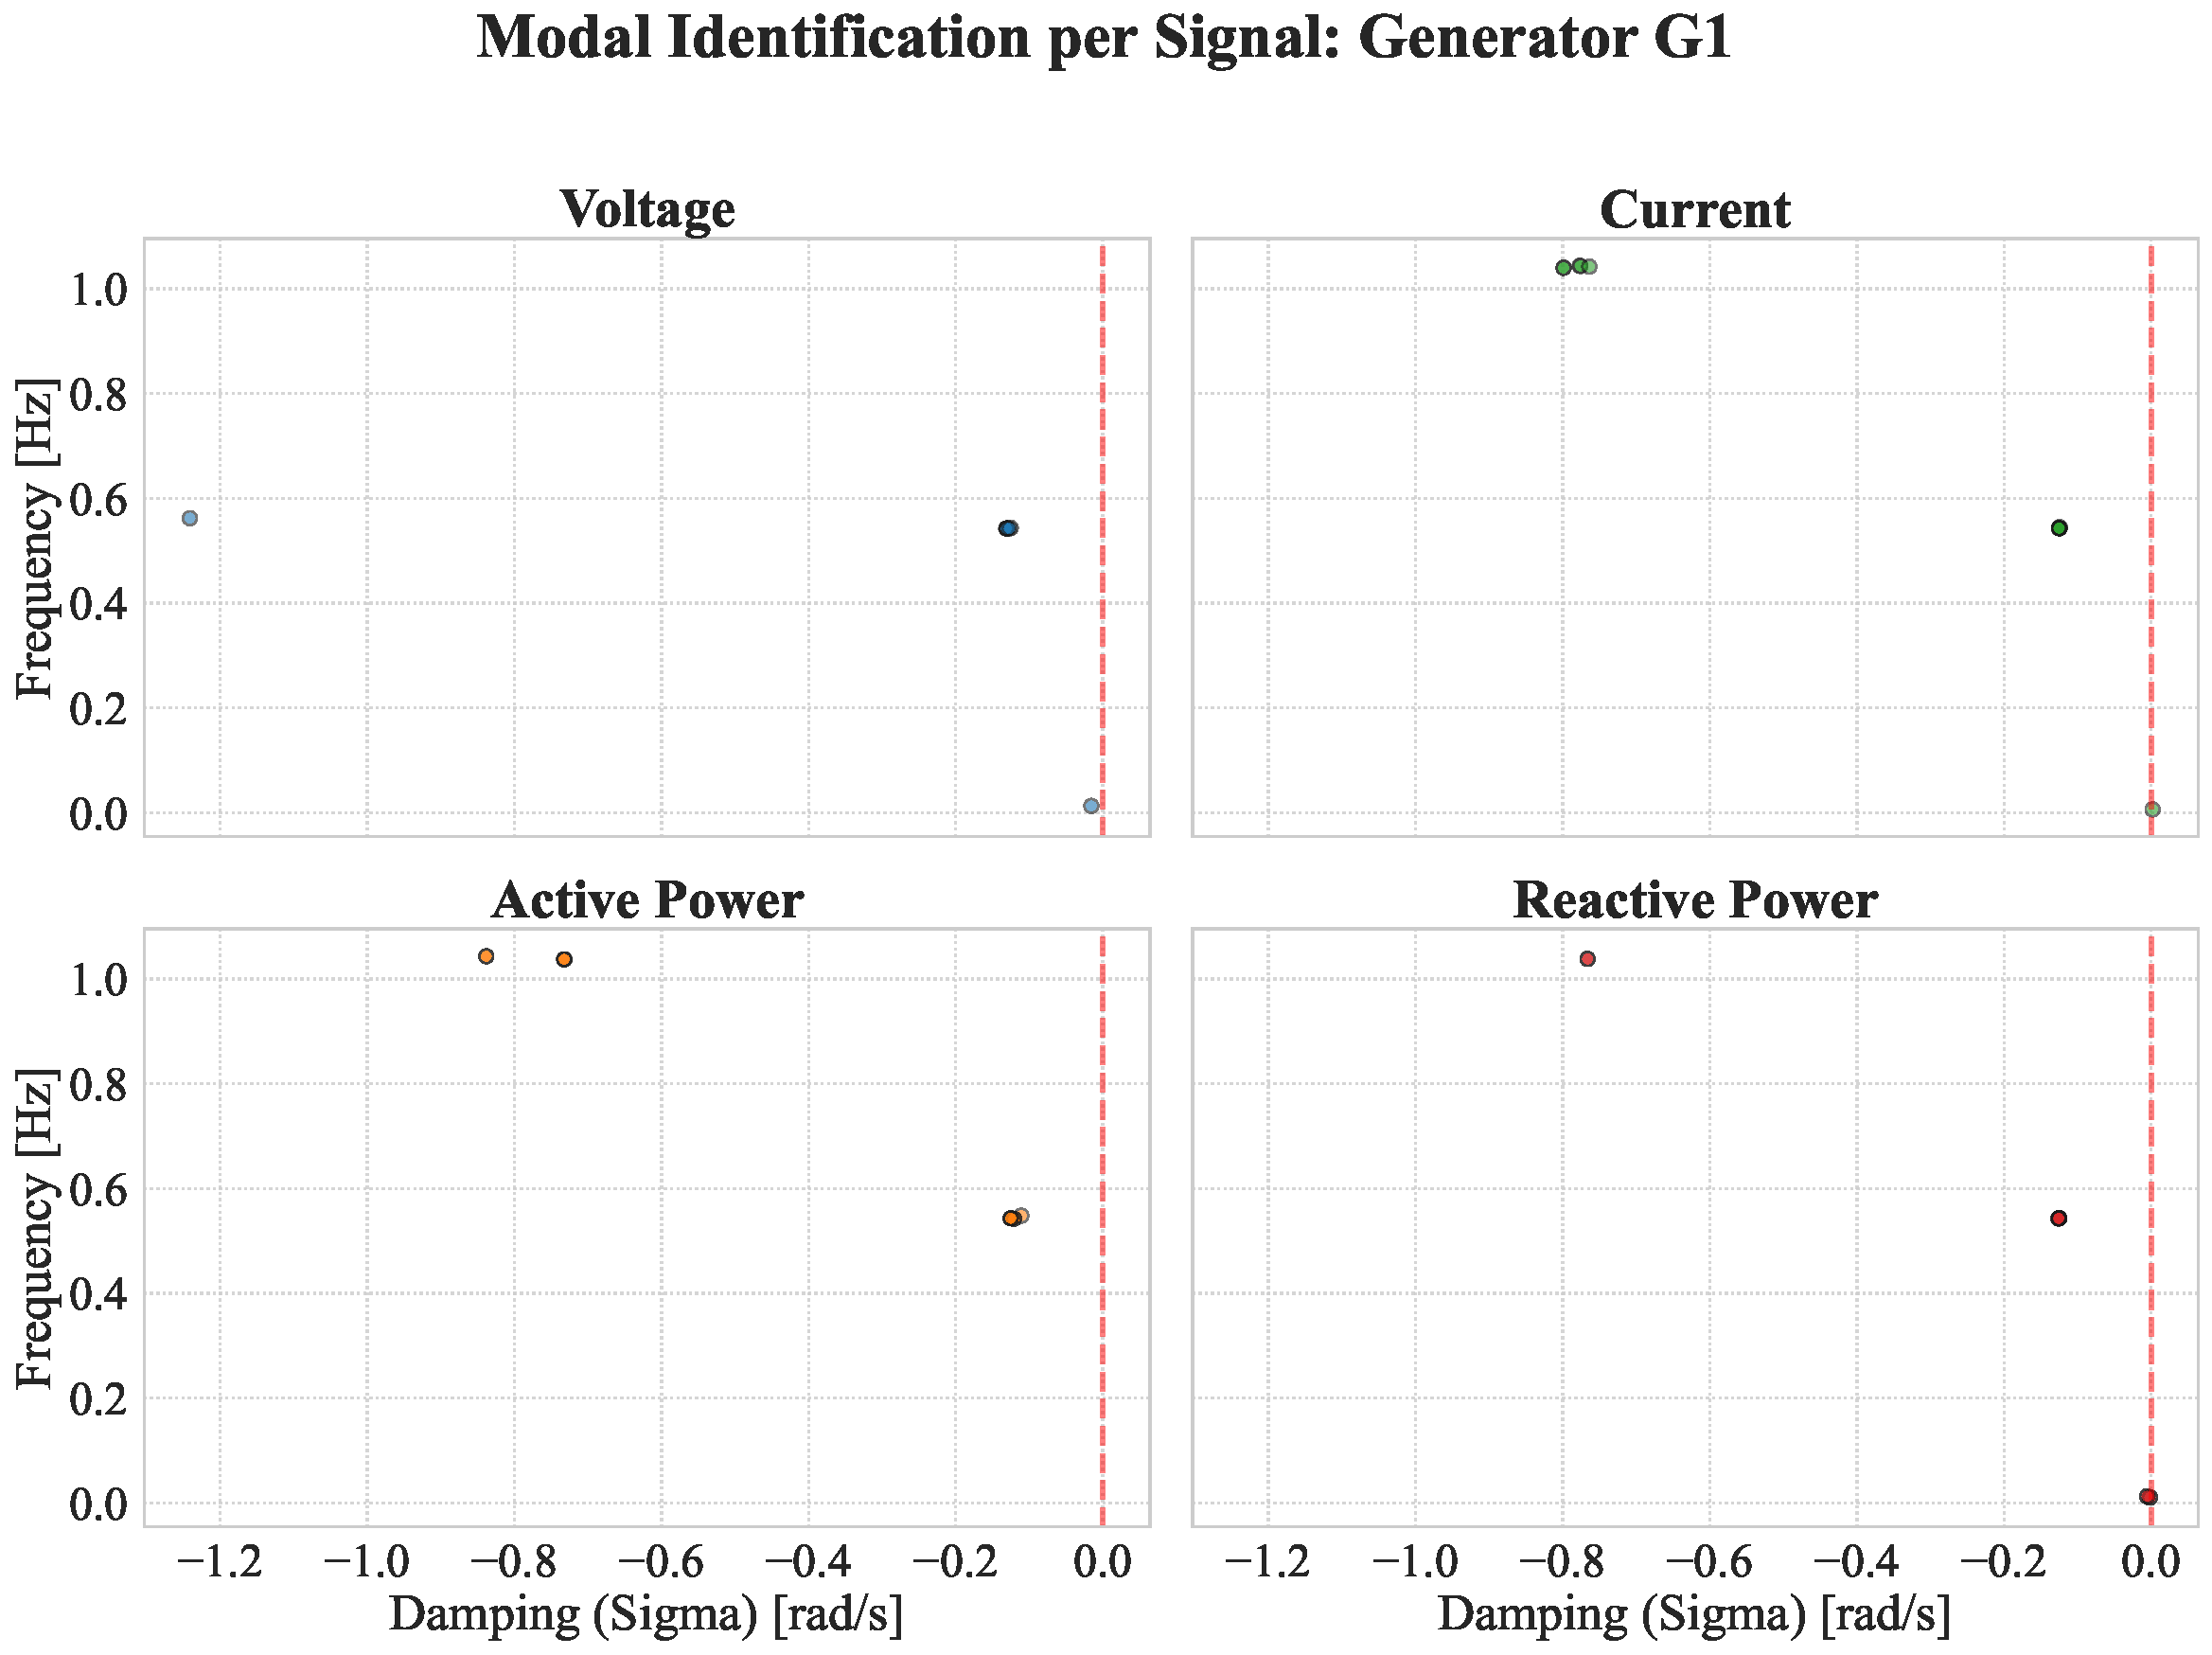
\includegraphics[width=0.95\linewidth]{./plots/modal_maps/pdf/g1_2x2_grid.pdf} 
%     \caption{Κατανομή ιδιοτιμών (\textit{Real Part vs Frequency}) για τη γεννήτρια $G_1$.}
%     \label{fig:poles_distribution_g1}
% \end{figure}

% \begin{figure}[!htbp]
%     \centering
%     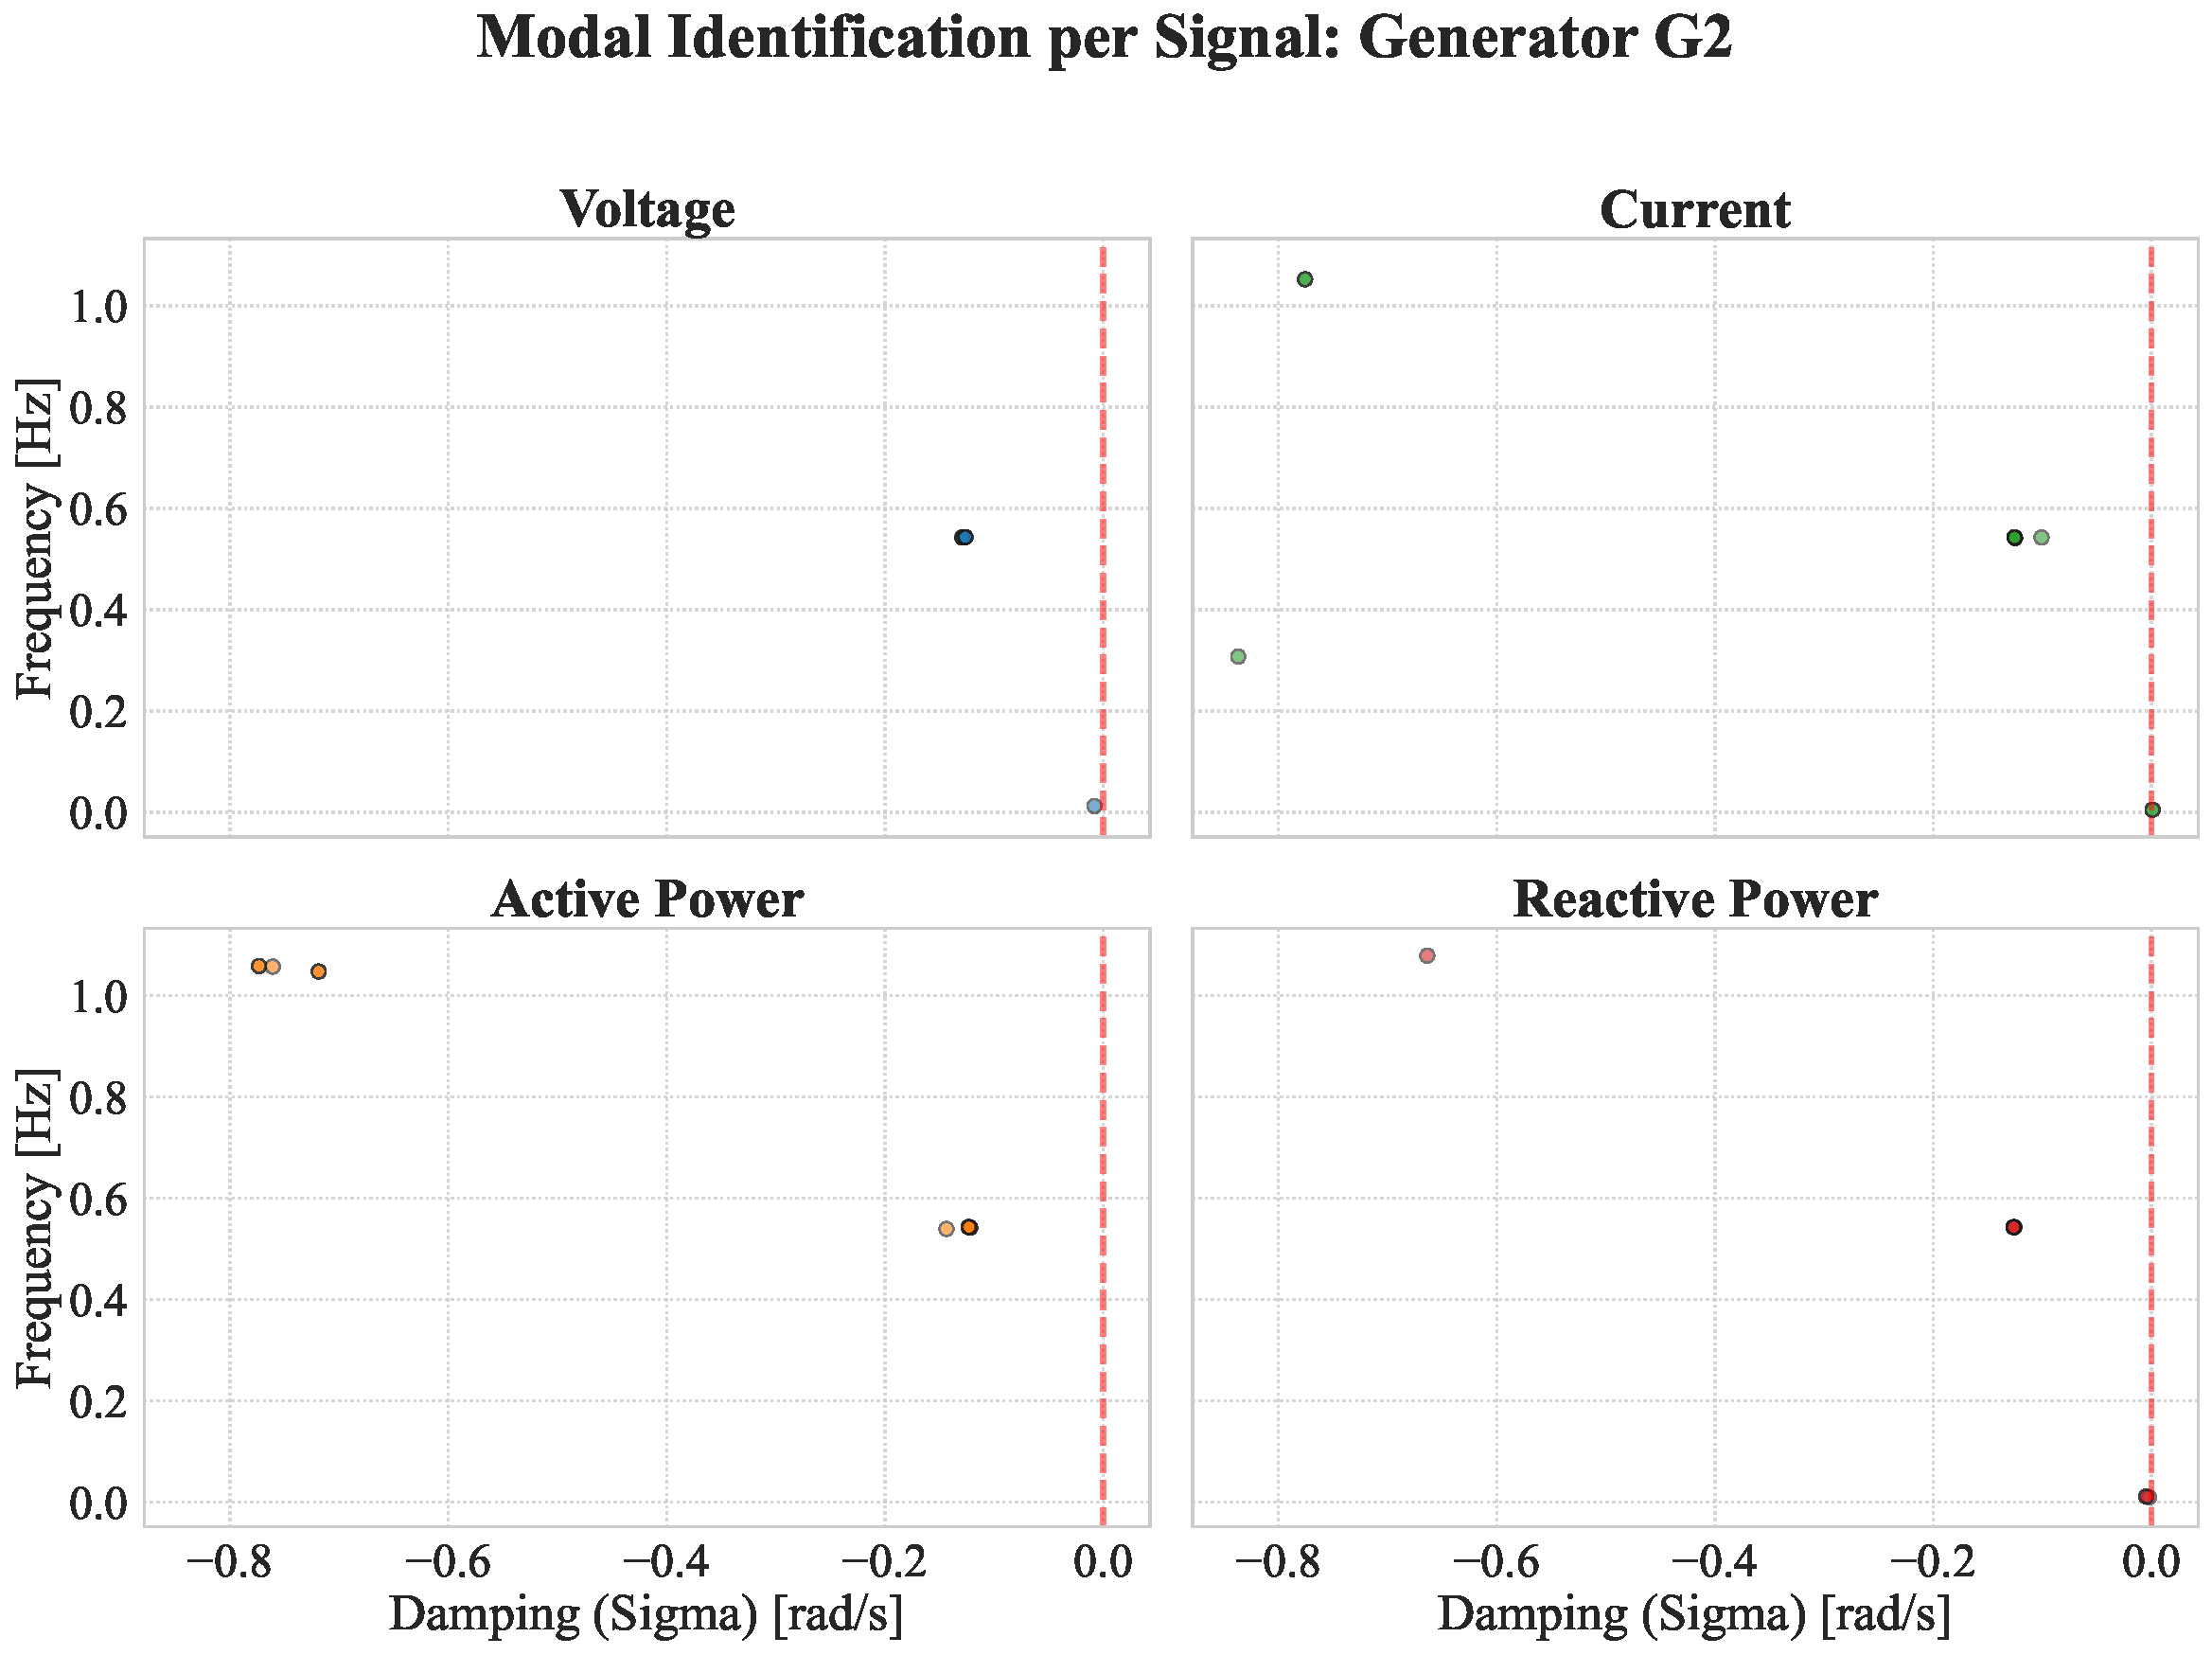
\includegraphics[width=0.95\linewidth]{./plots/modal_maps/pdf/g2_2x2_grid.pdf} 
%     \caption{Κατανομή ιδιοτιμών (\textit{Real Part vs Frequency}) για τη γεννήτρια $G_2$.}
%     \label{fig:poles_distribution_g2}
% \end{figure}

% \begin{figure}[!htbp]
%     \centering
%     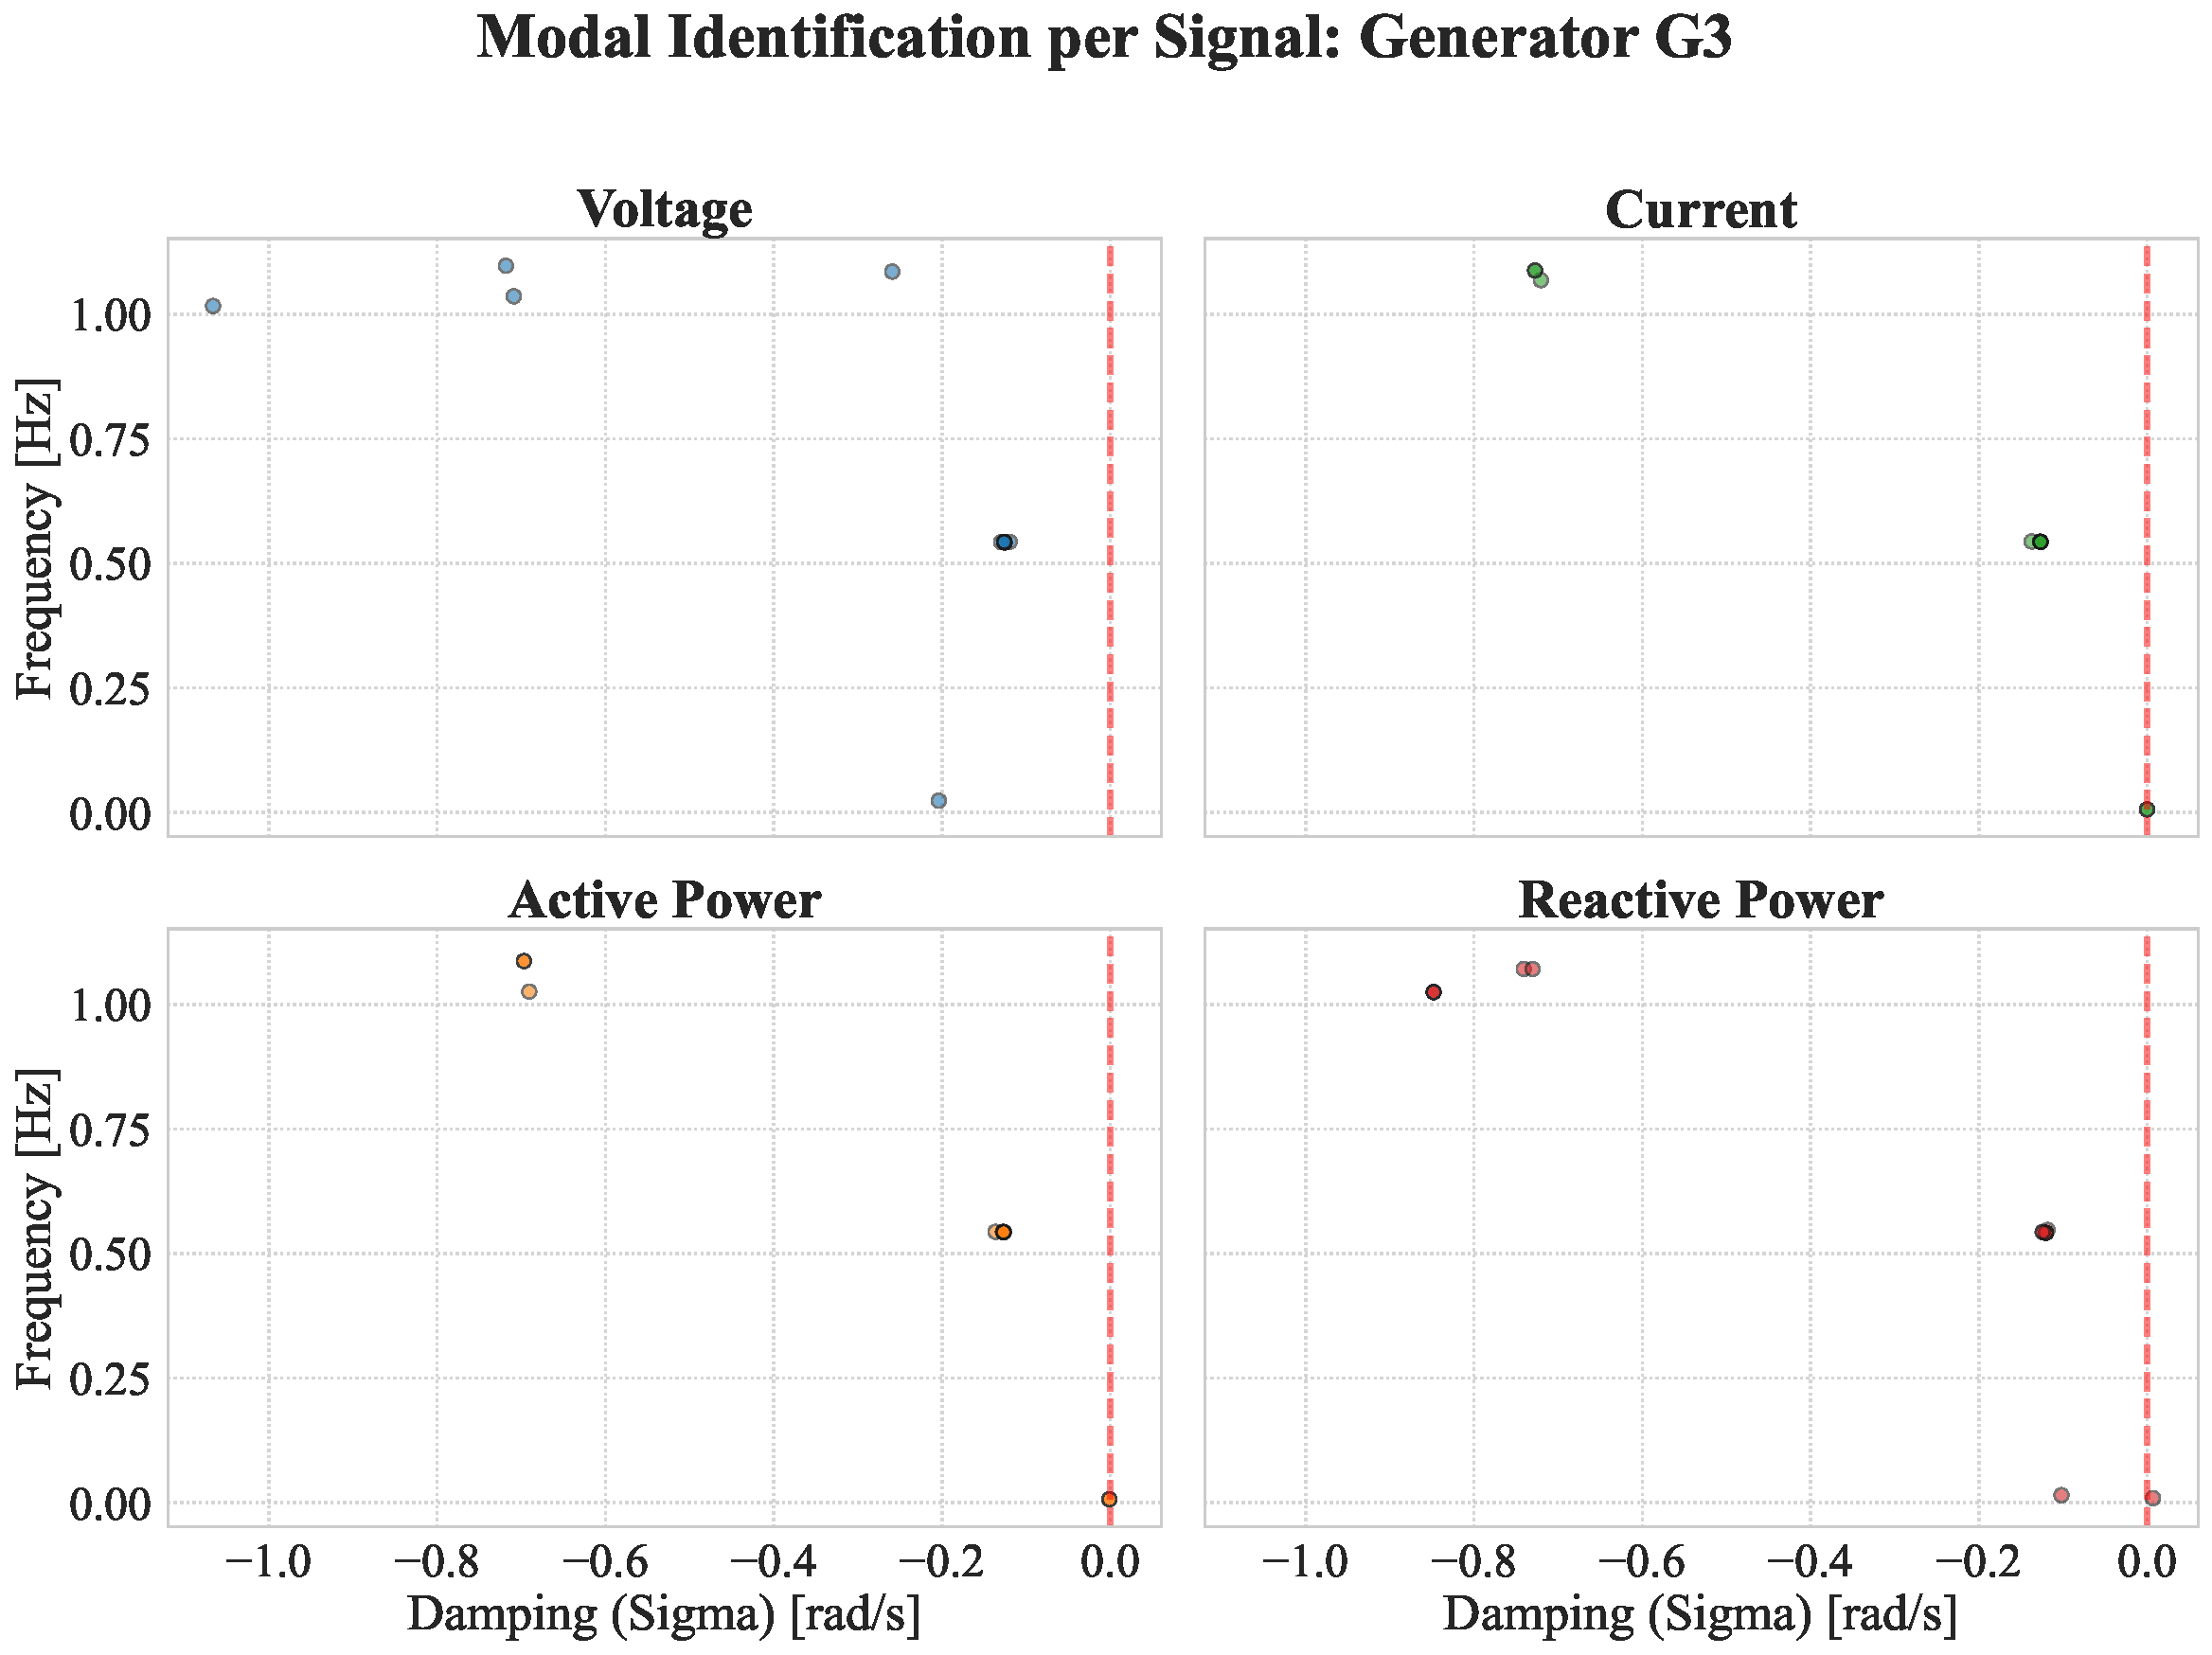
\includegraphics[width=0.95\linewidth]{./plots/modal_maps/pdf/g3_2x2_grid.pdf} 
%     \caption{Κατανομή ιδιοτιμών (\textit{Real Part vs Frequency}) για τη γεννήτρια $G_3$.}
%     \label{fig:poles_distribution_g3}
% \end{figure}

% \begin{figure}[!htbp]
%     \centering
%     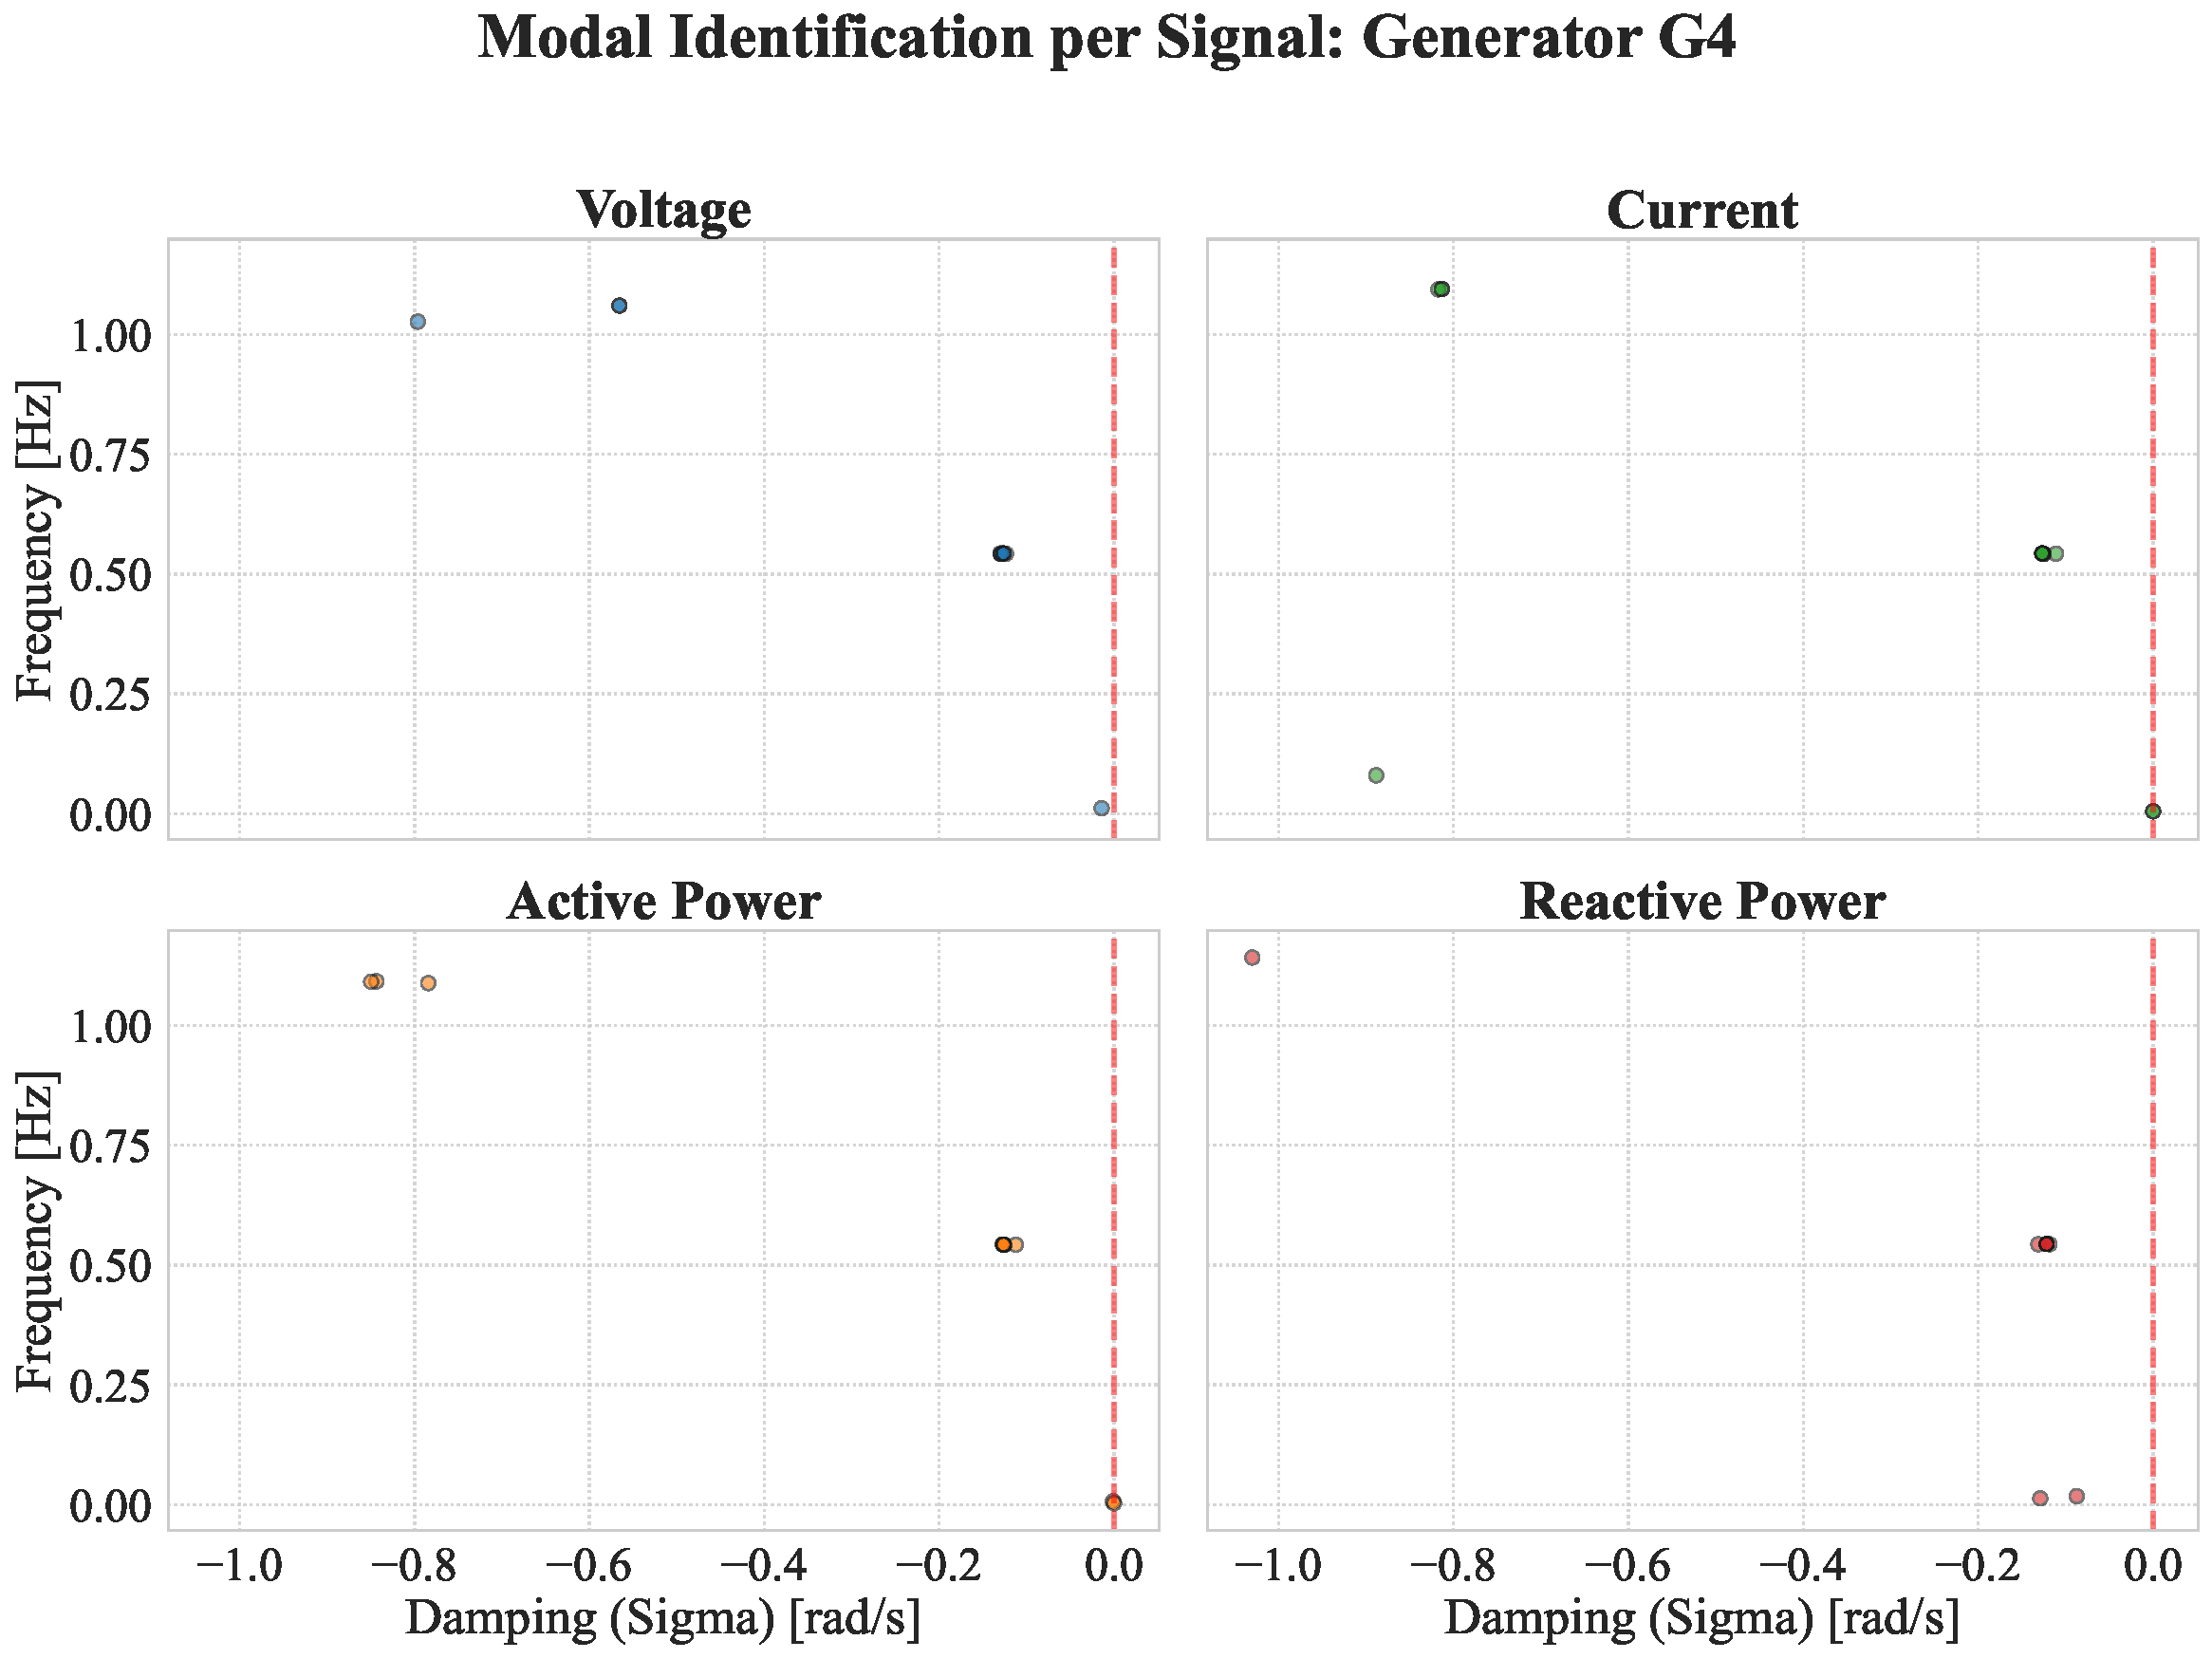
\includegraphics[width=0.95\linewidth]{./plots/modal_maps/pdf/g4_2x2_grid.pdf} 
%     \caption{Κατανομή ιδιοτιμών (\textit{Real Part vs Frequency}) για τη γεννήτρια $G_4$.}
%     \label{fig:poles_distribution_g4}
% \end{figure}

\begin{figure}[!htbp]
    \centering
    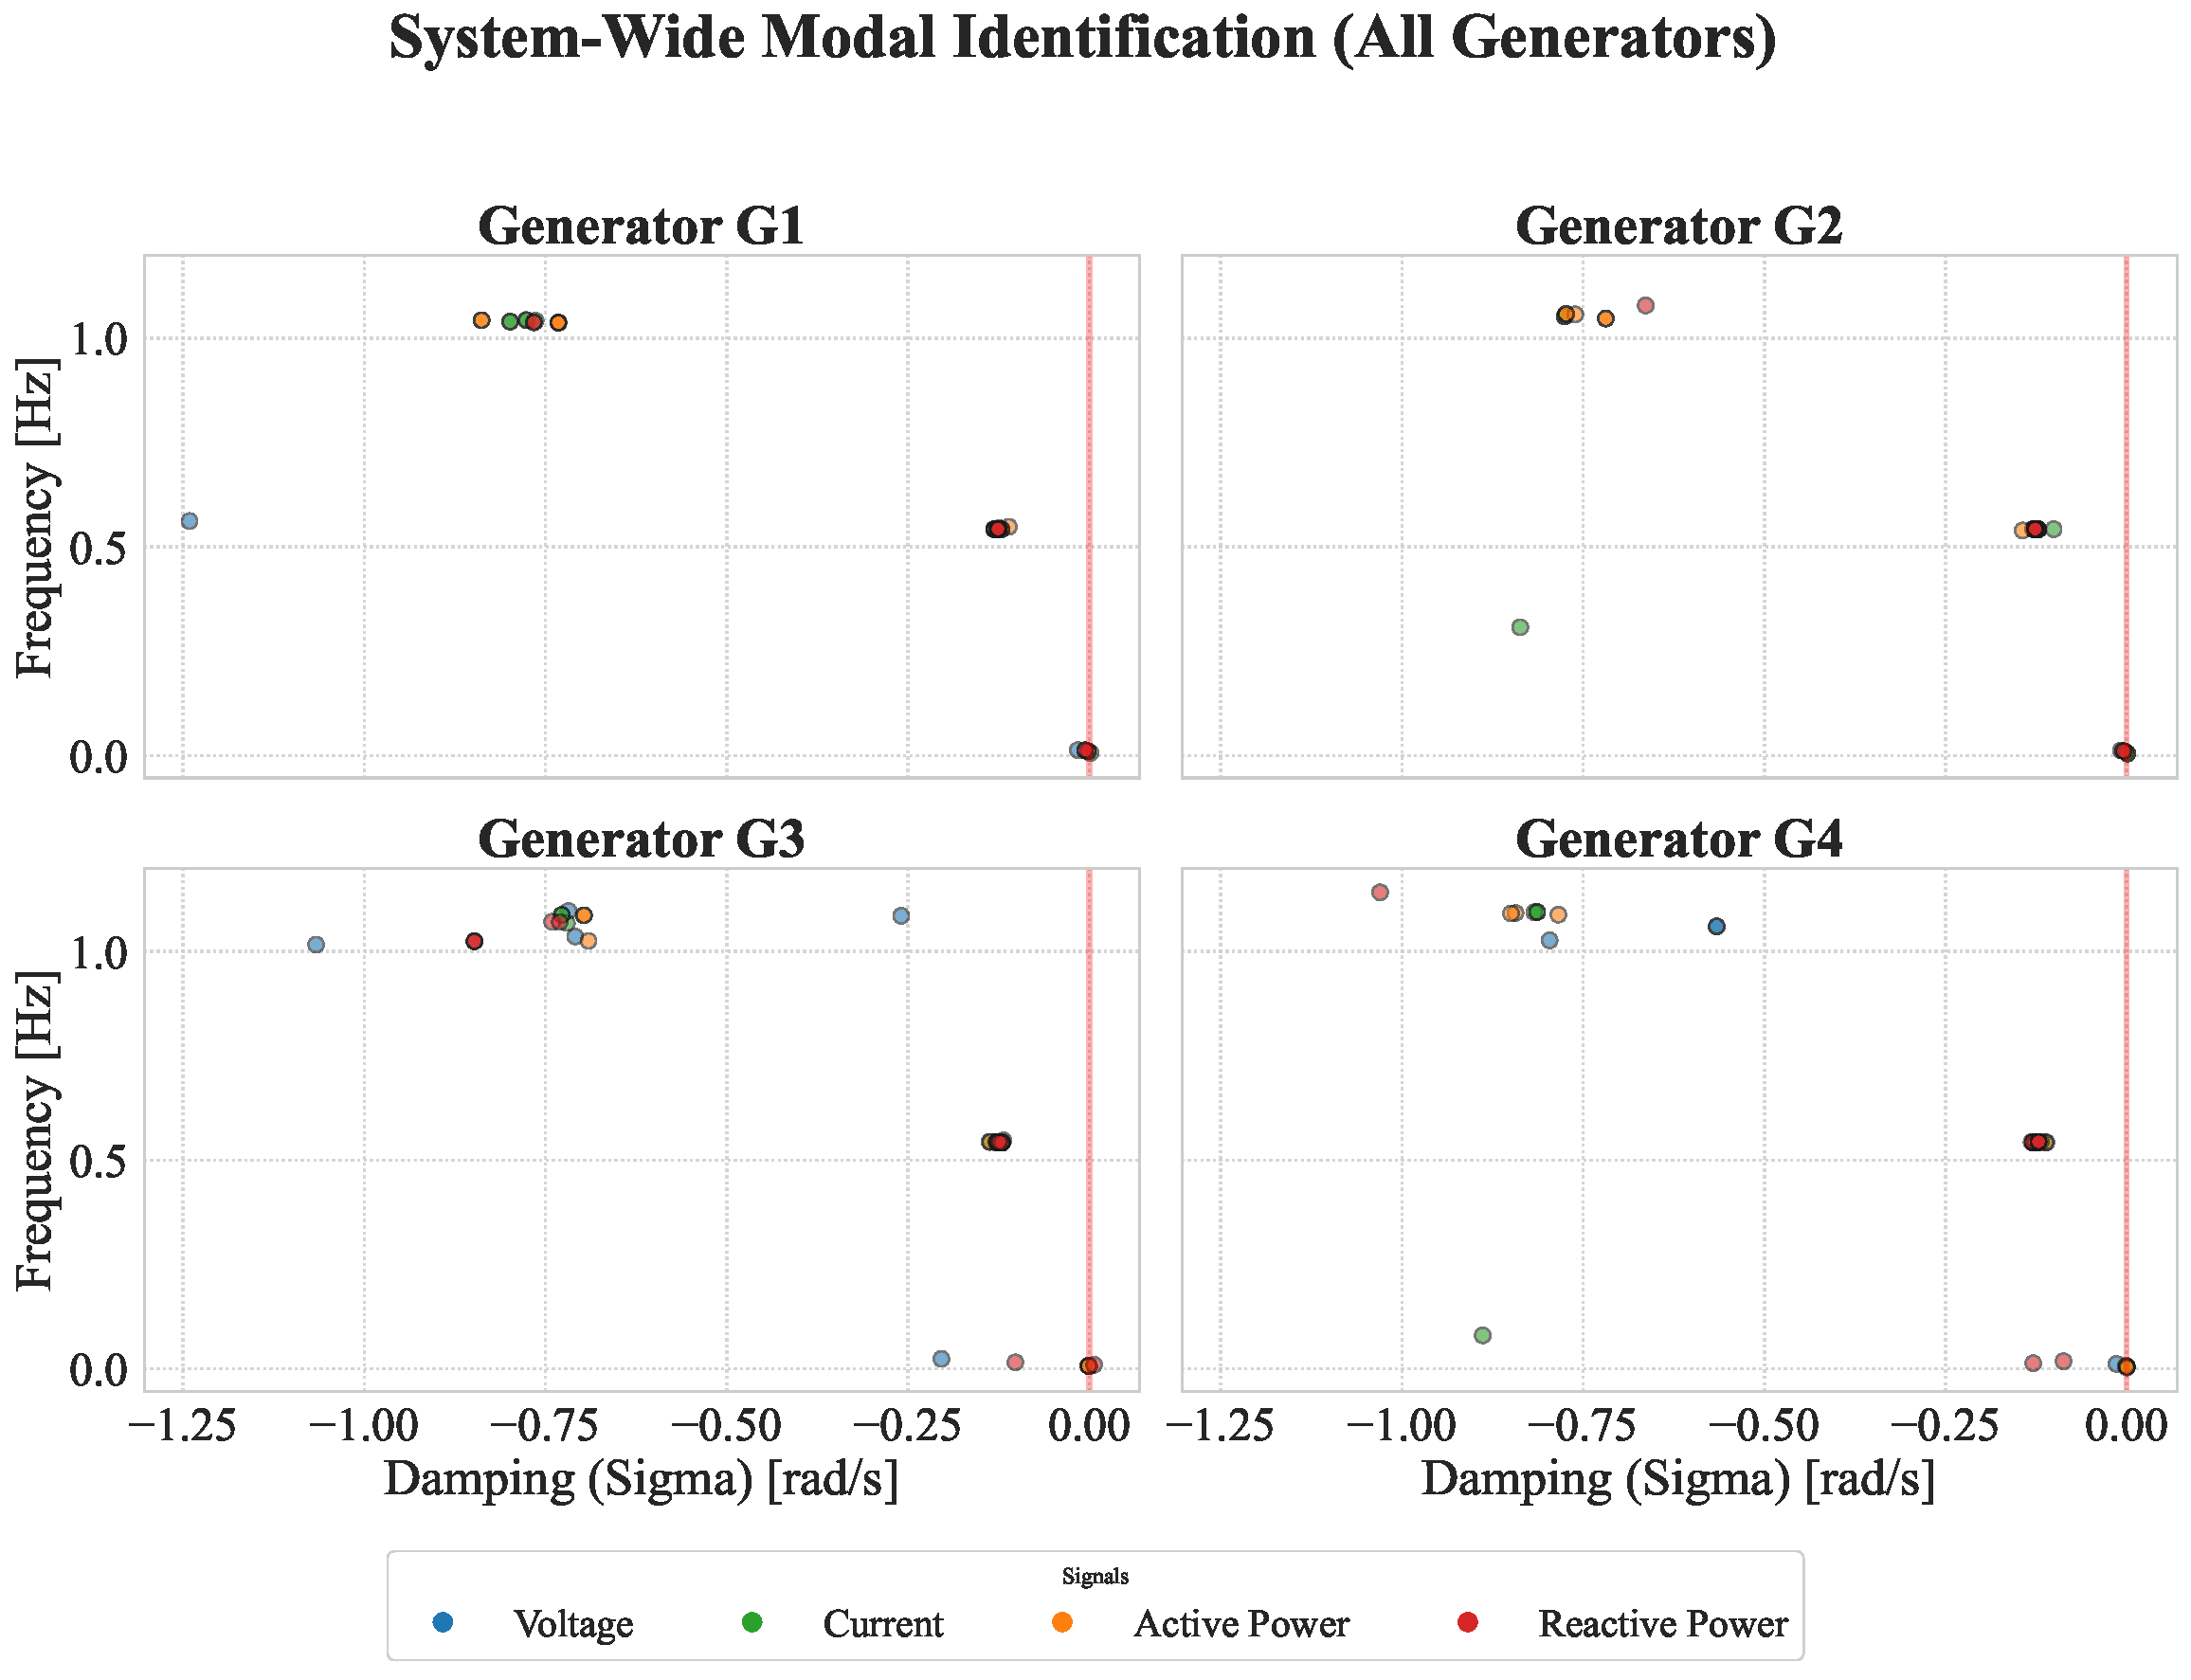
\includegraphics[width=0.95\linewidth]{./plots/modal_maps/pdf/All_Generators_Grid.pdf} 
    \caption{Κατανομή ιδιοτιμών (\textit{Real Part vs Frequency}) για τις γεννήτριες $G_1$-$G_4$ του \textit{Kundur Two-Area System}.}
    \label{fig:poles_distribution_all_kundur}
\end{figure}

% \begin{figure}[!htbp]
%     \centering
%     
\includegraphics[width=0.95\linewidth]{../IEEE39/analysis/Load03_Pplus2_50s_0.2_to_end_reset/plots/modal_maps/pdf/g1_2x2_grid.pdf} 
%     \caption{Κατανομή ιδιοτιμών (\textit{Real Part vs Frequency}) για τη γεννήτρια $G_1$.}
%     \label{fig:poles_distribution_g1_ieee39}
% \end{figure}

\begin{figure}[!htbp]
    \centering
    
\includegraphics[width=0.95\linewidth]{../IEEE39/analysis/Load03_Pplus2_50s_0.2_to_end_reset/plots/modal_maps/pdf/All_Generators_Grid.pdf} 
    \caption{Κατανομή ιδιοτιμών (\textit{Real Part vs Frequency}) για τις γεννήτριες $G_1$-$G_{10}$ του \textit{IEEE 39-Bus System}.}
    \label{fig:poles_distribution_all_ieee39}
\end{figure}


Στο Figure~\ref{fig:poles_distribution_all_kundur} αποτυπώνεται η κατανομή των ταυτοποιημένων ιδιοτιμών για τις τέσσερις γεννήτριες του \textit{Kundur Two-Area System} ($G_1$-$G_4$). Αντίστοιχα, στο Figure~\ref{fig:poles_distribution_all_ieee39} παρουσιάζεται η κατανομή των ιδιοτιμών για τις δέκα γεννήτριες του \textit{IEEE 39-Bus System} ($G_1$-$G_{10}$), συσχετίζοντας τη συχνότητα ταλάντωσης ($f$) με τον ρυθμό απόσβεσης ($\sigma$). Η ανάλυση επιβεβαιώνει την ευστάθεια του συστήματος, καθώς σχεδόν το σύνολο των σημείων εντοπίζεται στο αριστερό ημιεπίπεδο (αρνητικό $\sigma$), υποδεικνύοντας τη θετική απόσβεση των ταλαντώσεων. 
% Ιδιαίτερα σημαντική είναι η έντονη ομαδοποίηση σημείων στην περιοχή των $0.5$-$0.6$ Hz, η οποία εμφανίζεται ομοιόμορφα σε όλες τις γεννήτριες και σε όλα τα καταγεγραμμένα σήματα ($V$, $I$, $P$, $Q$), αποτελώντας ένδειξη του κύριου τρόπου ταλάντωσης (\textit{inter-area}) του συστήματος \textit{Kundur Two-Area System}. Επιπρόσθετα, διακρίνονται διακριτές συστάδες στην περιοχή του $1.0$ έως $1.2$ Hz, οι οποίες αντιστοιχούν στις τοπικές ταλαντώσεις (\textit{intra-area}) των μηχανών εντός της εκάστοτε περιοχής.
 Ακόμα, καταγράφονται στον οριζόντιο άξονα και ιδιοτιμές με μηδενική συχνότητα, οι οποίες δεν αντιστοιχούν σε κύριους ταλαντωτικούς ρυθμούς, αλλά σε μη ταλαντωτικές ή πολύ αργές συνιστώσες της απόκρισης, καθώς και σε αριθμητικά artifacts της μεθόδου.

\subsection{Αξιολόγηση Πιστότητας Ανακατασκευής (\textit{Signal Reconstruction})}
Για την επαλήθευση της εγκυρότητας των ιδιοτιμών που εξήχθησαν στην προηγούμενη ενότητα, πραγματοποιήθηκε μαθηματική ανακατασκευή των σημάτων στο πεδίο του χρόνου. Αρχικά, εξετάστηκε η συμπεριφορά των επιμέρους προσεγγίσεων (σταθερής τάξης $n$ και ανοχής $\tau$) προκειμένου να αξιολογηθεί η επίδραση τους στην ακρίβεια της προσαρμογής όπως φαίνεται στα Figures~\ref{fig:g1_reactive_power_reconstruction_kundur} και \ref{fig:g1_reactive_power_reconstruction_ieee39}.

\begin{figure}[htbp]
    \centering
    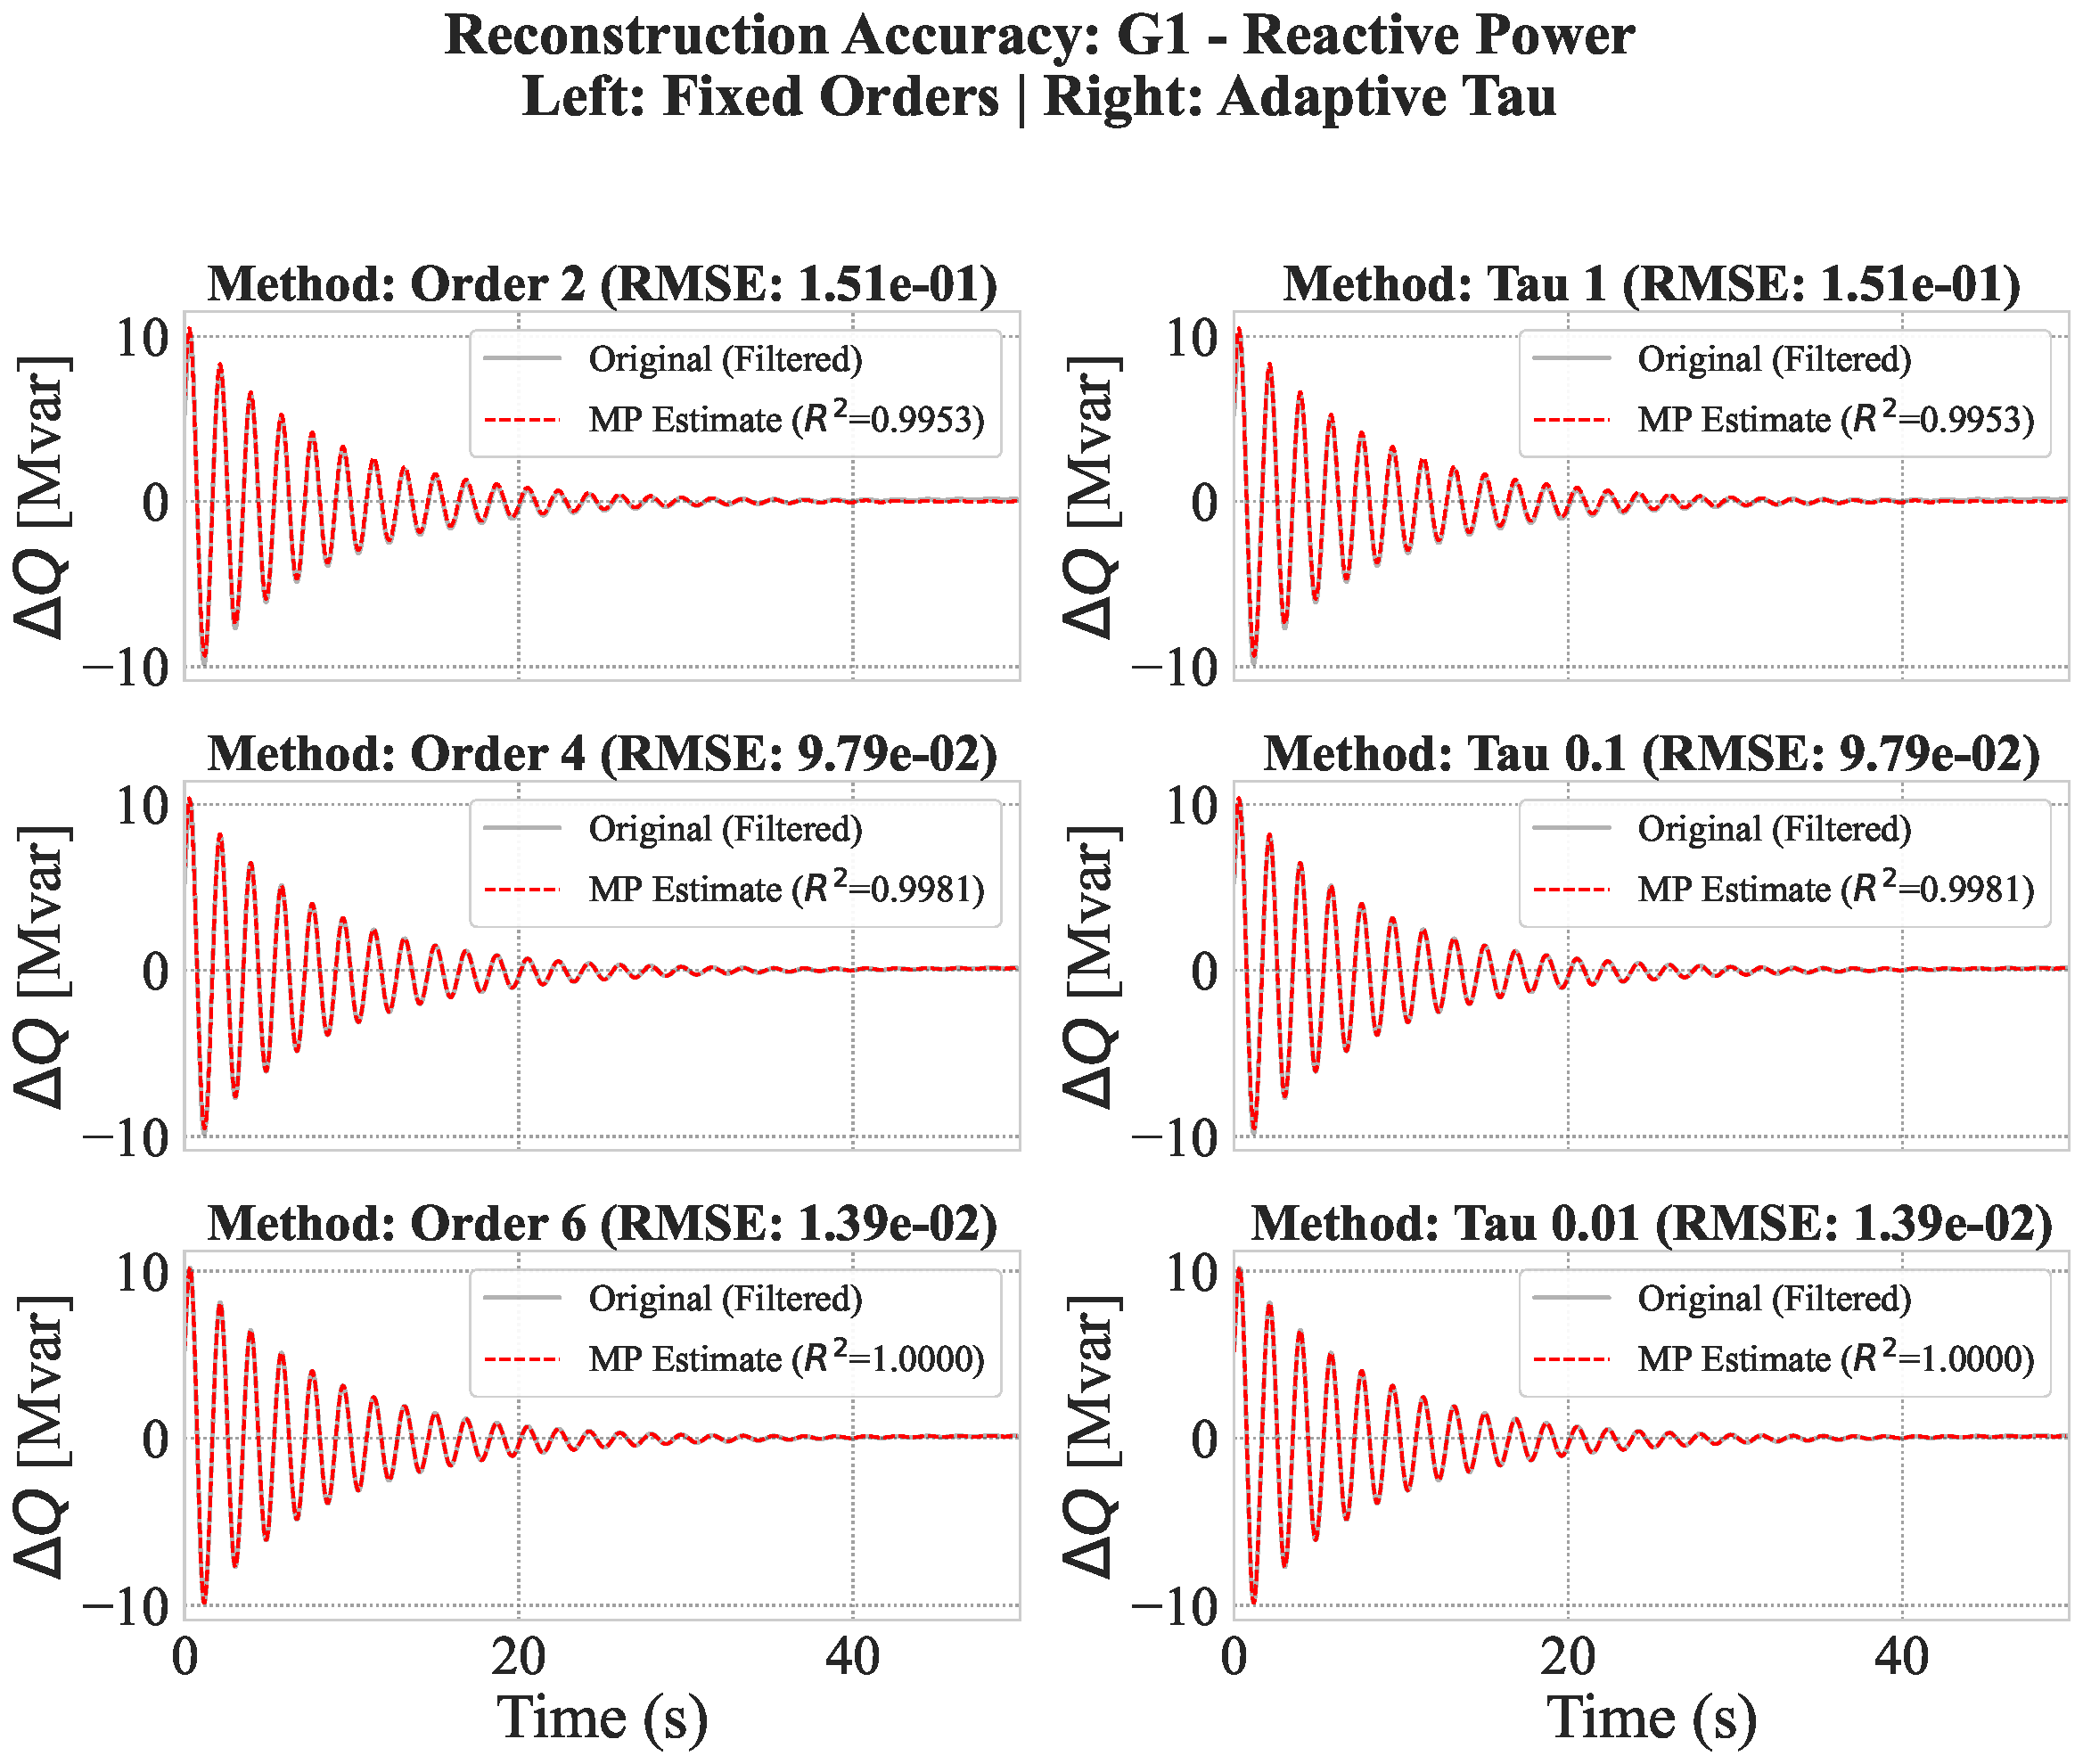
\includegraphics[width=0.95\linewidth]{./plots/reconstruction_grids/pdf/g1_Reactive_Power_Reconstruction.pdf} 
    \caption{Ανακατασκευή σήματος αέργου ισχύος ($Q$) για τη γεννήτρια $G_1$ του \textit{Kundur Two-Area System}.}
    \label{fig:g1_reactive_power_reconstruction_kundur}
\end{figure}

\begin{figure}[htbp]
    \centering
    \includegraphics[width=0.95\linewidth]{../IEEE39/analysis/Load03_Pplus2_50s_0.2_to_end_reset/plots/reconstruction_grids/pdf/g1_Reactive_Power_reconstruction.pdf} 
    \caption{Ανακατασκευή σήματος αέργου ισχύος ($Q$) για τη γεννήτρια $G_1$ του \textit{IEEE 39-Bus System}.}
    \label{fig:g1_reactive_power_reconstruction_ieee39}
\end{figure}

Στη συνέχεια, δημιουργήθηκαν επιμέρους διαγράμματα για κάθε γεννήτρια του \textit{Kundur Two-Area System} (Figures \ref{fig:best_recon_g1_kundur} έως \ref{fig:best_recon_g4_kundur}) και γιά ορισμένες γεννήτριες του \textit{IEEE 39-Bus System} (Figures \ref{fig:best_recon_g9_ieee39} έως \ref{fig:best_recon_g6_ieee39}) οι οποίες ανήκουν σε τρεις διακριτές περιοχές ελέγχου ~\cite{sfetkos2024measurement}, τα οποία αποτυπώνουν την άμεση σύγκριση μεταξύ των αρχικών σημάτων (\textit{Original Filtered}) και των αντίστοιχων εκτιμώμενων κυματομορφών (\textit{MP estimate}). Για την τελική ανακατασκευή επιλέχθηκε αυστηρά η μέθοδος που απέδωσε την υψηλότερη ακρίβεια (Max $R^2$) για το εκάστοτε σήμα.

\begin{figure}[htbp]
    \centering
    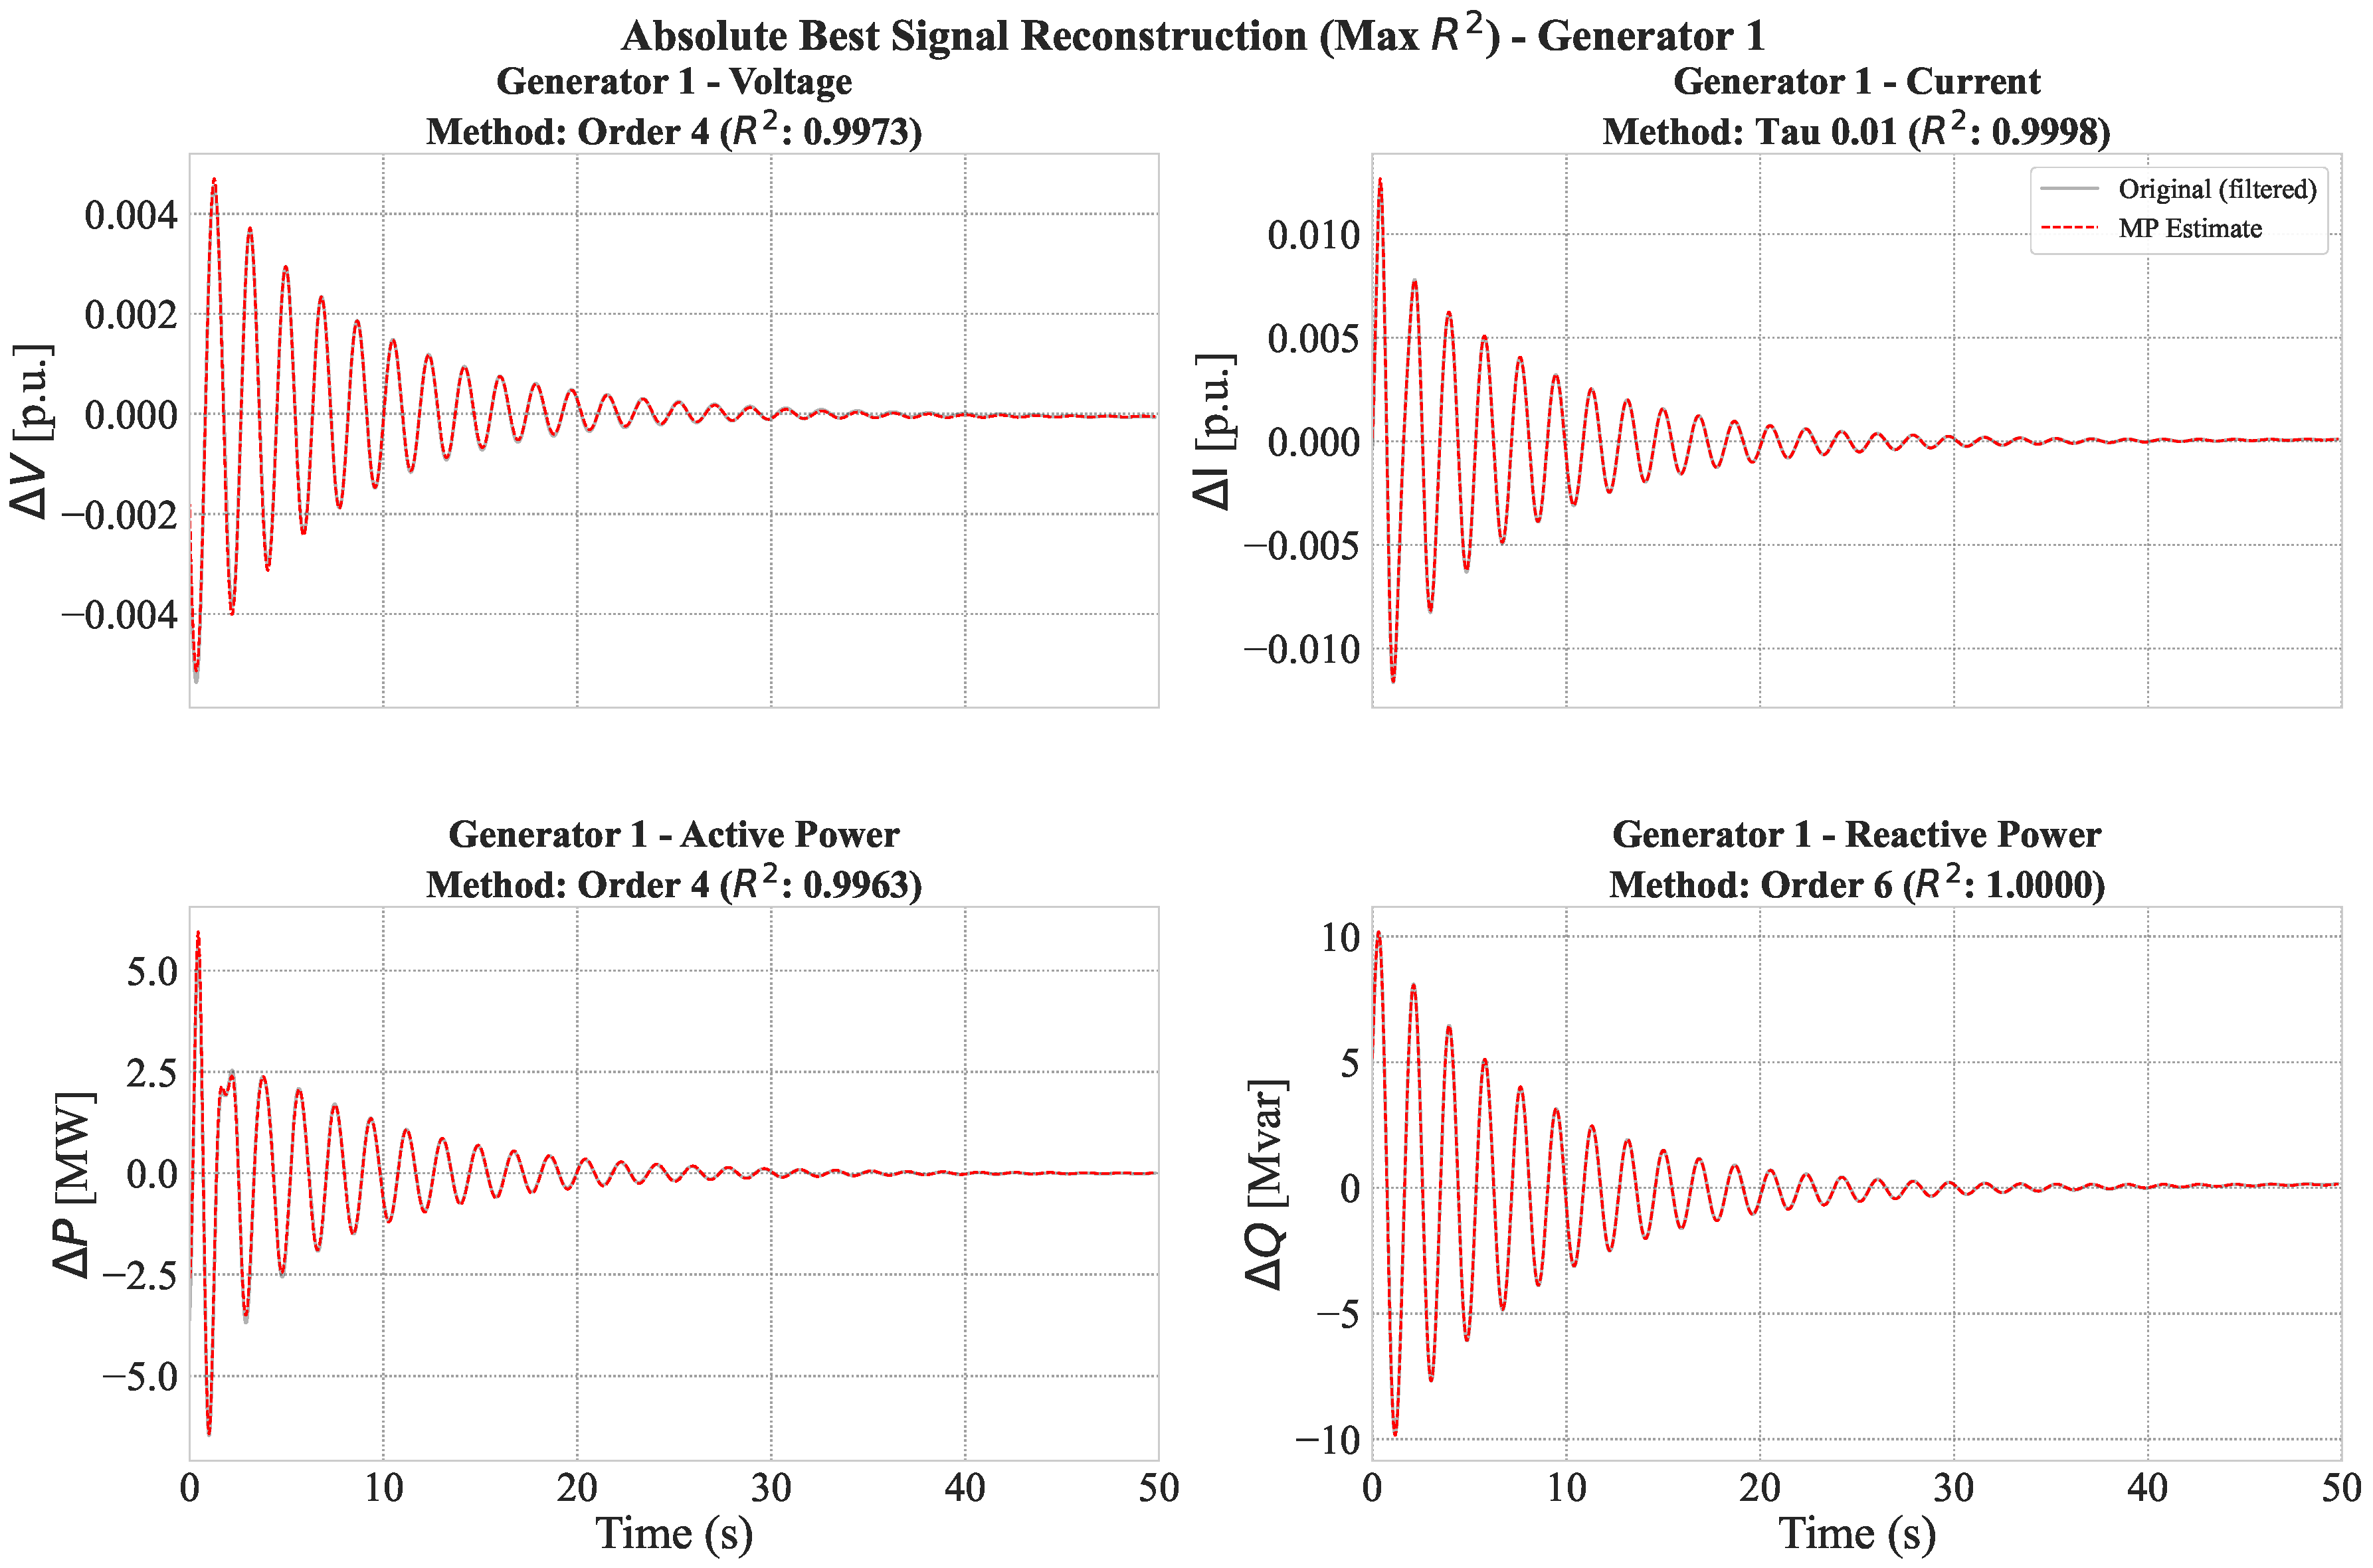
\includegraphics[width=0.95\linewidth]{./stats/pdf/10_best_reconstruction_g1_2x2.pdf} 
    \caption{Βέλτιστη μαθηματική ανακατασκευή των σημάτων ($V, I, P, Q$) για τη γεννήτρια $G_1$ του \textit{Kundur Two-Area System} με βάση τον μέγιστο συντελεστή προσδιορισμού $R^2$.}
    \label{fig:best_recon_g1_kundur}
\end{figure}

\begin{figure}[htbp]
    \centering
    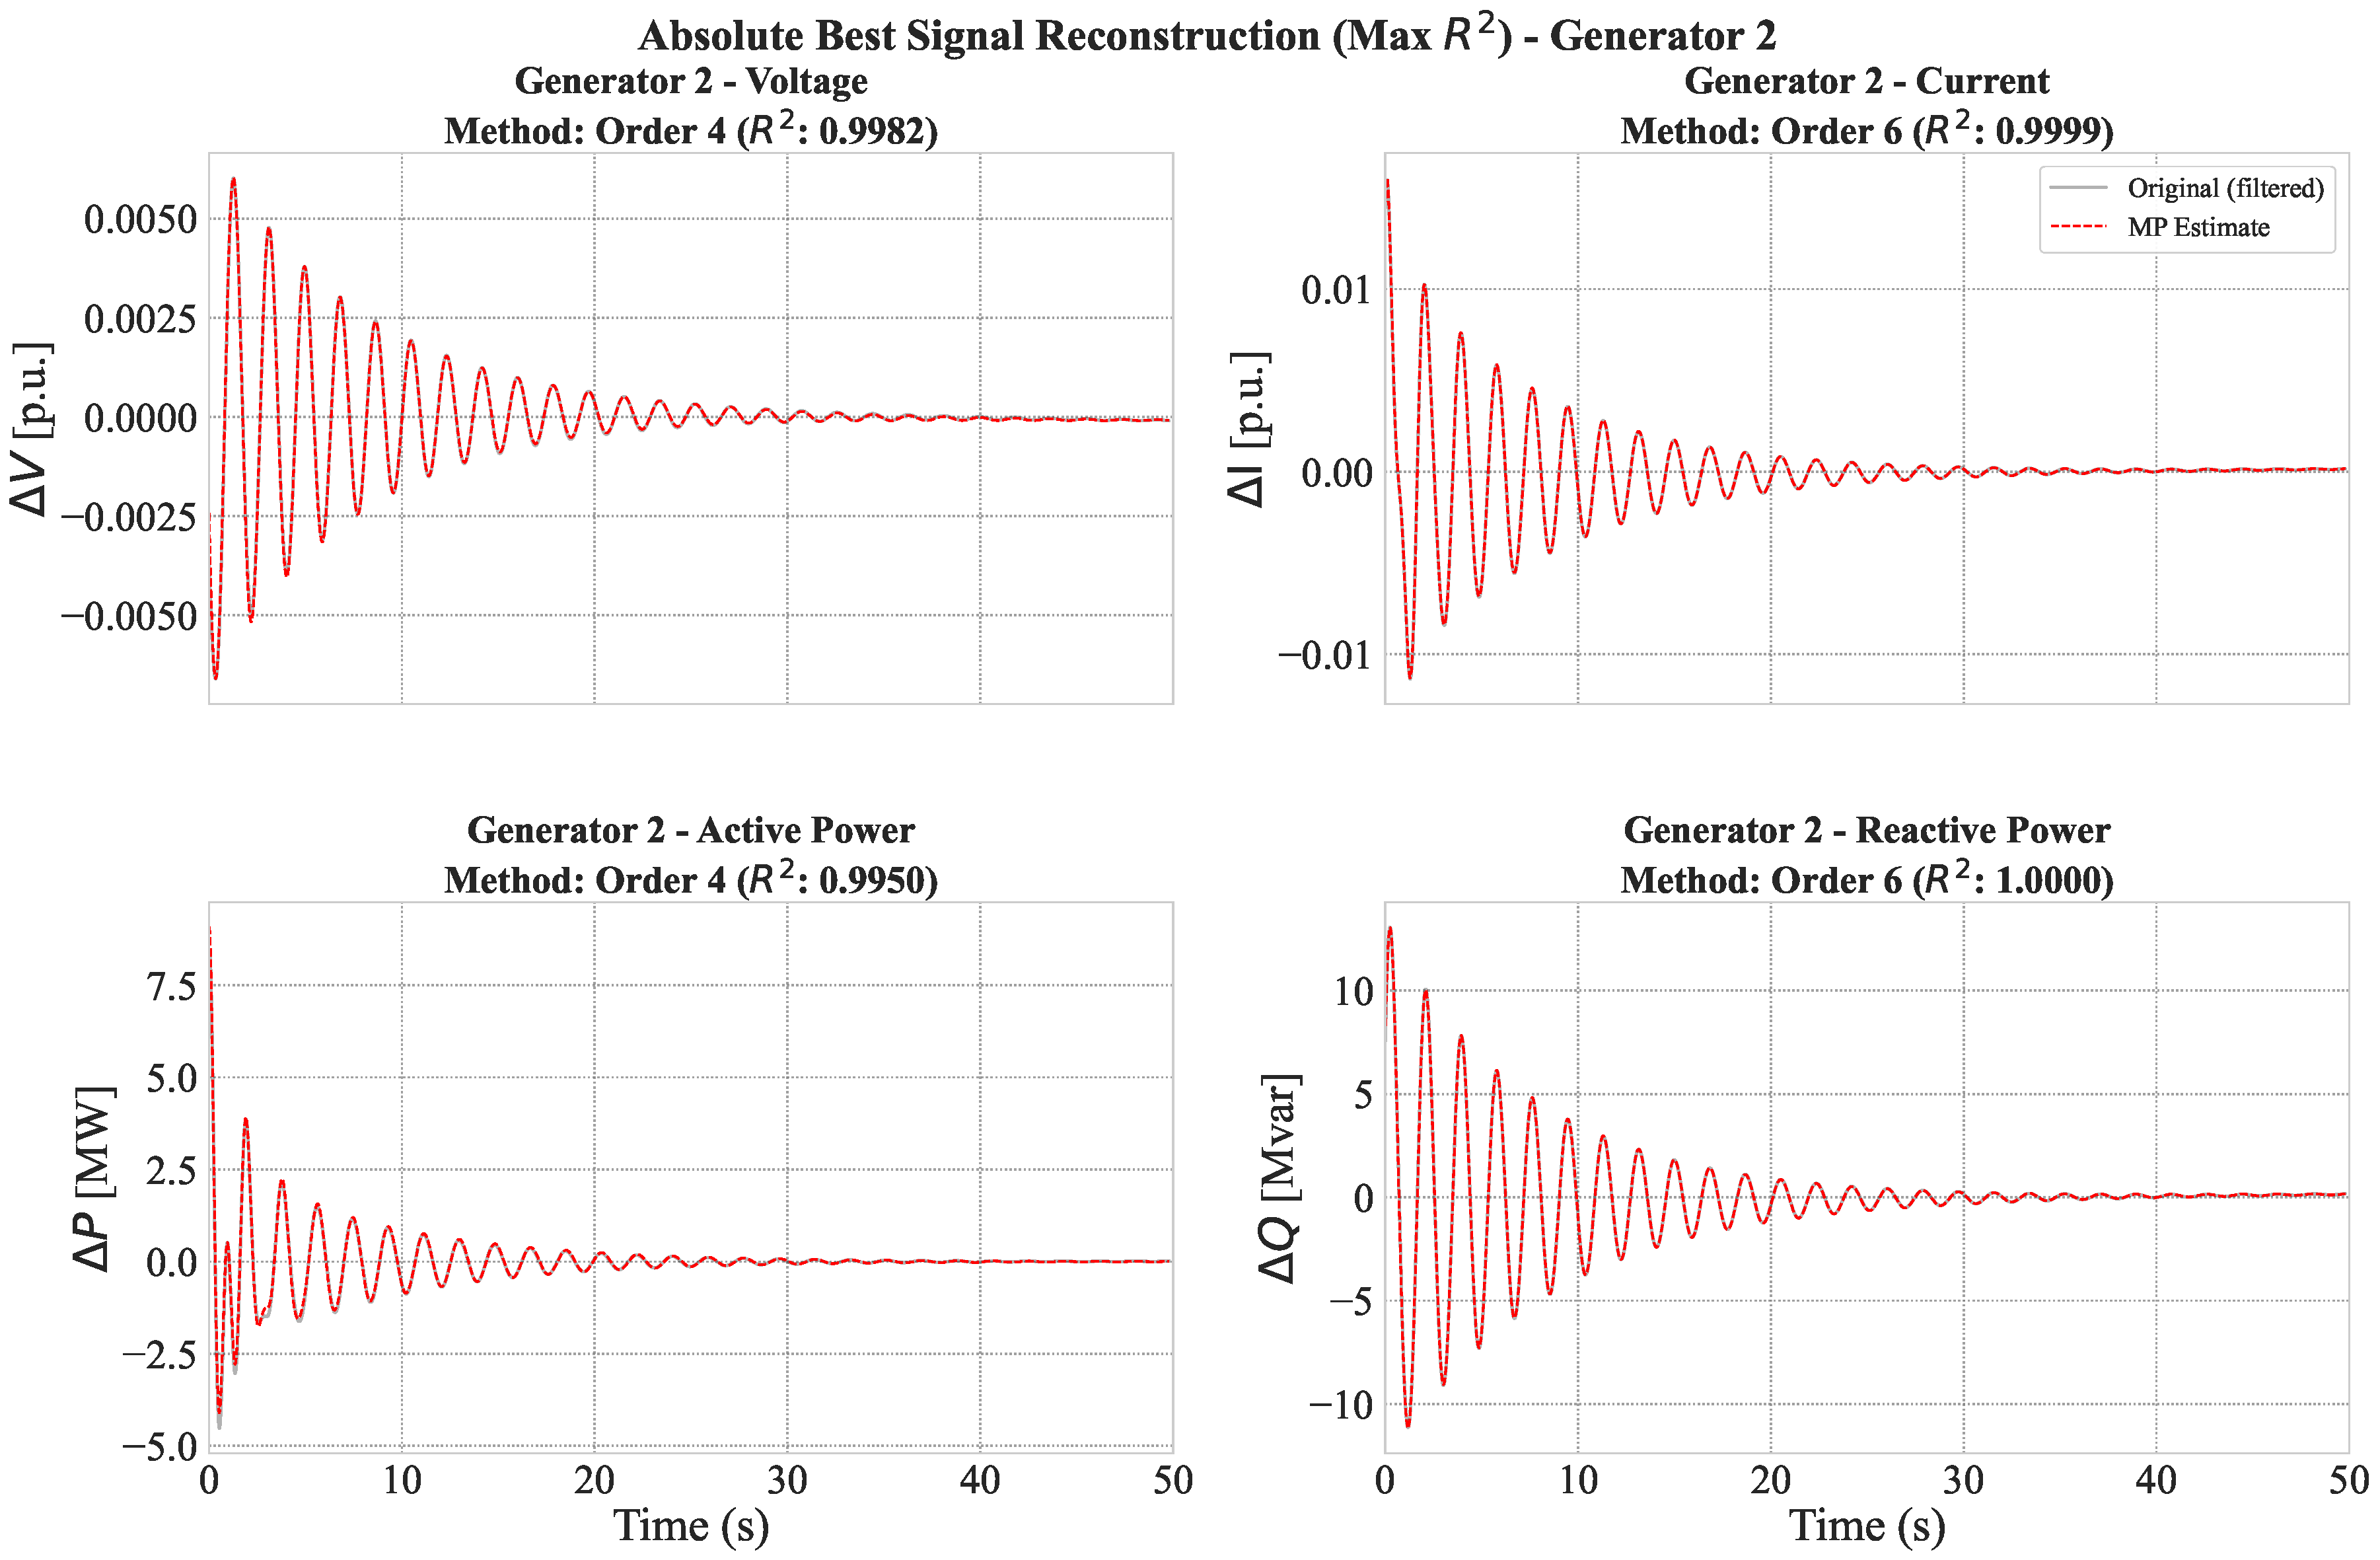
\includegraphics[width=0.95\linewidth]{./stats/pdf/10_best_reconstruction_g2_2x2.pdf} 
    \caption{Βέλτιστη μαθηματική ανακατασκευή των σημάτων ($V, I, P, Q$) για τη γεννήτρια $G_2$ του \textit{Kundur Two-Area System} με βάση τον μέγιστο συντελεστή προσδιορισμού $R^2$.}
    \label{fig:best_recon_g2_kundur}
\end{figure}

\begin{figure}[htbp]
    \centering
    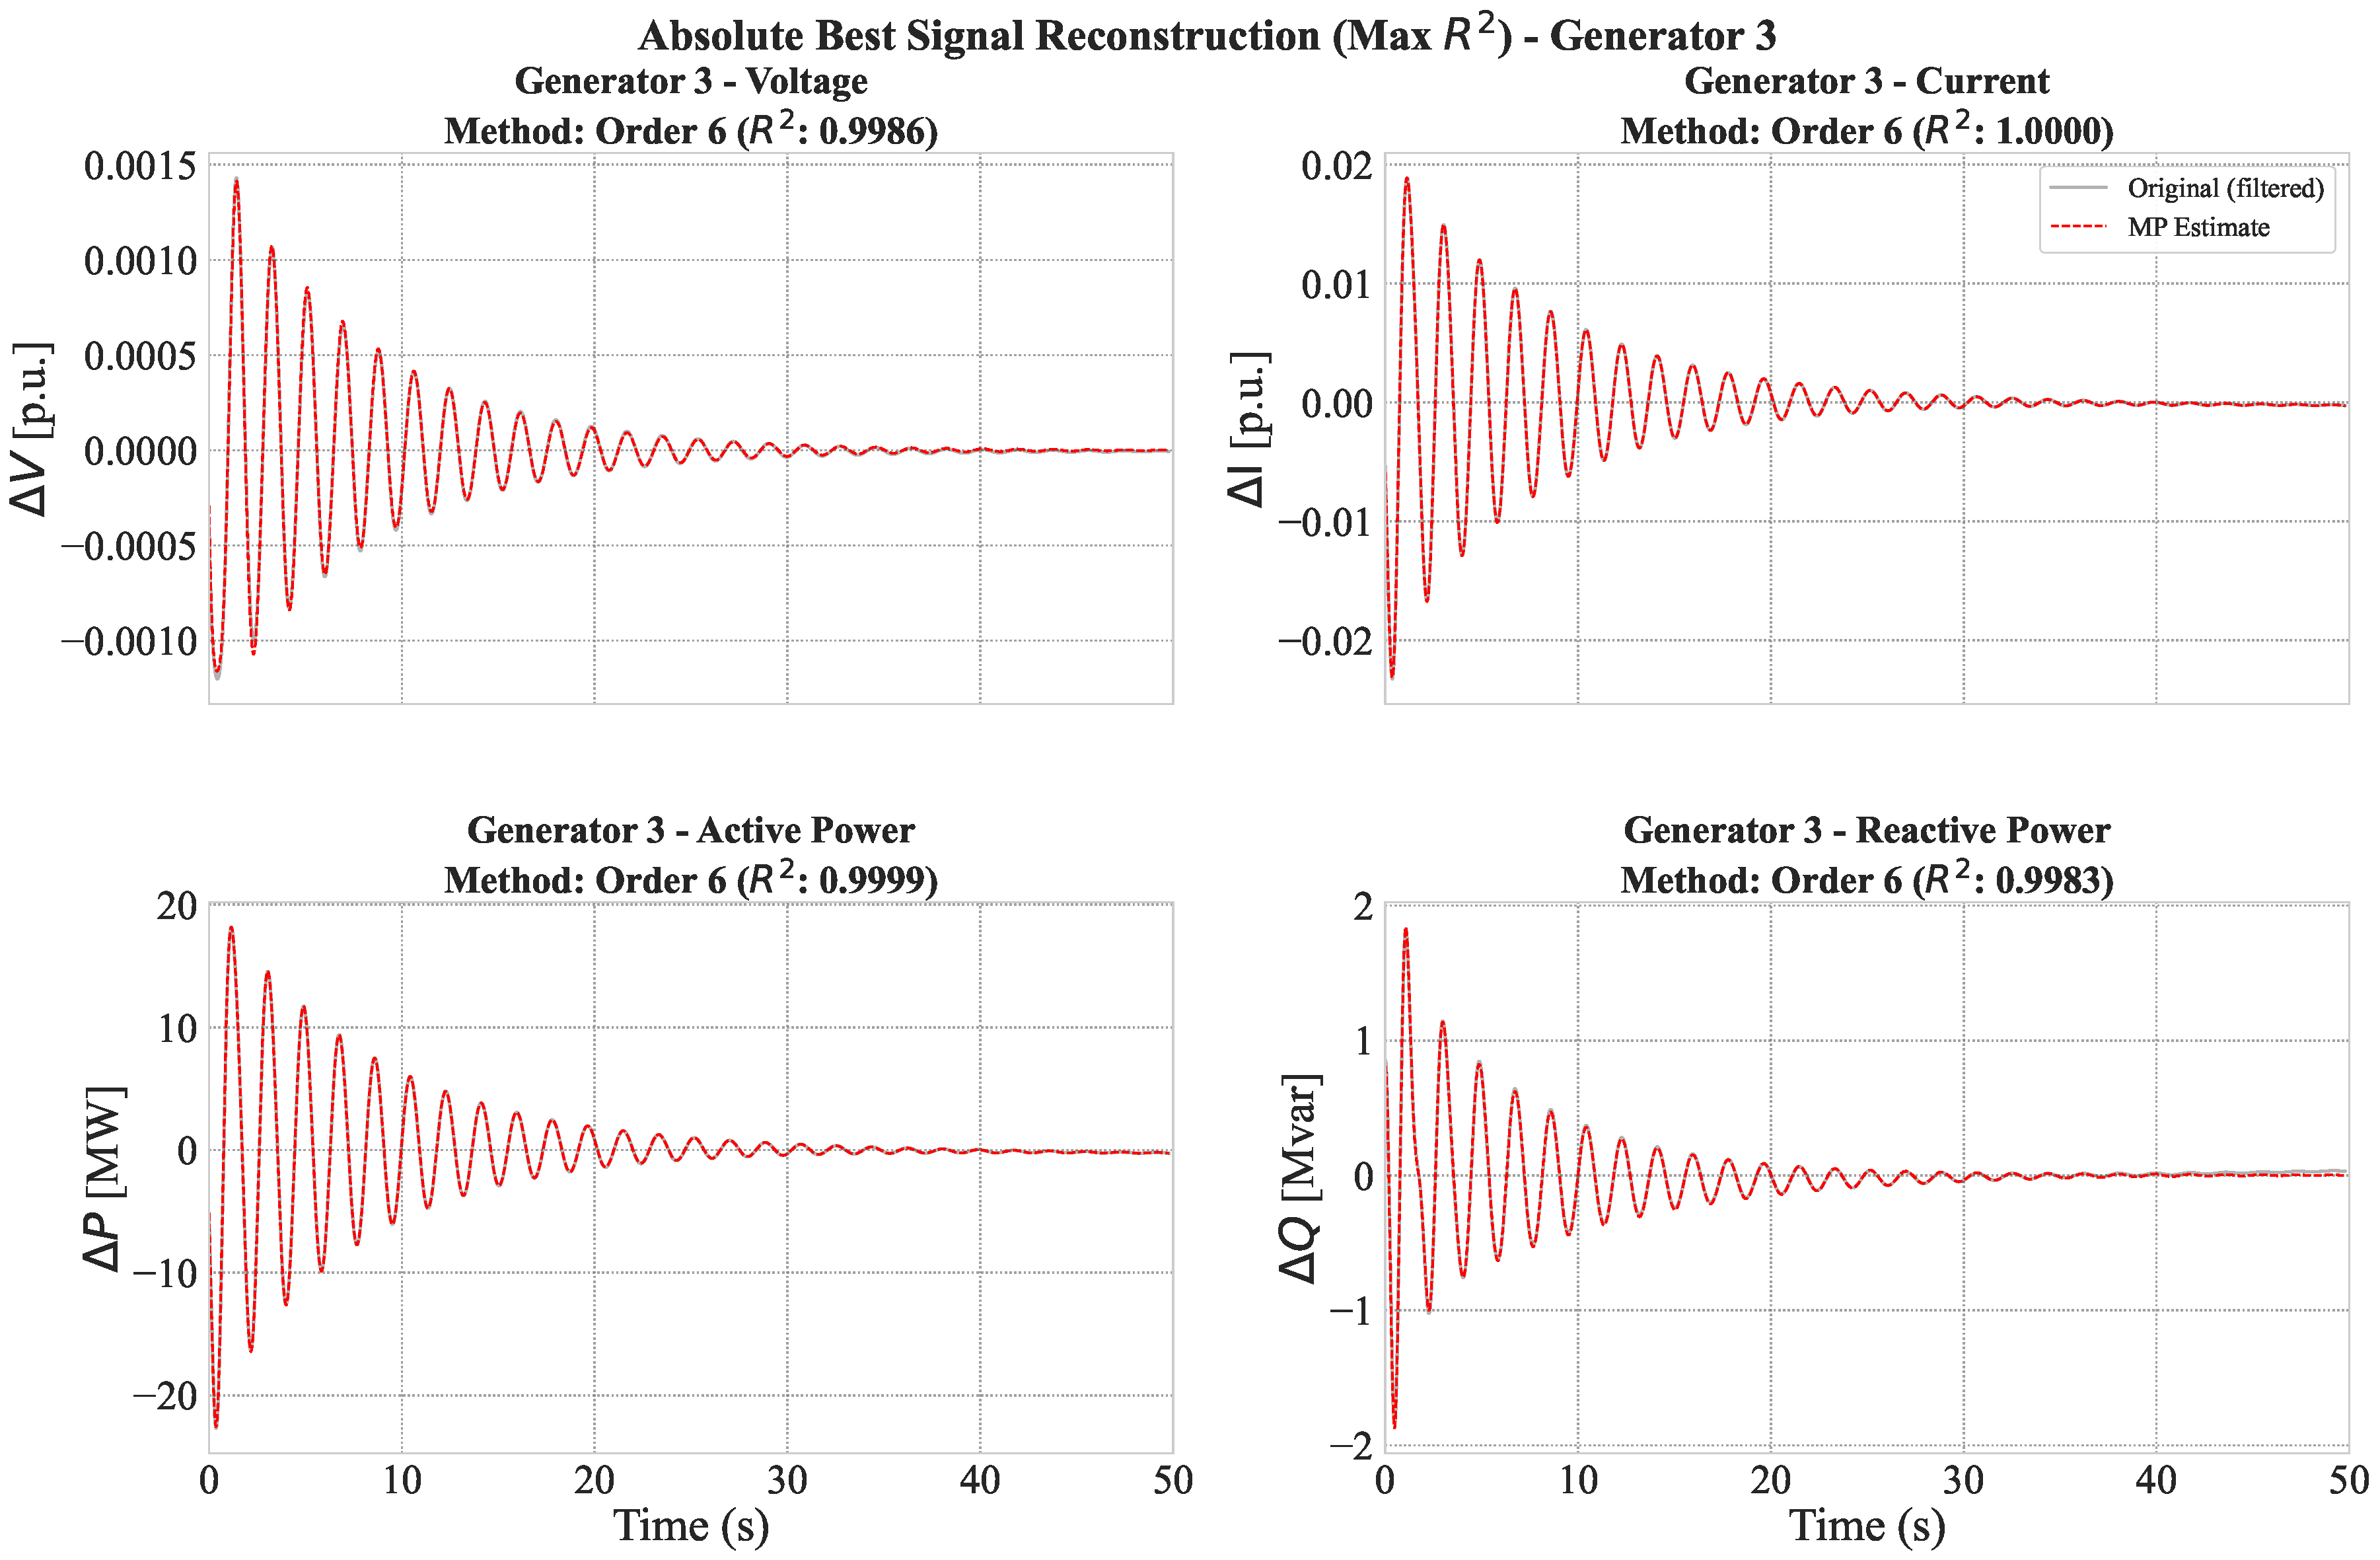
\includegraphics[width=0.95\linewidth]{./stats/pdf/10_best_reconstruction_g3_2x2.pdf} 
    \caption{Βέλτιστη μαθηματική ανακατασκευή των σημάτων ($V, I, P, Q$) για τη γεννήτρια $G_3$ του \textit{Kundur Two-Area System} με βάση τον μέγιστο συντελεστή προσδιορισμού $R^2$.}
    \label{fig:best_recon_g3_kundur}
\end{figure}

\begin{figure}[htbp]
    \centering
    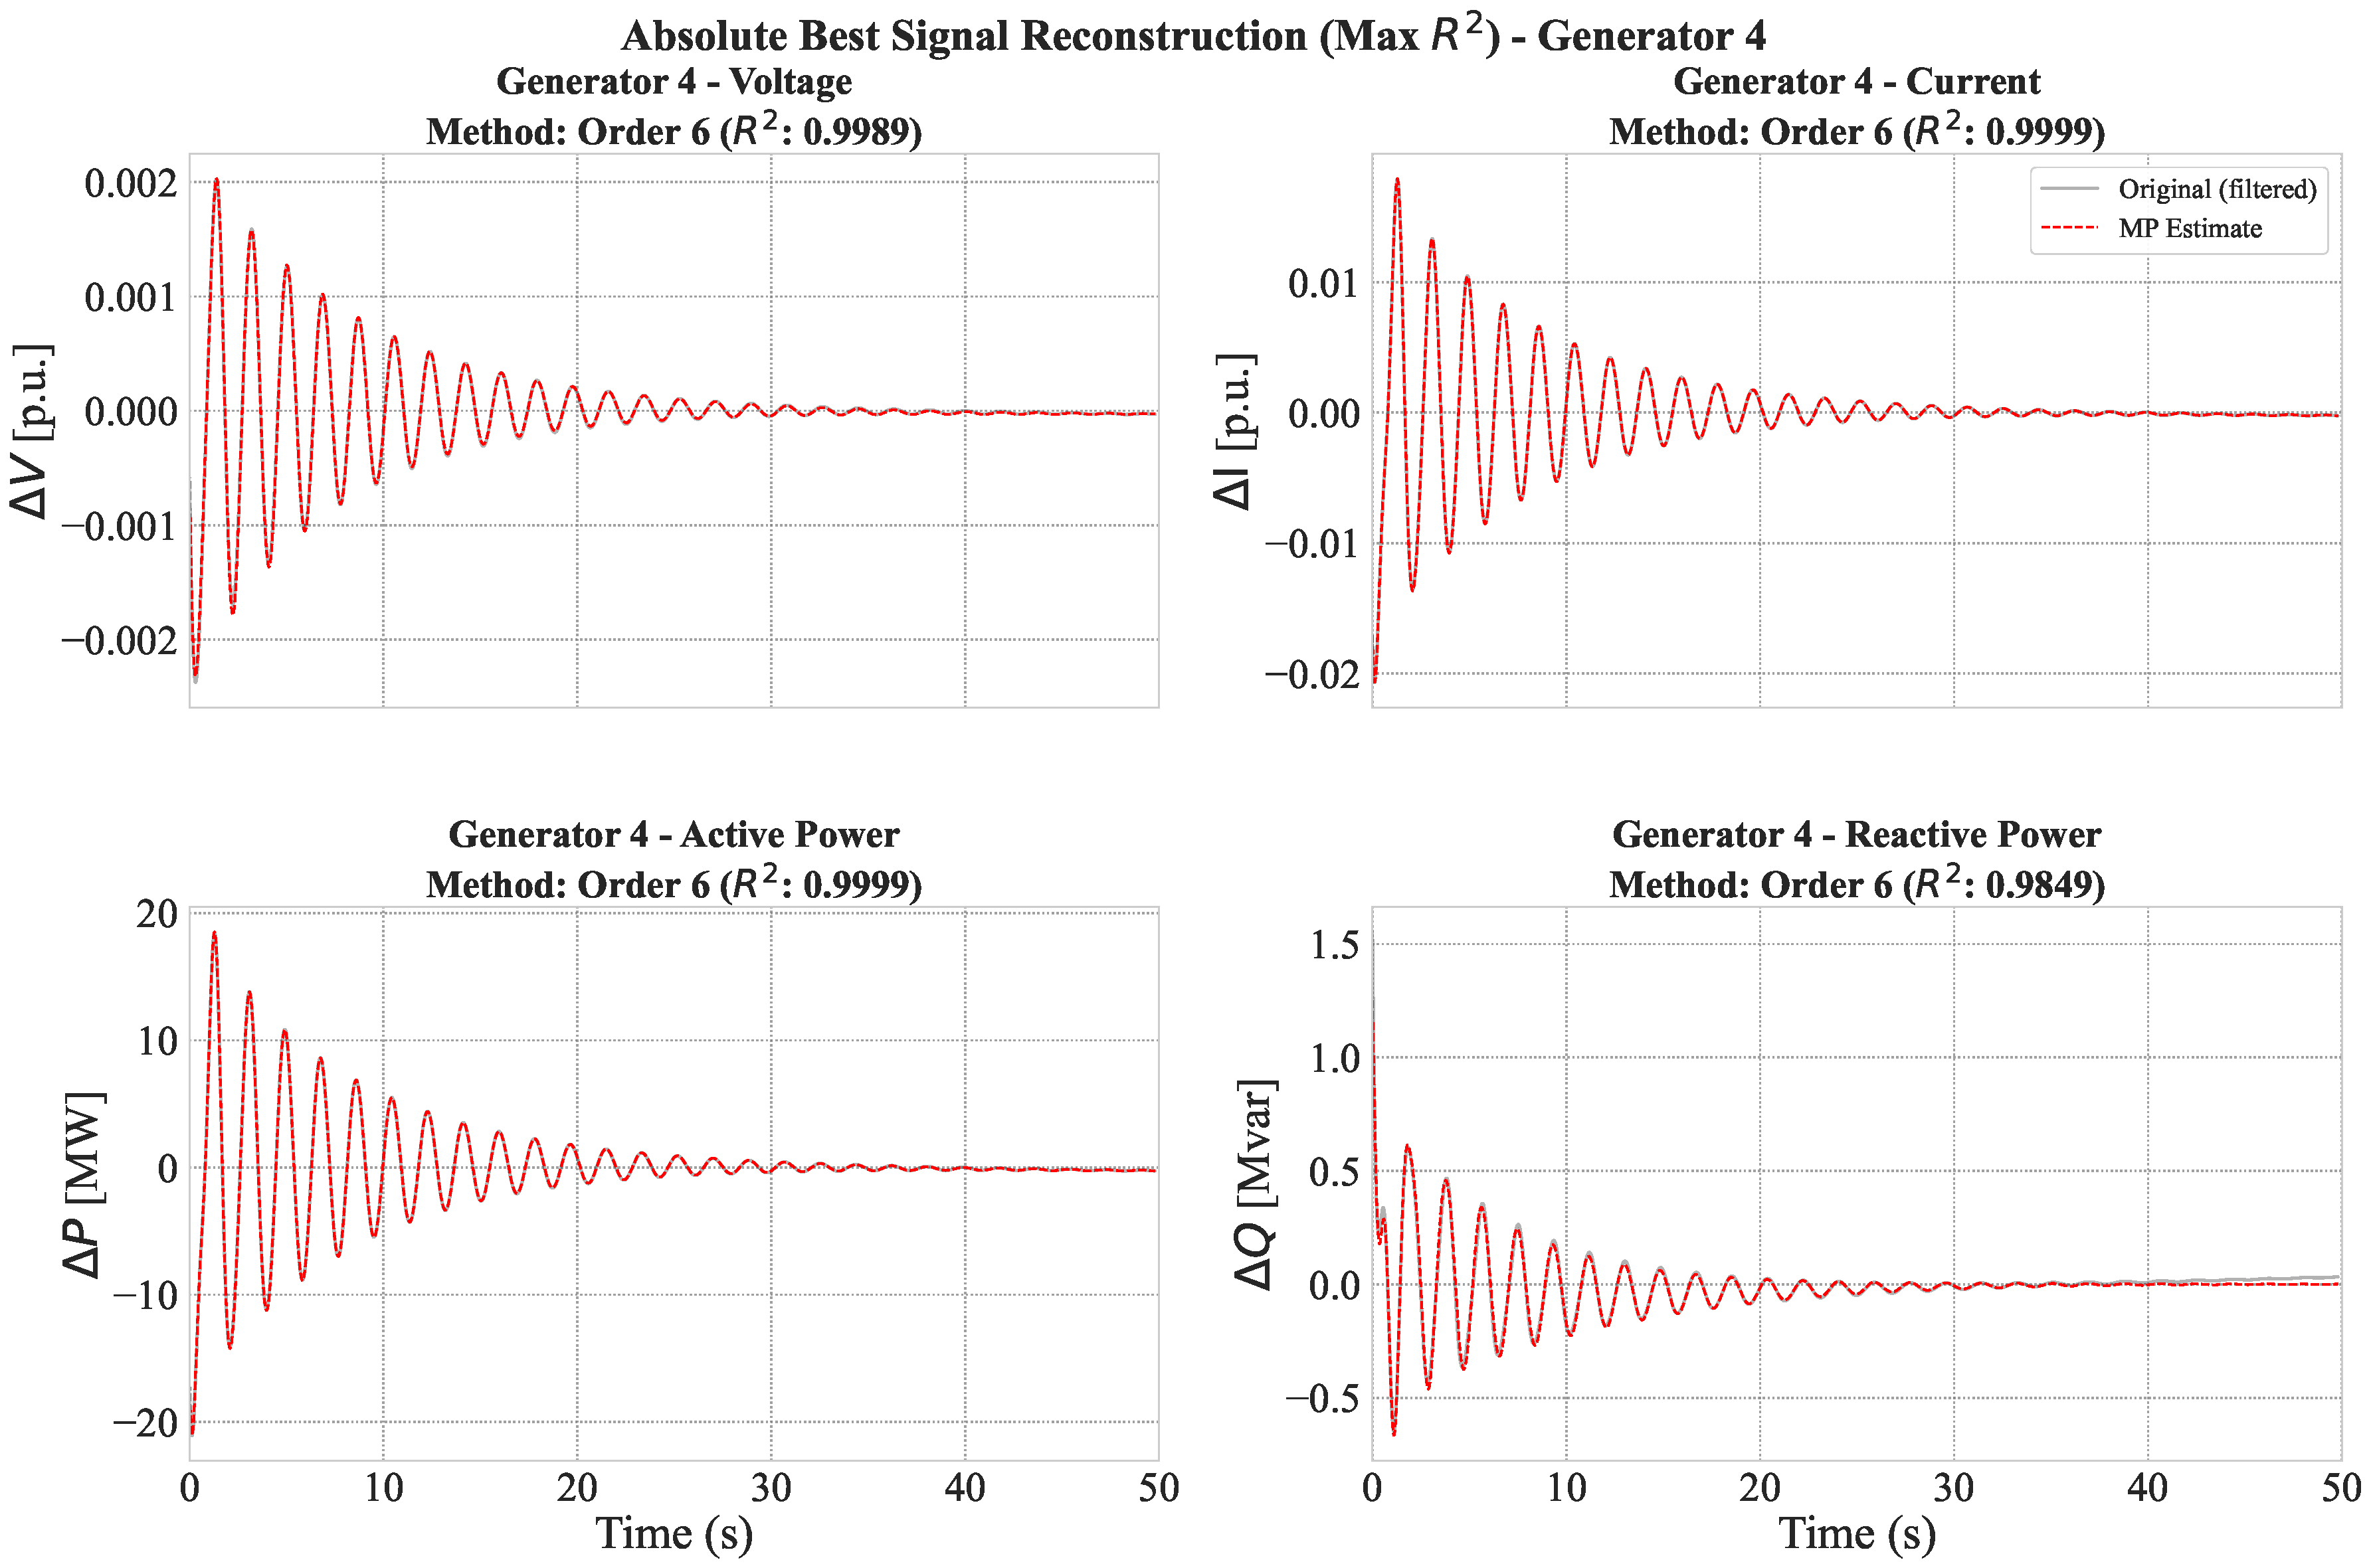
\includegraphics[width=0.95\linewidth]{./stats/pdf/10_best_reconstruction_g4_2x2.pdf} 
    \caption{Βέλτιστη μαθηματική ανακατασκευή των σημάτων ($V, I, P, Q$) για τη γεννήτρια $G_4$ του \textit{Kundur Two-Area System} με βάση τον μέγιστο συντελεστή προσδιορισμού $R^2$.}
    \label{fig:best_recon_g4_kundur}
\end{figure}

\begin{figure}[htbp]
    \centering
    \includegraphics[width=0.95\linewidth]{../IEEE39/analysis/Load03_Pplus2_50s_0.2_to_end_reset/stats/png/10_best_reconstruction_g9_2x2.png} 
    \caption{Βέλτιστη μαθηματική ανακατασκευή των σημάτων ($V, I, P, Q$) για τη γεννήτρια $G_{9}$ του \textit{IEEE 39-Bus System} με βάση τον μέγιστο συντελεστή προσδιορισμού $R^2$.}
    \label{fig:best_recon_g9_ieee39}
\end{figure}

\begin{figure}[htbp]
    \centering
    
\includegraphics[width=0.95\linewidth]{../IEEE39/analysis/Load03_Pplus2_50s_0.2_to_end_reset/stats/png/10_best_reconstruction_g3_2x2.png}
    \caption{Βέλτιστη μαθηματική ανακατασκευή των σημάτων ($V, I, P, Q$) για τη γεννήτρια $G_3$ του \textit{IEEE 39-Bus System} με βάση τον μέγιστο συντελεστή προσδιορισμού $R^2$.}
    \label{fig:best_recon_g3_ieee39}
\end{figure}

\begin{figure}[htbp]
    \centering
    \includegraphics[width=0.95\linewidth]{../IEEE39/analysis/Load03_Pplus2_50s_0.2_to_end_reset/stats/png/10_best_reconstruction_g6_2x2.png}
    \caption{Βέλτιστη μαθηματική ανακατασκευή των σημάτων ($V, I, P, Q$) για τη γεννήτρια $G_6$ του \textit{IEEE 39-Bus System} με βάση τον μέγιστο συντελεστή προσδιορισμού $R^2$.}
    \label{fig:best_recon_g6_ieee39}
\end{figure}

Όπως παρατηρείται, επιτυγχάνεται εξαιρετική σύμπτωση των δύο κυματομορφών σε όλες τις εξεταζόμενες γεννήτριες, ωστόσο αξίζει να σημειωθεί ότι η βέλτιστη ανακατασκευή δεν προκύπτει από μία καθολική μέθοδο γεγονός που επιβεβαιώνει την αναγκαιότητα εξέτασης πολλαπλών προσεγγίσεων.

Τέλος, η ταύτιση των κυματομορφών αναλύεται στο χρονικό παράθυρο της ελεύθερης ταλάντωσης (\textit{ringdown}) για $ t> 0.2$ s. Η υψηλή πιστότητα της ανακατασκευής επιβεβαιώνει την ορθή επιλογή του παραθύρου ανάλυσης, καθώς και την αποτελεσματικότητα της προεπεξεργασίας των σημάτων.
\subsection{Ταυτοποίηση Κυρίαρχων Ταλαντώσεων (Συνολική Αξιολόγηση)}
\label{subsec:overall_evaluation}

Η συνολική αξιολόγηση της δυναμικής του συστήματος πραγματοποιήθηκε με βάση τα διαγράμματα της Ενότητας \ref{sec:modal_and_reconstruction_plots} και τους Χάρτες Ιδιοτιμών (\textit{Bubble Maps}) των Figures \ref{fig:bubble_map_kundur} και \ref{fig:bubble_map_ieee39}. Με τον τρόπο αυτό αποτυπώθηκαν συνολικά η συχνότητα, η απόσβεση και η ενέργεια των ταυτοποιημένων ρυθμών ταλάντωσης.
Για την αποτύπωση της σχετικής σημασίας κάθε ταλαντωτικού ρυθμού στους Χάρτες Ιδιοτιμών, υπολογίστηκε η ενέργεια κάθε ιδιοτιμής σύμφωνα με:
\begin{equation}
\omega_i = 2\pi f_i
\end{equation}
\begin{equation}
\label{eq:pole_energy}
E_i = \frac{1}{2}\omega_i^2 \alpha_i^2
\end{equation}
όπου $f_i$ είναι η συχνότητα και $\alpha_i$ το πλάτος του $i$-οστού ρυθμού. Το μέγεθος κάθε φυσαλίδας στα Figures \ref{fig:bubble_map_kundur} και \ref{fig:bubble_map_ieee39} είναι ανάλογο της ποσότητας $E_i$ \cite{sfetkos2024measurement}.

Η συγκεκριμένη απεικόνιση παρέχει τη συνολικότερη εικόνα της ταυτοποίησης και επιβεβαιώνει τα ευρήματα που παρουσιάστηκαν στην Ενότητα \ref{sec:modal_and_reconstruction_plots}. Παρατηρείται συγκέντρωση ιδιοτιμών σε τρεις βασικές περιοχές συχνοτήτων: πολύ κοντά στο $0$ Hz, στην περιοχή $0.5$--$0.6$ Hz και γύρω από το $1.1$ Hz. Η πρώτη περιοχή συνδέεται κυρίως με αργές μη ταλαντωτικές συνιστώσες και με αριθμητικά artifacts της μεθόδου, ενώ οι υπόλοιπες αντιστοιχούν σε κυρίαρχους ταλαντωτικούς ρυθμούς του συστήματος. Παράλληλα, η κατανομή των ιδιοτιμών ως προς τον ρυθμό απόσβεσης $\sigma$ δείχνει ότι οι ταλαντώσεις εμφανίζουν γενικά θετική απόσβεση, καθώς τα περισσότερα σημεία εντοπίζονται στο αριστερό ημιεπίπεδο.

\begin{figure}[htbp]
    \centering
    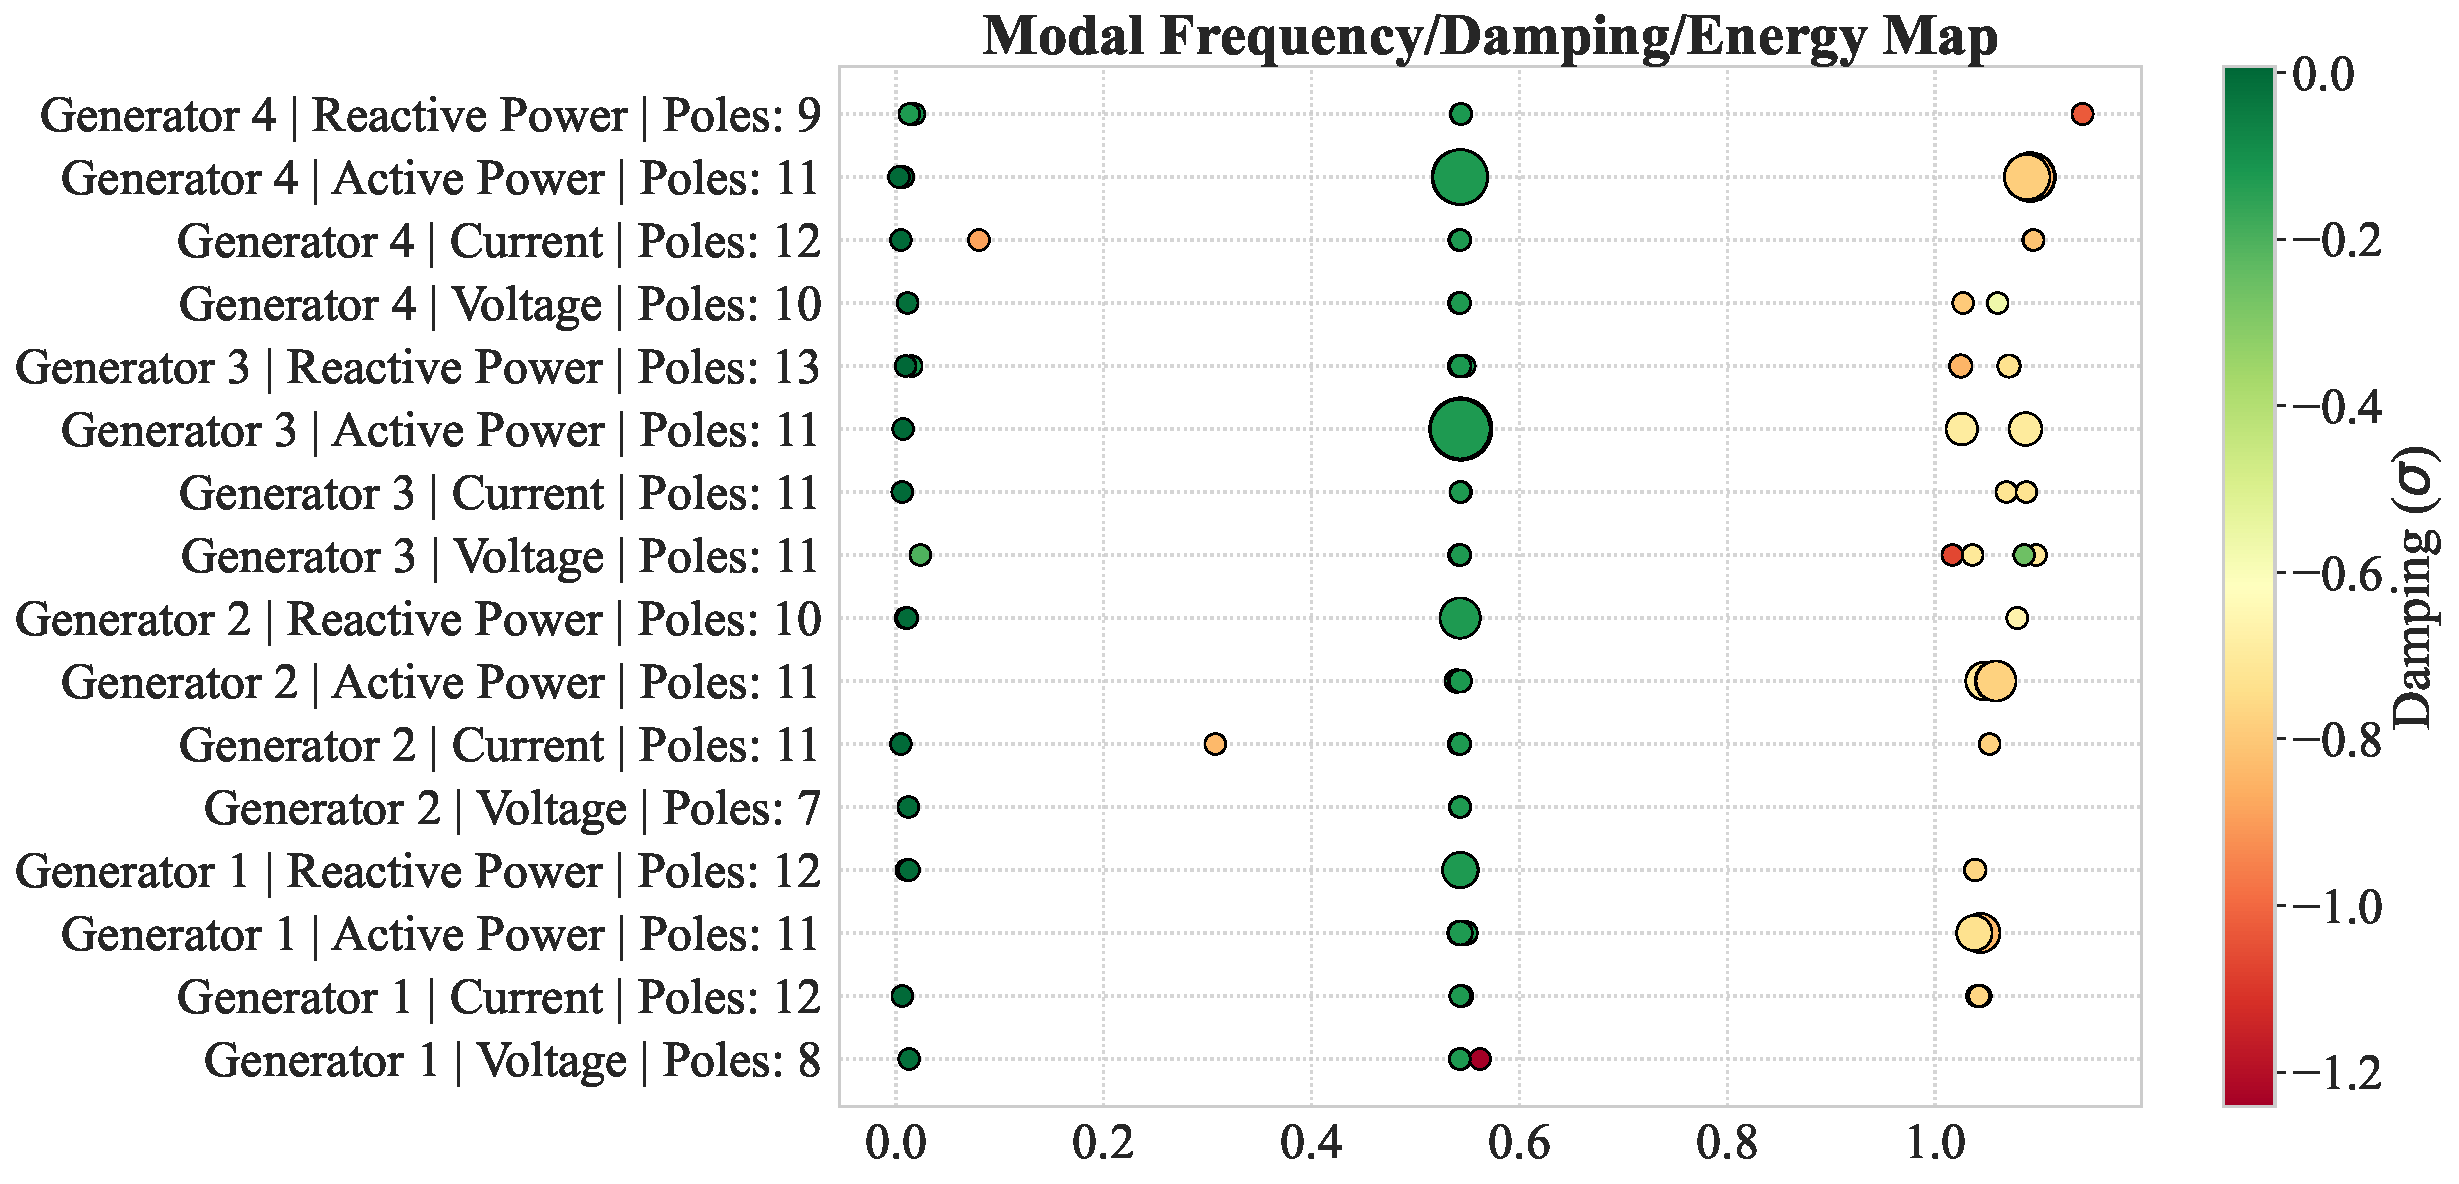
\includegraphics[width=0.95\linewidth]{./stats/pdf/5_bubble_map.pdf}
    \caption{Χάρτης Ιδιοτιμών (\textit{Bubble Map}): Συγκεντρωτική απεικόνιση συχνότητας, απόσβεσης και ενέργειας των ταυτοποιημένων \textit{modes}.}
    \label{fig:bubble_map_kundur}
\end{figure}

\begin{figure}[htbp]
    \centering
    \includegraphics[width=0.95\linewidth]{../IEEE39/analysis/Load03_Pplus2_50s_0.2_to_end_reset/stats/pdf/5_bubble_map_single_panel.pdf}
    \caption{Χάρτης Ιδιοτιμών (\textit{Bubble Map}): Συγκεντρωτική απεικόνιση συχνότητας, απόσβεσης και ενέργειας των ταυτοποιημένων \textit{modes}.}
    \label{fig:bubble_map_ieee39}
\end{figure}


Για το \textit{Kundur Two-Area System}, η ποσοτική αποτύπωση των κυρίαρχων ιδιοτιμών παρουσιάζεται στον Πίνακα~\ref{tab:summary_modes}. Οι τιμές του πίνακα επιλέχθηκαν με βάση τη μέγιστη ενέργεια στις περιοχές συχνοτήτων $0.4$--$0.6$~Hz και $1.0$--$1.1$~Hz, σύμφωνα με τη σχέση~\ref{eq:pole_energy}. Παρατηρείται σταθερή εμφάνιση συχνοτήτων κοντά στα $0.54$~Hz, οι οποίες αντιστοιχούν στον κυρίαρχο διασυνδετικό ρυθμό (\textit{inter-area mode}) του συστήματος. Αντίστοιχα, στην περιοχή $1.0$--$1.1$~Hz καταγράφονται οι τοπικοί ταλαντωτικοί ρυθμοί (\textit{intra-area modes}), οι οποίοι εμφανίζονται με μεγαλύτερες απόλυτες τιμές απόσβεσης. Αξίζει να σημειωθεί ότι στο \textit{IEEE 39-Bus System} η αντίστοιχη ποσοτική ερμηνεία δεν είναι εξίσου άμεση, λόγω της μεγαλύτερης  πολυπλοκότητας του συστήματος. Για τον λόγο αυτό, η αξιολόγηση του \textit{IEEE 39-Bus System} βασίζεται κυρίως στις συνολικές γραφικές απεικονίσεις και στη συγκριτική ερμηνεία των αποτελεσμάτων.

\begin{table}[h]
\centering
\caption{\textsc{Σύνοψη Κυρίαρχων Ιδιοτιμών με Κριτήριο τη Μέγιστη Ενέργεια}}
\label{tab:summary_modes}
\scriptsize
\setlength{\tabcolsep}{5pt}
\renewcommand{\arraystretch}{1.15}
\begin{tabular}{lccc | lcc}
\toprule
\multicolumn{4}{c}{\textbf{Inter-area Mode ($0.4$--$0.6$ Hz)}} & \multicolumn{3}{c}{\textbf{Intra-area Modes ($1.0$--$1.1$ Hz)}} \\
\cmidrule(lr){1-4}\cmidrule(lr){5-7}
\textbf{Gen} & \textbf{Signal} & \textbf{$f$ [Hz]} & \textbf{$\sigma$ [rad/s]} & \textbf{Signal} & \textbf{$f$ [Hz]} & \textbf{$\sigma$ [rad/s]} \\
\midrule
    G1 & P & 0.543 & -0.125 & P & 1.043 & -0.838 \\
    & Q & 0.543 & -0.126 & Q & 1.038 & -0.766 \\
    & V & 0.542 & -0.131 & V & -- & -- \\
    & I & 0.543 & -0.125 & I & 1.040 & -0.799 \\
    \midrule
    G2 & P & 0.539 & -0.144 & P & 1.059 & -0.773 \\
    & Q & 0.543 & -0.127 & Q & 1.079 & -0.664 \\
    & V & 0.543 & -0.129 & V & -- & -- \\
    & I & 0.543 & -0.126 & I & 1.052 & -0.776 \\
    \midrule
    G3 & P & 0.544 & -0.136 & P & 1.087 & -0.697 \\
    & Q & 0.543 & -0.124 & Q & 1.025 & -0.848 \\
    & V & 0.543 & -0.130 & V & 1.017 & -1.066 \\
    & I & 0.544 & -0.137 & I & 1.088 & -0.727 \\
    \midrule
    G4 & P & 0.543 & -0.127 & P & 1.091 & -0.849 \\
    & Q & 0.543 & -0.131 & Q & -- & -- \\
    & V & 0.543 & -0.130 & V & 1.027 & -0.796 \\
    & I & 0.543 & -0.127 & I & 1.094 & -0.817 \\
\bottomrule
\end{tabular}
\end{table}

\subsection{Αξιολόγηση των εκτιμήσεων μέσω του δείκτη MAD}
\label{subsec:mad_evaluation}

Μετά το στάδιο ελέγχου και φιλτραρίσματος των δεδομένων, πραγματοποιήθηκε ποσοτική
αξιολόγηση των εκτιμήσεων ιδιοτιμών που προέκυψαν από τη μέθοδο \textit{Matrix Pencil} ως προς
τις θεωρητικές ιδιοτιμές των εξεταζόμενων συστημάτων. Για τον σκοπό αυτό χρησιμοποιήθηκε
ο δείκτης \textit{Median Absolute Deviation (MAD)}~\cite{modal2018}.

\begin{equation}
\mathrm{MAD}_i = \mathrm{median}\left(\left| \hat{\lambda}_{i,j} - \lambda_i \right|\right)
\label{eq:mad_definition}
\end{equation}
όπου \(\hat{\lambda}_{i,j}\) είναι η \(j\)-οστή εκτίμηση της ιδιοτιμής του \(i\)-οστού
mode και \(\lambda_i\) η αντίστοιχη θεωρητική ιδιοτιμή αναφοράς. 

Ως ιδιοτιμές αναφοράς για το \textit{Kundur Two-Area System} λήφθηκαν οι τρεις κυρίαρχες ταλαντωτικές ιδιοτιμές του
συστήματος Kundur~\cite{estimation2021}, οι οποίες παρουσιάζονται στον
Πίνακα~\ref{tab:kundur_reference_modes}. Το πρώτο mode αντιστοιχούσε στο \textit{inter-area}
mode του συστήματος, ενώ τα δύο επόμενα στα \textit{intra-area} modes των δύο περιοχών.
Για το \textit{IEEE 39-Bus System}, ως ιδιοτιμές αναφοράς λήφθηκαν οι εννέα 
ιδιοτιμές που παρουσιάζoνται στον Πίνακα~\ref{tab:ieee39_reference_modes}~\cite{sarkar2024drga}.


\begin{table}[!htbp]
\centering
\caption{\textsc{Ιδιοτιμές αναφοράς του συστήματος Kundur Two-Area System.}}
\label{tab:kundur_reference_modes}
\small
\renewcommand{\arraystretch}{1.2}
\setlength{\tabcolsep}{14pt}
\begin{tabular}{lcc}
\toprule
\textbf{Mode} & \textbf{$f$ [Hz]} & \textbf{$\sigma$ [rad/s]} \\
\midrule
\textit{Inter-area}   & 0.540 & -0.127 \\
\textit{Intra-area} 1 & 1.083 & -0.603 \\
\textit{Intra-area} 2 & 1.119 & -0.631 \\
\bottomrule
\end{tabular}
\end{table}

\begin{table}[!htbp]
\centering
\caption{\textsc{Ιδιοτιμές αναφοράς του συστήματος IEEE 39-Bus.}}
\label{tab:ieee39_reference_modes}
\scriptsize
\renewcommand{\arraystretch}{1.15}
\setlength{\tabcolsep}{5pt}
\begin{tabular}{lccccc}
\toprule
\textbf{Mode} & \textbf{$f$ [Hz]} & \textbf{$\sigma$ [rad/s]}  & \textbf{Generators} & \textbf{Areas} & \textbf{Type} \\
\midrule
Mode 1 & 0.6062 & -0.0800  & 1--9 vs. 10 & 1-3 &  Inter-area\\
Mode 2 & 0.9497 & -0.1065  & 1, 8, 9 vs. 4, 5, 6, 7 & 1, 2 & Inter-area \\
Mode 3 & 1.0312 & -0.2558  & 2, 3 vs. 4, 5 & 2, 3 & Inter-area\\
Mode 4 & 1.1211 & -0.3373  & 2, 3 vs. 6, 7 &  2, 3 & Inter-area \\
Mode 5 & 1.3155 & -0.4033  & 2 vs. 3 &  2 & Intra-area\\
Mode 6 & 1.2851 & -0.3458  & 1 vs. 8, 9 & 1 & Intra-area\\
Mode 7 & 1.4953 & -0.7033  & 4 vs. 5 & 3 & Intra-area\\
Mode 8 & 1.5202 & -0.6010  & 5, 7 vs. 4, 6 & 3 & Intra-area\\
Mode 9 & 1.5468 & -0.6376  & 1 vs. 8 & 1 & Intra-area\\
\bottomrule
\end{tabular}
\end{table}

Για τον υπολογισμό του MAD χρησιμοποιήθηκαν οι εκτιμήσεις που παρέμειναν μετά το
στάδιο ελέγχου δεδομένων της Παραγράφου~\ref{subsec:data_screening}. Στη συνέχεια,
κάθε εκτιμώμενη ιδιοτιμή αντιστοιχίστηκε στο πλησιέστερο mode αναφοράς με κριτήριο την
Ευκλείδεια απόσταση στο επίπεδο συχνότητας--απόσβεσης $(f,\sigma)$. Με τον τρόπο
αυτό, ο δείκτης MAD παρείχε ένα συνοπτικό και ανθεκτικό μέτρο της απόκλισης των τελικών
εκτιμήσεων από τις θεωρητικές θέσεις των κυρίαρχων ταλαντωτικών ρυθμών του συστήματος.

Τα βασικά αποτελέσματα των υπολογισμών συνοψίζονται στα Tables~\ref{tab:mad_summary_kundur} και ~\ref{tab:mad_summary_ieee39}, όπου παρουσιάζονται, για κάθε mode αναφοράς, το
πλήθος των εκτιμήσεων που αντιστοιχίστηκαν σε αυτό, η τιμή του MAD, καθώς και οι αντίστοιχες τιμές της μέσης και της μέγιστης απόστασης των εκτιμήσεων από την ιδιοτιμή αναφοράς.

Τα αποτελέσματα του Πίνακα~\ref{tab:mad_summary_kundur} για το \textit{Kundur Two-Area System} έδειξαν ότι η καλύτερη συμφωνία
με τη θεωρητική ιδιοτιμή αναφοράς παρατηρήθηκε για το \textit{inter-area} mode, για το οποίο
προέκυψαν η μικρότερη τιμή MAD ($0.0036$) και η μικρότερη μέση απόσταση ($0.0125$).
Επιπλέον, στο συγκεκριμένο mode αντιστοιχίστηκε και το μεγαλύτερο πλήθος εκτιμήσεων
($97$), όπως ήταν αναμενόμενο, καθώς το \textit{inter-area} mode είναι γενικά παρατηρήσιμο από
μεγαλύτερο αριθμό γεννητριών και σημάτων του συστήματος σε σύγκριση με τα \textit{intra-area}
modes. Αντίθετα, τα \textit{intra-area} modes παρουσίασαν μεγαλύτερες τιμές MAD και, συνεπώς,
μεγαλύτερη απόκλιση από τις θεωρητικές ιδιοτιμές αναφοράς. Ειδικότερα, το
\textit{Intra-area} mode 2 παρουσίασε τη λιγότερο ικανοποιητική εικόνα, με τιμή MAD ίση με
$0.1573$ και μέση απόσταση $0.1665$, και αντιστοιχίστηκαν $41$
εκτιμήσεις. Το \textit{Intra-area} mode 1 εμφάνισε ενδιάμεση συμπεριφορά, με τιμή MAD ίση με
$0.1047$, μέση απόσταση $0.2719$ και συνολικά $5$ αντιστοιχισμένες εκτιμήσεις.



\begin{table}[!t]
\centering
\caption{\textsc{Συνοπτικά αποτελέσματα του δείκτη \textit{MAD} ανά mode αναφοράς του συστήματος Kundur Two-Area System.}}
\label{tab:mad_summary_kundur}
\small
\renewcommand{\arraystretch}{1.2}
\setlength{\tabcolsep}{8pt}
\begin{tabular}{lcccc}
\toprule
\textbf{Mode} & \textbf{Count} & \textbf{MAD} & \textbf{Mean} & \textbf{Max} \\
\midrule
\textit{Inter-area}   & 97 & 0.0036 & 0.0125 & 0.7470 \\
\textit{Intra-area} 1 & 5  & 0.1047 & 0.2719 & 0.8237 \\
\textit{Intra-area} 2 & 41 & 0.1573 & 0.1665 & 0.4473 \\
\bottomrule
\end{tabular}
\end{table}

Για το \textit{IEEE 39-Bus System}, τα αποτελέσματα του δείκτη MAD παρουσιάζονται στον
Πίνακα~\ref{tab:mad_summary_ieee39} ανά mode αναφοράς. Για modes χωρίς καμία
αντιστοιχισμένη εκτίμηση καταγράφεται πλήθος ίσο με μηδέν. Παρατηρείται ότι η καλύτερη
συμφωνία εμφανίζεται κυρίως για τα Modes~3 και~4, τα οποία παρουσιάζουν τις μικρότερες τιμές MAD
και μέσης απόστασης. Αντίθετα, το Mode~1 συγκεντρώνει το μεγαλύτερο πλήθος εκτιμήσεων ($265$), όπως ήταν αναμενόμενο καθώς είναι παρατηρίσιμο από όλες τις περιοχές ελέγχου του συστήματος, αλλά και σαφώς μεγαλύτερη τιμή δείκτη \textit{MAD} ($0.2638$). Σημειώνεται ότι, για το \textit{IEEE 39-Bus System}, οι εκτιμήσεις κάθε περιοχής ελέγχου αντιστοιχίζονται μόνο στα modes αναφοράς για τα οποία η βιβλιογραφία υποδεικνύει συμμετοχή των αντίστοιχων γεννητριών. Με τον τρόπο αυτό, οι αντιστοιχίσεις των εκτιμήσεων στα reference modes παραμένουν συμβατές με τη φυσική ερμηνεία των ταλαντωτικών μορφών του συστήματος.
Συνολικά, τα αποτελέσματα για το \textit{IEEE 39-Bus System} εμφανίζονται λιγότερο συμπαγή σε σύγκριση με εκείνα του \textit{Kundur Two-Area System}, γεγονός που είναι αναμενόμενο λόγω της σημαντικά μεγαλύτερης πολυπλοκότητας του συστήματος.

\begin{table}[!t]
\centering
\caption{\textsc{Συνοπτικά αποτελέσματα του δείκτη \textit{MAD} για το IEEE 39-Bus ανά mode αναφοράς.}}
\label{tab:mad_summary_ieee39}
\small
\renewcommand{\arraystretch}{1.2}
\setlength{\tabcolsep}{6pt}
\begin{tabular}{lccccc}
\toprule
\textbf{Mode} & \textbf{$f$ [Hz]} & \textbf{Count} & \textbf{MAD} & \textbf{Mean} & \textbf{Max} \\
\midrule
Mode 1 & 0.6062 & 265 & 0.2638 & 0.3609 & 1.2372 \\
Mode 2 & 0.9497 & 2   & 0.1986 & 0.1986 & 0.2043 \\
Mode 3 & 1.0312 & 15  & 0.0575 & 0.0621 & 0.1209 \\
Mode 4 & 1.1211 & 41  & 0.0809 & 0.0880 & 0.3815 \\
Mode 5 & 1.3155 & 0   & --     & --     & --     \\
Mode 6 & 1.2851 & 32  & 0.1817 & 0.2075 & 0.4732 \\
Mode 7 & 1.4953 & 4   & 0.3490 & 0.3521 & 0.5526 \\
Mode 8 & 1.5202 & 0   & --     & --     & --     \\
Mode 9 & 1.5468 & 3   & 0.2954 & 0.3109 & 0.3430 \\
\bottomrule
\end{tabular}
\end{table}

Στη συνέχεια, η ανάλυση συμπληρώθηκε με εφαρμογή τεχνικών συσταδοποίησης στις
εκτιμήσεις ιδιοτιμών, με στόχο τη διερεύνηση της εσωτερικής τους οργάνωσης στο επίπεδο
συχνότητας--απόσβεσης και την ανάδειξη των κυρίαρχων περιοχών συγκέντρωσης.


\subsection{Αποτελέσματα συσταδοποίησης}

Στόχος της συσταδοποίησης ήταν η ομαδοποίηση των ταυτοποιημένων ιδιοτιμών, με σκοπό τον εντοπισμό των κυρίαρχων ρυθμών ταλάντωσης του συστήματος και τη διερεύνηση του κατά πόσο οι διαφορετικές μέθοδοι συσταδοποίησης συγκλίνουν σε κοινές περιοχές συχνοτήτων και αποσβέσεων. Όπως περιγράφηκε προηγουμένως στην παράγραφο \ref{subsec:data_screening}, εφαρμόστηκε φιλτράρισμα των ιδιοτιμών, διατηρώντας μόνο εκείνες με συχνότητες εντός του διαστήματος $[0.1,\,2.0]$~Hz, προκειμένου να διασφαλιστεί ότι οι συστάδες που προκύπτουν αντιστοιχούν σε φυσικούς ρυθμούς ταλάντωσης του συστήματος.

Για τη διερεύνηση της δομής των δεδομένων εφαρμόστηκαν οι αλγόριθμοι συσταδοποίησης \textit{k-Means} και \textit{k-Medoids} για τιμές \(k = 1,2,\ldots,10\). Η επιλογή του βέλτιστου αριθμού συστάδων βασίστηκε σε δύο συμπληρωματικά κριτήρια: τη μέθοδο \textit{Elbow}, για τον εντοπισμό του σημείου καμπής της καμπύλης κόστους, και τη μέθοδο \textit{Silhouette}, για την αξιολόγηση της συνοχής και του διαχωρισμού των συστάδων. Για τον αυτόματο εντοπισμό του σημείου καμπής στο διάγραμμα \textit{Elbow} χρησιμοποιήθηκε η τεχνική \textit{Maximum Chord Distance}.

Ειδικότερα, τα δύο κριτήρια εφαρμόστηκαν ως εξής. Αρχικά εφαρμόστηκε η μέθοδος \textit{Elbow}, η οποία για τον \textit{k-Means} βασίστηκε στο μέτρο WCSS (\textit{Within-Cluster Sum of Squares}), ενώ για τον \textit{k-Medoids} στο συνολικό κόστος (\textit{Total Cost}). Για τον αυτόματο εντοπισμό του σημείου καμπής της αντίστοιχης καμπύλης χρησιμοποιήθηκε η τεχνική \textit{Maximum Chord Distance}, η οποία υπολογίζει την απόσταση κάθε σημείου από την ευθεία που ενώνει το πρώτο και το τελευταίο σημείο της καμπύλης. Το σημείο με τη μέγιστη απόσταση επιλέγεται ως υποψήφιο βέλτιστο \(k\), καθώς πέρα από αυτό η περαιτέρω αύξηση του αριθμού συστάδων οδηγεί σε περιορισμένη μόνο βελτίωση της ποιότητας συσταδοποίησης.

Παράλληλα, χρησιμοποιήθηκε η μέθοδος \textit{Silhouette}, η οποία αξιολογεί την ποιότητα της συσταδοποίησης εξετάζοντας, για κάθε σημείο, τη συνοχή εντός της συστάδας του και τον διαχωρισμό του από τις γειτονικές συστάδες. Η μέση τιμή του \textit{Silhouette Score} χρησιμοποιήθηκε συμπληρωματικά για την επιλογή του βέλτιστου \(k\) και την αποτίμηση της σταθερότητας της ομαδοποίησης.

Η συνδυαστική χρήση των δύο κριτηρίων κρίθηκε σκόπιμη, καθώς η μέθοδος \textit{Elbow} αποτυπώνει κυρίως τη μεταβολή της εσωτερικής συνοχής των συστάδων, ενώ η μέθοδος \textit{Silhouette} παρέχει πρόσθετη πληροφορία για τον βαθμό διαχωρισμού μεταξύ τους. Συνεπώς, η τελική επιλογή του βέλτιστου \(k\) προέκυψε από τη συνεκτίμηση των αντίστοιχων διαγραμμάτων και δεικτών.

\subsubsection{Αποτελέσματα για το \textit{Kundur Two-Area}}
\paragraph{Αποτελέσματα k-Means}

Για τον αλγόριθμο \textit{k-Means}, ο δείκτης WCSS ως συνάρτηση του αριθμού συστάδων παρουσιάζεται στο Figure~\ref{fig:k_means_elbow_kundur}. Η εφαρμογή της τεχνικής \textit{Maximum Chord Distance} οδήγησε στην επιλογή της τιμής $k=2$ ως βέλτιστης, ενώ η ανάλυση με τη μέθοδο \textit{Silhouette} έδειξε ότι η μέση τιμή του \textit{Silhouette Score} μεγιστοποιείται για $k=3$. Ωστόσο, από την εξέταση των αντίστοιχων διαγραμμάτων (Figures~\ref{fig:k_means_2_clusters_kundur} και~\ref{fig:k_means_silhouette_kundur}) προκύπτει ότι η τρίτη συστάδα δεν αντιστοιχεί σε διακριτή ομάδα ιδιοτιμών, αλλά σε περιορισμένο πλήθος απομονωμένων ακραίων σημείων (\textit{outliers}). Για τον λόγο αυτό, η επιλογή του $k=2$ θεωρείται τελικά η πιο αντιπροσωπευτική. Το αποτέλεσμα αυτό είναι συμβατό με τα ευρήματα της Παραγράφου~\ref{subsec:overall_evaluation}, σύμφωνα με τα οποία στο σύστημα Kundur εμφανίζονται ένα \textit{inter-area} mode και δύο \textit{intra-area} modes. Ωστόσο, τα δύο \textit{intra-area} modes είναι πολύ κοντά μεταξύ τους στο επίπεδο συχνότητας και απόσβεσης, με αποτέλεσμα να μην διαχωρίζονται σε δύο σαφώς διακριτές συστάδες και να αποτυπώνονται από τη συσταδοποίηση ως μία ενιαία περιοχή \textit{intra-area} συμπεριφοράς.
\begin{figure}[htbp]
    \centering
    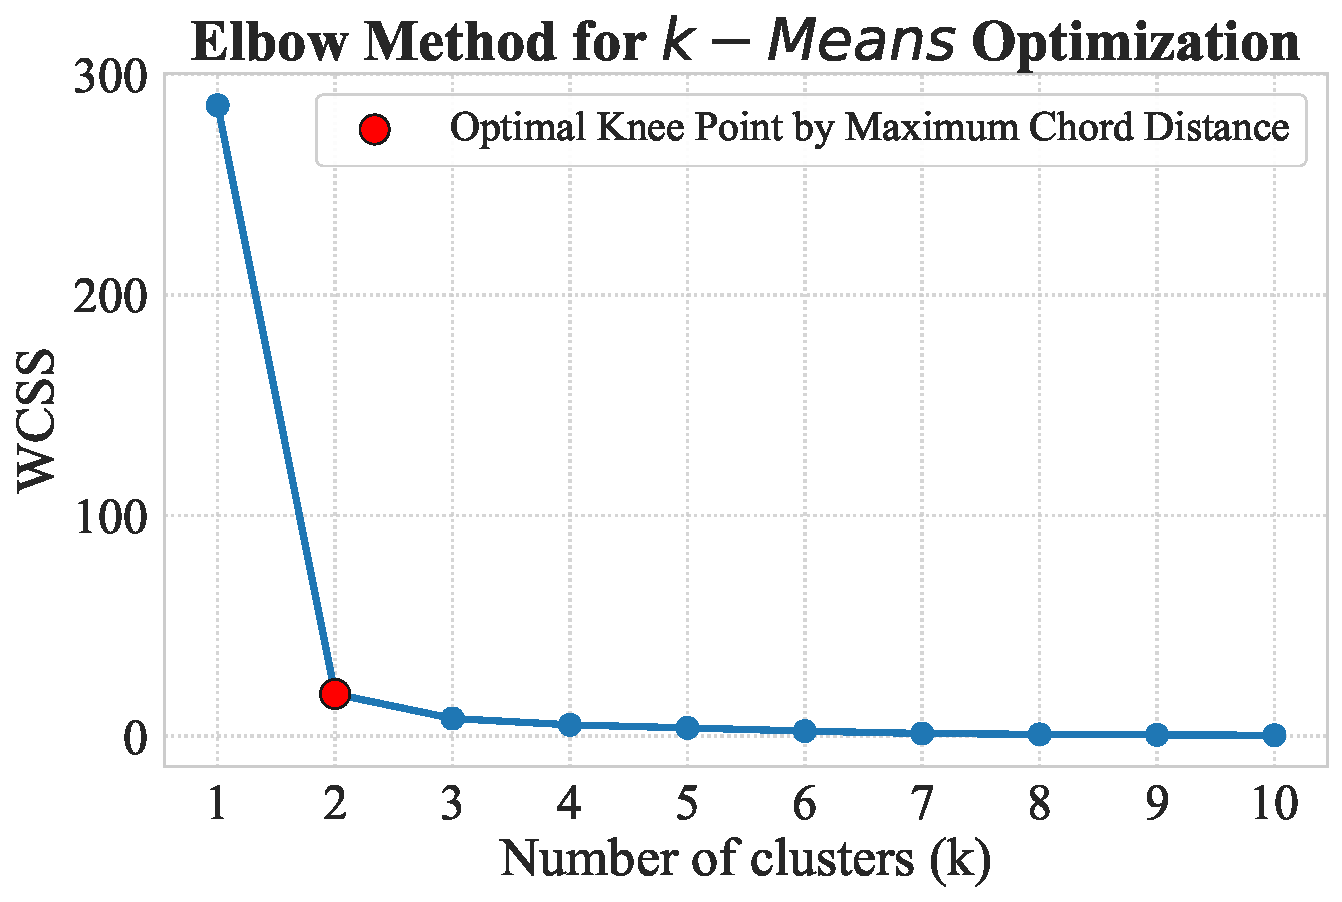
\includegraphics[width=0.95\linewidth]{./clustering/kmeans/pdf/elbow_method.pdf}
    \caption{Διάγραμμα Elbow του αλγορίθμου \textit{k-Means} για το \textit{Kundur Two-Area System}.}
    \label{fig:k_means_elbow_kundur}
\end{figure}

\begin{figure}[htbp]
    \centering
    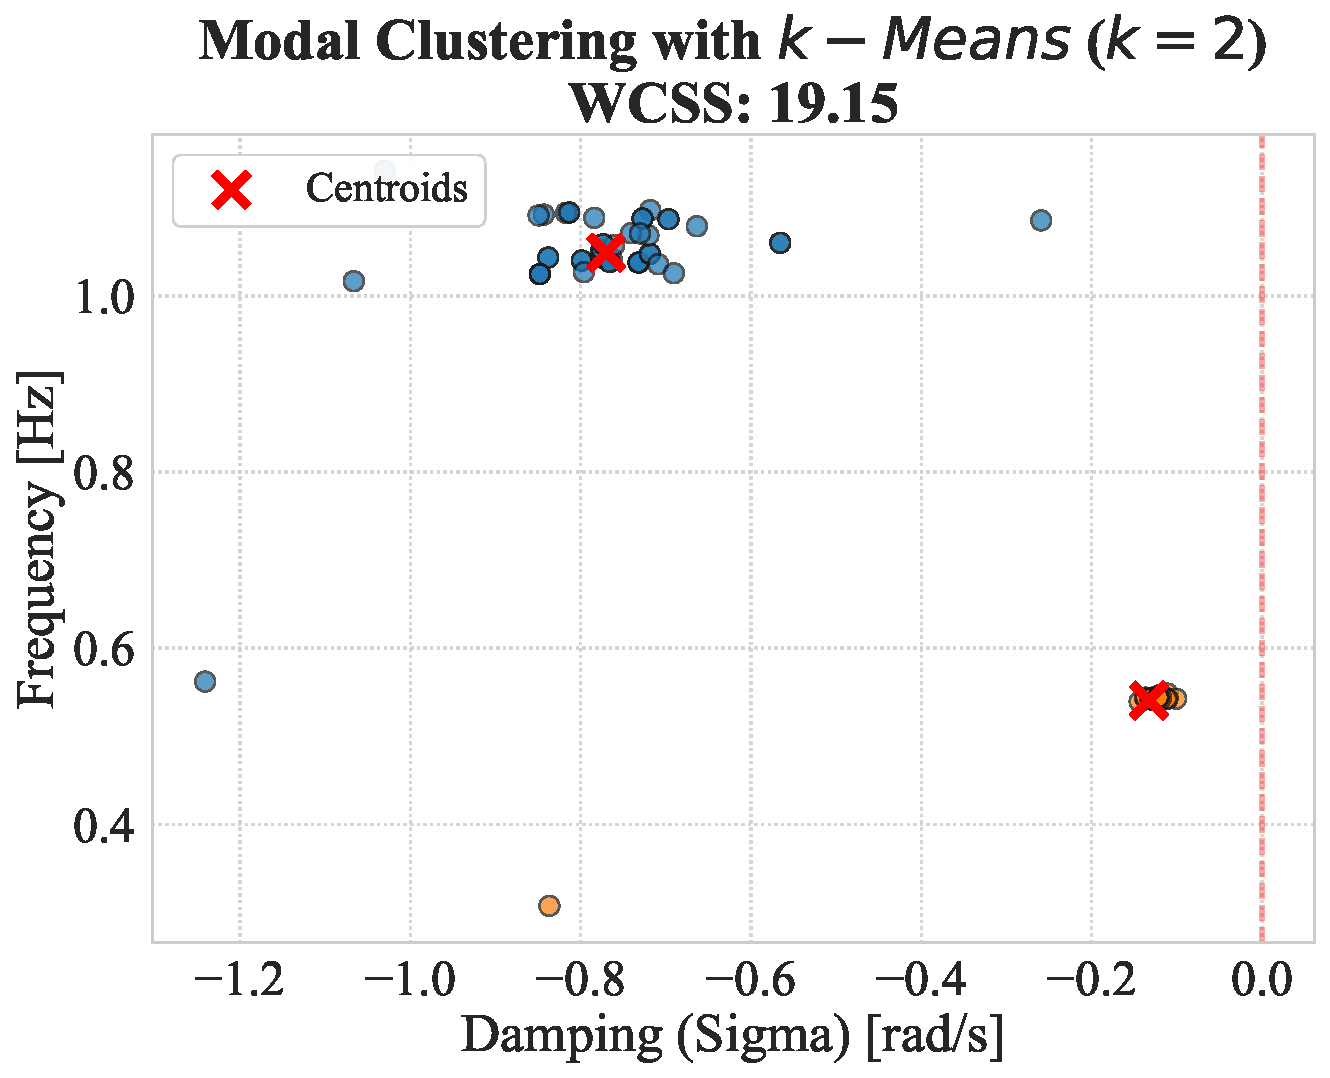
\includegraphics[width=0.95\linewidth]{./clustering/kmeans/pdf/kmeans_modal_map_k2.pdf}
    \caption{Χάρτης ιδιοτιμών του αλγορίθμου \textit{k-Means} για $k=2$ στο \textit{Kundur Two-Area System}.}
    \label{fig:k_means_2_clusters_kundur}
\end{figure}

\begin{figure}[htbp]
    \centering
    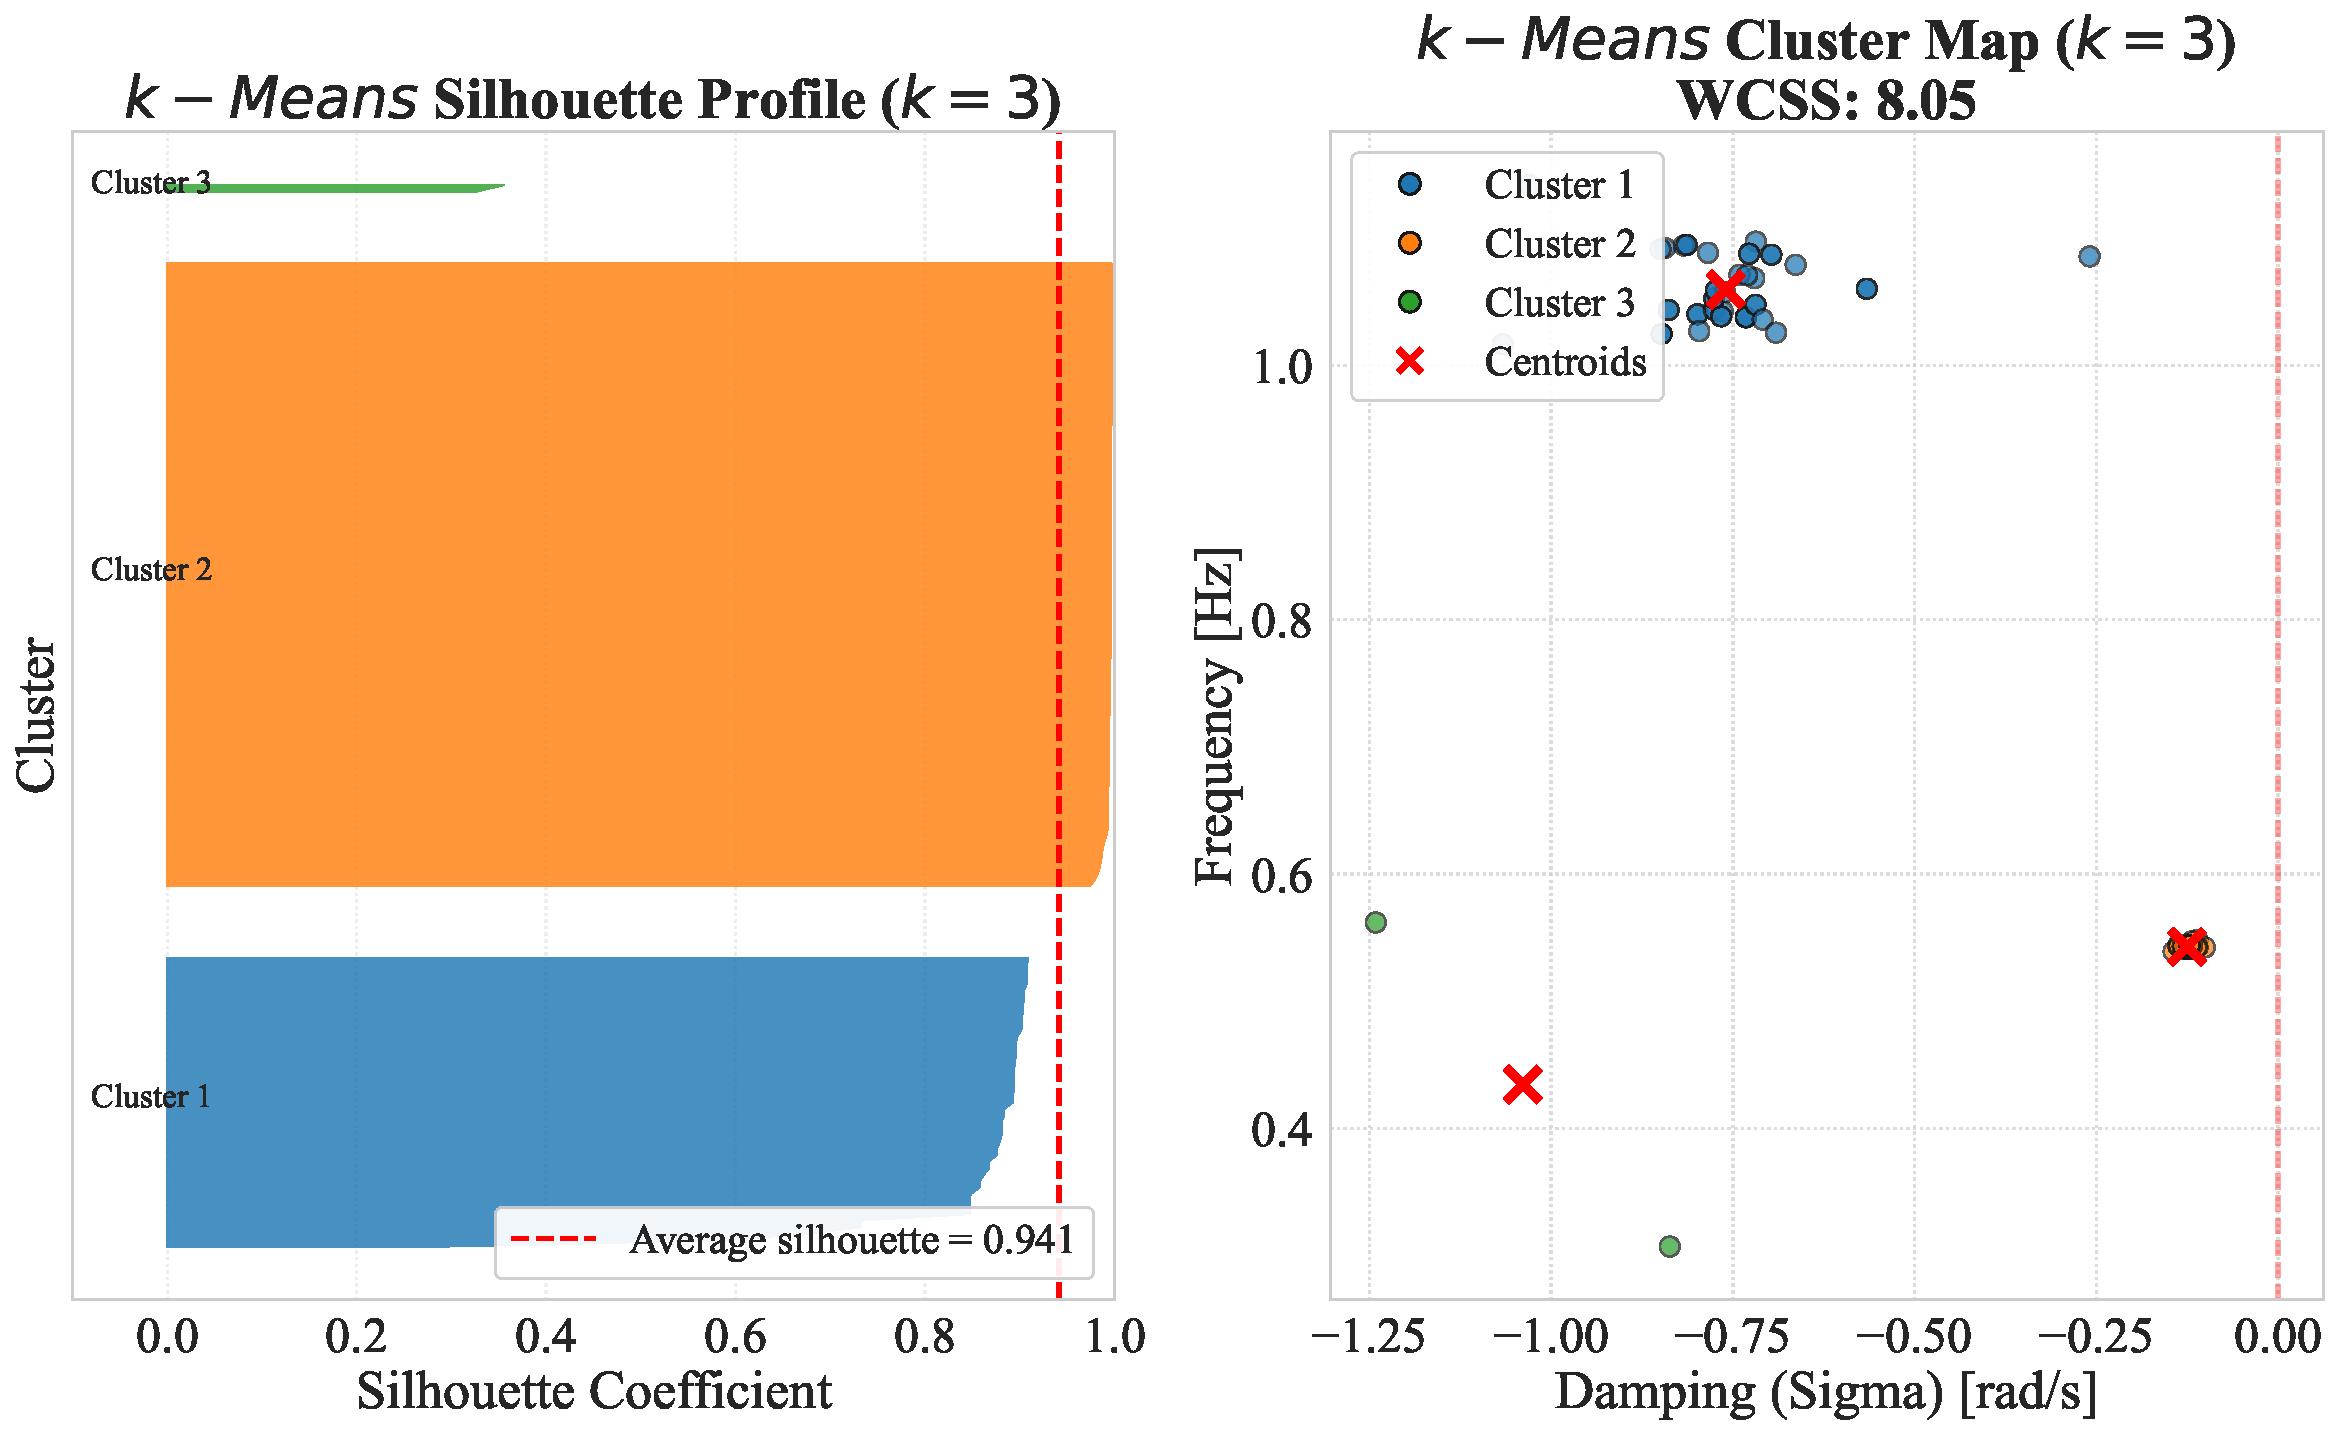
\includegraphics[width=0.95\linewidth]{./clustering/silhouette/pdf/silhouette_profile_kmeans.pdf}
    \caption{Silhouette profile του αλγορίθμου \textit{k-Means} για $k=3$ στο \textit{Kundur Two-Area System}.}
    \label{fig:k_means_silhouette_kundur}
\end{figure}


\paragraph{Αποτελέσματα k-Medoids}

Για τον αλγόριθμο \textit{k-Medoids}, το συνολικό κόστος συσταδοποίησης (\textit{Total Cost}) ως συνάρτηση του αριθμού συστάδων παρουσιάζεται στο Figure~\ref{fig:k_medoids_elbow_kundur}. Το μέγεθος αυτό εκφράζει το άθροισμα των αποστάσεων όλων των ιδιοτιμών από το αντίστοιχο \textit{medoid} της συστάδας τους. Όπως αναμένεται, το συνολικό κόστος μειώνεται όσο αυξάνεται ο αριθμός συστάδων, καθώς η κατανομή των ιδιοτιμών περιγράφεται με μεγαλύτερη λεπτομέρεια. Ωστόσο, η εφαρμογή της τεχνικής \textit{Maximum Chord Distance} οδήγησε στην επιλογή της τιμής $k=2$ ως βέλτιστης, ενώ η ανάλυση με τη μέθοδο \textit{Silhouette} έδειξε ότι η μέση τιμή του \textit{Silhouette Score} μεγιστοποιείται για $k=3$.

Η ερμηνεία των αποτελεσμάτων του \textit{k-Medoids} ακολουθεί την ίδια λογική με εκείνη του \textit{k-Means}. Αν και το \textit{Silhouette Profile} του Figure~\ref{fig:k_medoids_silhouette_kundur} εμφανίζει οριακά μεγαλύτερη μέση τιμή για $k=3$ (\(0.941\), έναντι \(0.932\) για $k=2$), η πρόσθετη τρίτη συστάδα αντιστοιχεί και εδώ σε πολύ μικρό πλήθος απομονωμένων σημείων και δεν αποτυπώνει έναν επιπλέον κυρίαρχο φυσικό ρυθμό ταλάντωσης. Επομένως, με γνώμονα τη φυσική ερμηνεία του συστήματος Kundur και τη συνέπεια με τα ευρήματα της Παραγράφου~\ref{subsec:overall_evaluation}, επιλέγεται τελικά η λύση με $k=2$, η οποία διαχωρίζει σαφώς την \textit{inter-area} περιοχή από την ευρύτερη \textit{intra-area} περιοχή.

\begin{figure}[htbp]
    \centering
    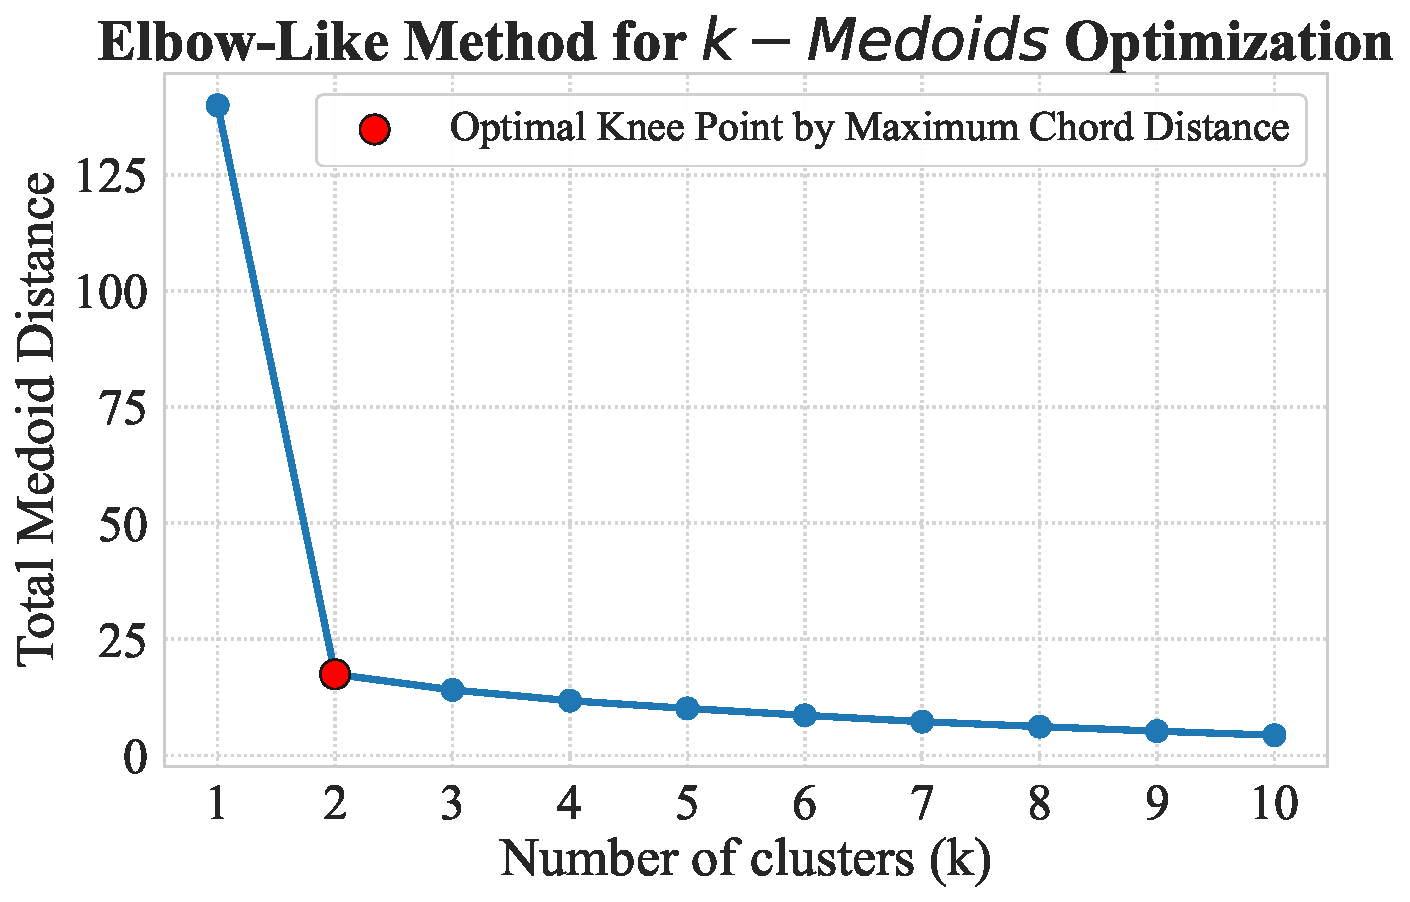
\includegraphics[width=0.95\linewidth]{./clustering/kmedoids/pdf/kmedoids_elbow_method.pdf}
    \caption{Διάγραμμα συνολικού κόστους του αλγορίθμου \textit{k-Medoids} για το \textit{Kundur Two-Area System}.}
    \label{fig:k_medoids_elbow_kundur}
\end{figure}

\begin{figure}[htbp]
    \centering
    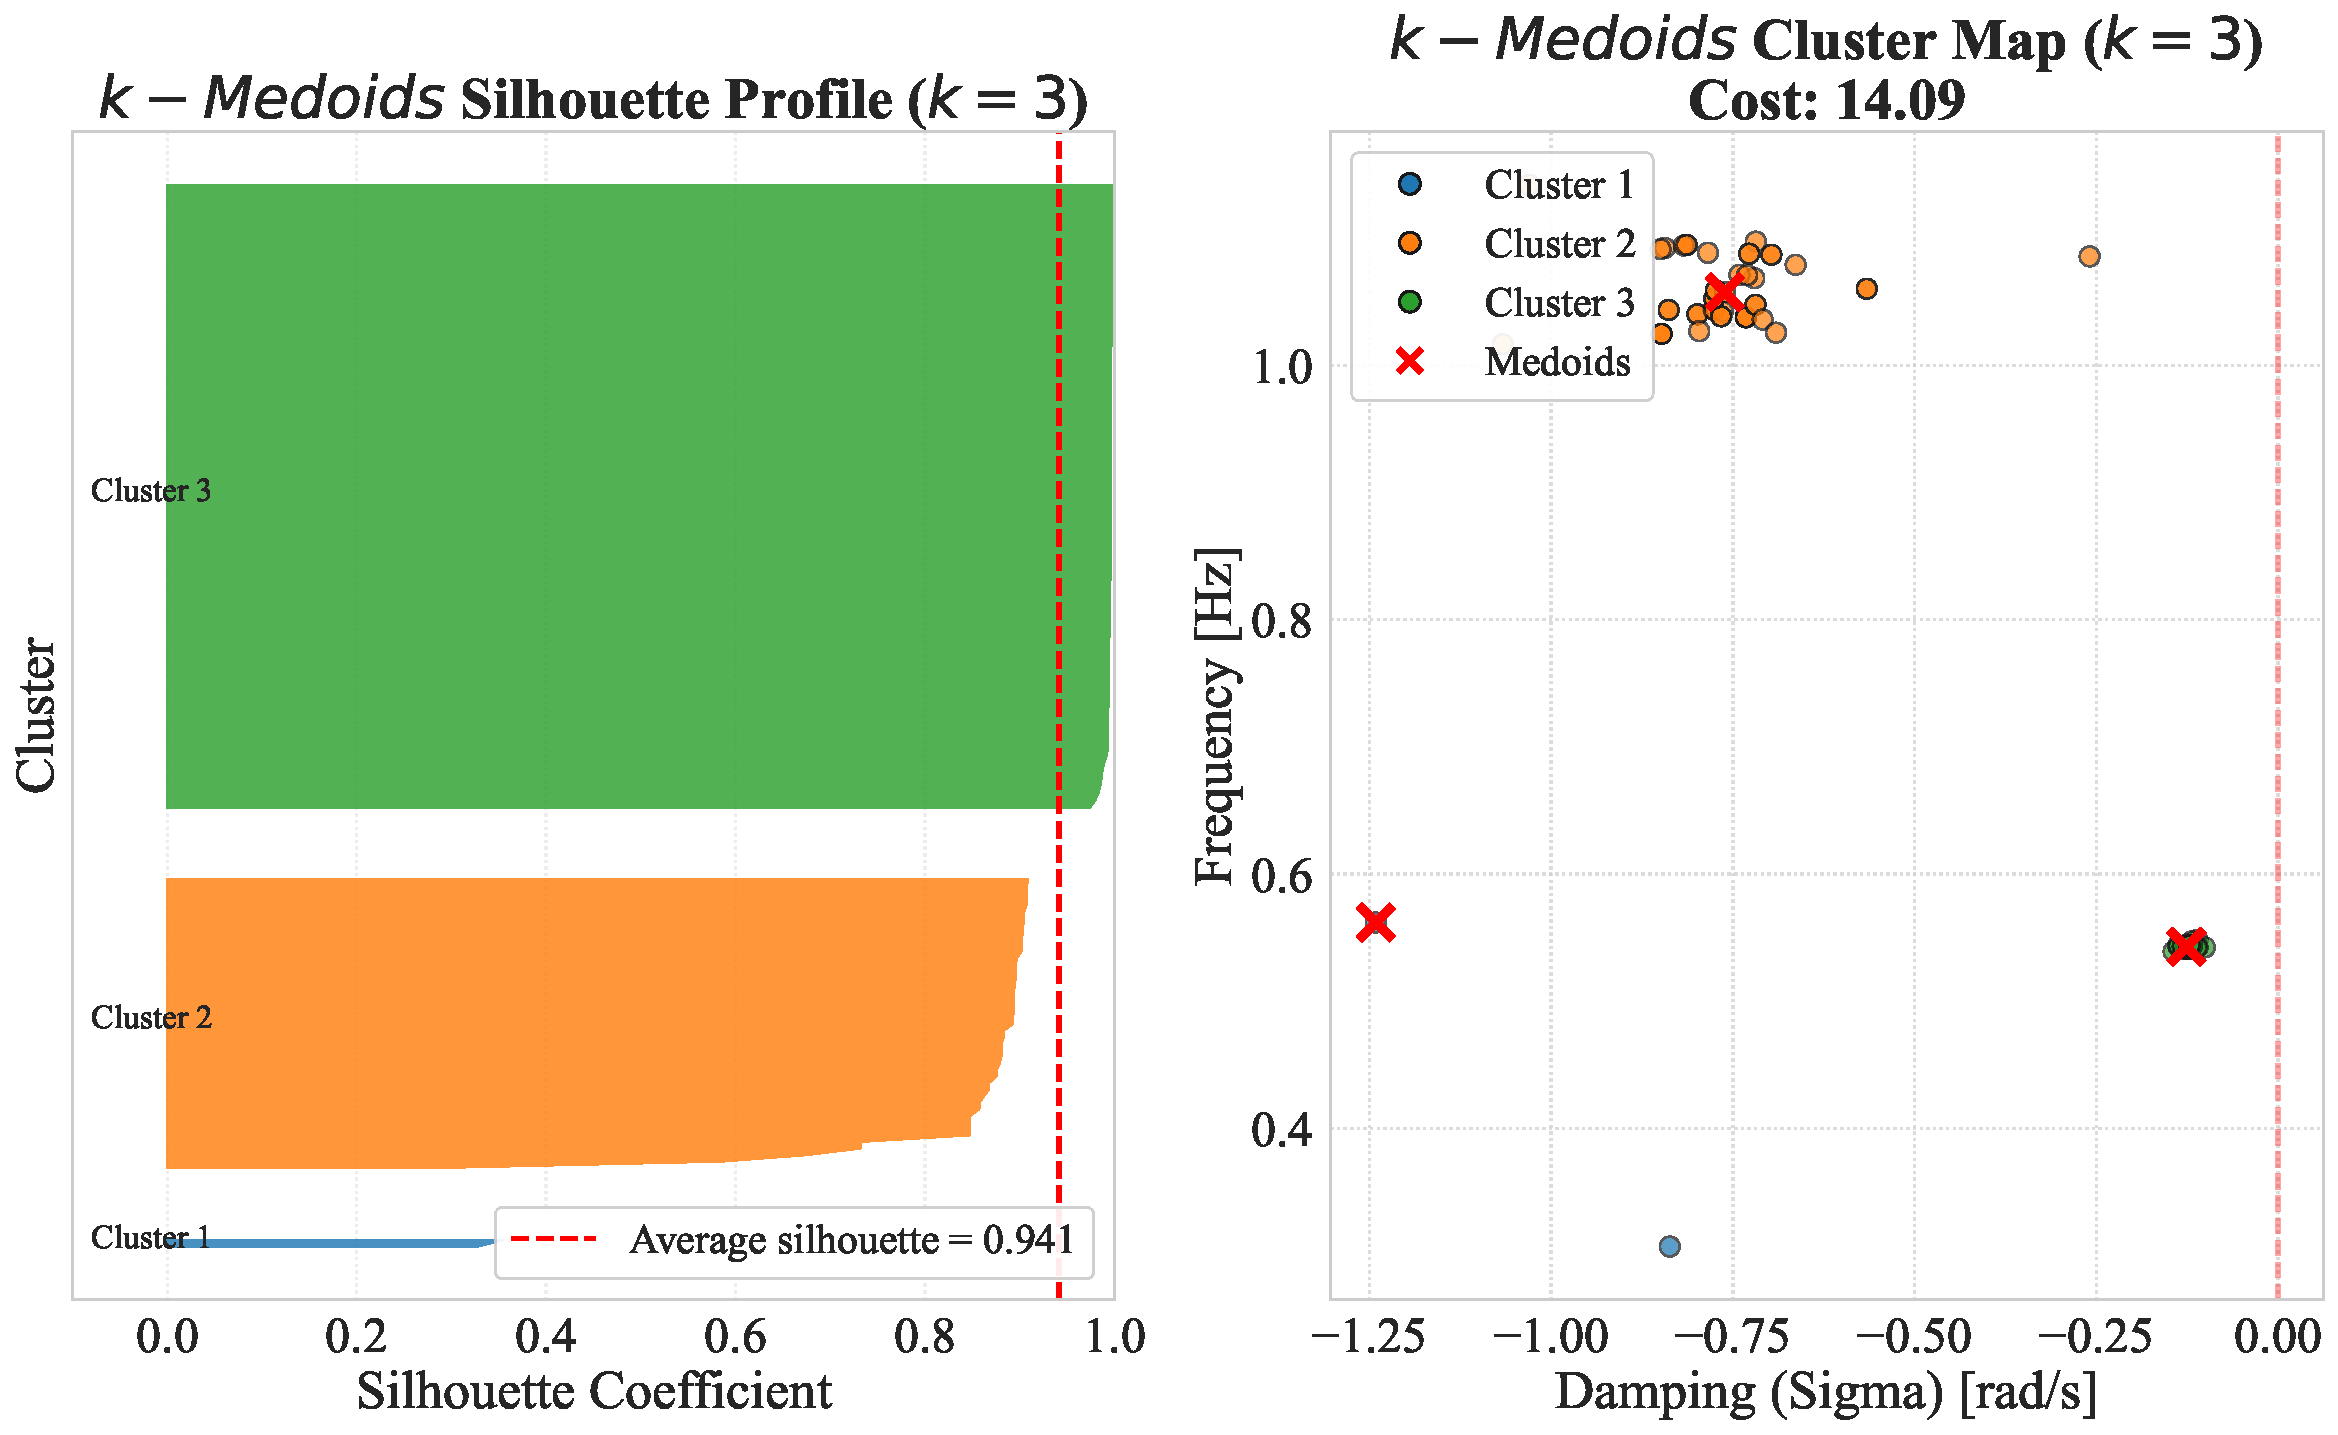
\includegraphics[width=0.95\linewidth]{./clustering/silhouette/pdf/silhouette_profile_kmedoids.pdf}
    \caption{Silhouette profile του αλγορίθμου \textit{k-Medoids} για $k=3$ στο \textit{Kundur Two-Area System}.}
    \label{fig:k_medoids_silhouette_kundur}
\end{figure}

\paragraph{Συγκριτική αξιολόγηση των αποτελεσμάτων}
Η εφαρμογή των δύο διαφορετικών αλγορίθμων ομαδοποίησης οδήγησε σε συγκλίνοντα συμπεράσματα, ενισχύοντας την αξιοπιστία της ανάλυσης. Ειδικότερα, τόσο ο \textit{k-Means} όσο και ο \textit{k-Medoids}, μέσω της τεχνικής \textit{Maximum Chord Distance}, υπέδειξαν ως βέλτιστο αριθμό συστάδων το $k=2$, ενώ η μέθοδος \textit{Silhouette} υπέδειξε και για τις δύο μεθόδους το $k=3$. Και στις δύο περιπτώσεις, όμως, η πρόσθετη τρίτη συστάδα αντιστοιχεί σε πολύ μικρό πλήθος ακραίων σημείων και δεν αναιρεί τον βασικό φυσικό διαχωρισμό μεταξύ της \textit{inter-area} περιοχής και της ευρύτερης \textit{intra-area} περιοχής, όπως αναφέρθηκε προηγουμένως.

Για την τελική επικύρωση της ταυτοποίησης, στο Table~\ref{tab:clustering_comparison_kundur} παρατίθεται η σύγκριση μεταξύ των συντεταγμένων των κέντρων που προέκυψαν από τη συσταδοποίηση και των θεωρητικών ιδιοτιμών αναφοράς του συστήματος, όπως αυτές δίνονται στον Πίνακα~\ref{tab:kundur_reference_modes}. 

\begin{table}[htbp]
\centering
\caption{\textsc{Σύγκριση κέντρων συσταδοποίησης με θεωρητικές ιδιοτιμές αναφοράς}}
\label{tab:clustering_comparison_kundur}
\footnotesize
\setlength{\tabcolsep}{3.5pt}
\renewcommand{\arraystretch}{1.12}
\begin{tabular}{lcccc}
\toprule
\textbf{Μέθοδος} & \multicolumn{2}{c}{\textbf{\textit{Inter-area}}} & \multicolumn{2}{c}{\textbf{\textit{Intra-area}}} \\
\cmidrule(lr){2-3}\cmidrule(lr){4-5}
& \textbf{$f$} & \textbf{$\sigma$} & \textbf{$f$} & \textbf{$\sigma$} \\
& \textbf{[Hz]} & \textbf{[rad/s]} & \textbf{[Hz]} & \textbf{[rad/s]} \\
\midrule
Θεωρ. αναφορά & 0.540 & -0.127 & 1.083 / 1.119 & -0.603 / -0.631 \\
\textit{k}-Means   & 0.540 & -0.133 & 1.049 & -0.770 \\
\textit{k}-Medoids & 0.543 & -0.126 & 1.057 & -0.761 \\
\bottomrule
\end{tabular}
\end{table}

\subsubsection{Αποτελέσματα για το \textit{IEEE 39-Bus}}
Στο σύστημα \textit{IEEE 39-Bus} η συσταδοποίηση έγινε ανά περιοχή ελέγχου. Γιά κάθε περιοχή ελέγχου, εφαρμόστηκε η ίδια μεθοδολογία που περιγράφηκε στην αρχή της ενότητας.
\paragraph{Αποτελέσματα k-Means}
Τα αποτελέσματα του αλγορίθμου \textit{k-Means} παρουσιάζονται χωριστά για κάθε περιοχή ελέγχου. Αρχικά, ο δείκτης WCSS ως συνάρτηση του αριθμού συστάδων παρουσιάζεται στα Figures~\ref{fig:k_means_elbow_ieee39_area1}--\ref{fig:k_means_elbow_ieee39_area3} και η εφαρμογή της τεχνικής \textit{Maximum Chord Distance} οδήγησε στην επιλογή των τιμών $k=4$ και για τις τρείς περιοχές ελέγχου. Στην συνέχεια, η ανάλυση με τη μέθοδο \textit{Silhouette} παρουσιάζεται στα Figures~\ref{fig:k_means_silhouette_ieee39_area1}--\ref{fig:k_means_silhouette_ieee39_area3} και δείχνει οτι η μέση τιμή του \textit{Silhouette Score} μεγιστοποιείται για διαφορετικές τιμές του $k$ σε κάθε περιοχή ελέγχου, συγκεκριμένα για $k=9$ στην περιοχή ελέγχου 1, $k=5$ στην περιοχή ελέγχου 2 και $k=7$ στην περιοχή ελέγχου 3. Αξίζει να σημειωθεί οτί τα \textit{Average Silhouette Scores} για τις τρείς περιοχές του \textit{IEEE 39-Bus} είναι μικρότερα απο τα αντίστοιχα του \textit{Kundur Two-Area}, ενώ ταυτόχρονα εμφανίζονται και ορισμένες αρνητικές τιμές \textit{Silhouette Score} για εκτίμωμενους ρυθμούς της συστάδας~2 της περιοχής ελέγχου~2, που υποδηλώνουν πιθανή αδυναμία διαχωρισμού του αλγορίθμου.

\begin{figure}[htbp]
    \centering
    \includegraphics[width=0.95\linewidth]{../IEEE39/analysis/Load03_Pplus2_50s_0.2_to_end_reset/clustering/by_control_area/area_1/kmeans/pdf/elbow_selected_kmeans.pdf}
    \caption{Διάγραμμα Elbow του αλγορίθμου \textit{k-Means} για την περιοχή ελέγχου 1 του \textit{IEEE 39-Bus System}.}
    \label{fig:k_means_elbow_ieee39_area1}
\end{figure}
\begin{figure}[htbp]
    \centering
    \includegraphics[width=0.95\linewidth]{../IEEE39/analysis/Load03_Pplus2_50s_0.2_to_end_reset/clustering/by_control_area/area_2/kmeans/pdf/elbow_selected_kmeans.pdf}
    \caption{Διάγραμμα Elbow του αλγορίθμου \textit{k-Means} για την περιοχή ελέγχου 2 του \textit{IEEE 39-Bus System}.}
    \label{fig:k_means_elbow_ieee39_area2}
\end{figure}
\begin{figure}[htbp]
    \centering
    \includegraphics[width=0.95\linewidth]{../IEEE39/analysis/Load03_Pplus2_50s_0.2_to_end_reset/clustering/by_control_area/area_3/kmeans/pdf/elbow_selected_kmeans.pdf}
    \caption{Διάγραμμα Elbow του αλγορίθμου \textit{k-Means} για την περιοχή ελέγχου 3 του \textit{IEEE 39-Bus System}.}
    \label{fig:k_means_elbow_ieee39_area3}
\end{figure}
\begin{figure}[htbp]
    \centering
    
\includegraphics[width=0.95\linewidth]{../IEEE39/analysis/Load03_Pplus2_50s_0.2_to_end_reset/clustering/by_control_area/area_1/silhouette/pdf/silhouette_profile_kmeans.pdf}
    \caption{Silhouette profile του αλγορίθμου \textit{k-Means} για $k=9$ στην περιοχή ελέγχου 1 του \textit{IEEE 39-Bus System}.}
    \label{fig:k_means_silhouette_ieee39_area1}
\end{figure}
\begin{figure}[htbp]
    \centering
    
\includegraphics[width=0.95\linewidth]{../IEEE39/analysis/Load03_Pplus2_50s_0.2_to_end_reset/clustering/by_control_area/area_2/silhouette/pdf/silhouette_profile_kmeans.pdf}
    \caption{Silhouette profile του αλγορίθμου \textit{k-Means} για $k=5$ στην περιοχή ελέγχου 2 του \textit{IEEE 39-Bus System}.}
    \label{fig:k_means_silhouette_ieee39_area2}
\end{figure}
\begin{figure}[htbp]
    \centering
    
\includegraphics[width=0.95\linewidth]{../IEEE39/analysis/Load03_Pplus2_50s_0.2_to_end_reset/clustering/by_control_area/area_3/silhouette/pdf/silhouette_profile_kmeans.pdf}
    \caption{Silhouette profile του αλγορίθμου \textit{k-Means} για $k=7$ στην περιοχή ελέγχου 3 του \textit{IEEE 39-Bus System}.}
    \label{fig:k_means_silhouette_ieee39_area3}
\end{figure}


\paragraph{Αποτελέσματα k-Medoids}
Όμοια με προηγουμένως, το συνολικό κόστος συσταδοποίησης του αλγορίθμου \textit{k-Medoids} ως συνάρτηση του αριθμού συστάδων παρουσιάζεται στα Figures~\ref{fig:k_medoids_elbow_ieee39_area1}--\ref{fig:k_medoids_elbow_ieee39_area3} και η εφαρμογή της τεχνικής \textit{Maximum Chord Distance} οδήγησε στην επιλογή της τιμής $k = 4$ και για τις τρείς περιοχές ελέγχου, σε πλήρη συμφωνία με τα αποτελέσματα του \textit{k-Means}. Η ανάλυση με τη μέθοδο \textit{Silhouette} παρουσιάζεται στα Figures~\ref{fig:k_medoids_silhouette_ieee39_area1}--\ref{fig:k_medoids_silhouette_ieee39_area3} και δείχνει ότι η μέση τιμή του \textit{Silhouette Score} μεγιστοποιείται για $k=8$ στην περιοχή ελέγχου 1, $k=4$ στην περιοχή ελέγχου 2 και $k=6$ στην περιοχή ελέγχου 3.
\begin{figure}[htbp]
    \centering
    \includegraphics[width=0.95\linewidth]{../IEEE39/analysis/Load03_Pplus2_50s_0.2_to_end_reset/clustering/by_control_area/area_1/kmedoids/pdf/elbow_selected_kmedoids.pdf}
    \caption{Διάγραμμα Elbow του αλγορίθμου \textit{k-Medoids} για την περιοχή ελέγχου 1 του \textit{IEEE 39-Bus System}.}
    \label{fig:k_medoids_elbow_ieee39_area1}
\end{figure}
\begin{figure}[htbp]
    \centering
    \includegraphics[width=0.95\linewidth]{../IEEE39/analysis/Load03_Pplus2_50s_0.2_to_end_reset/clustering/by_control_area/area_2/kmedoids/pdf/elbow_selected_kmedoids.pdf}
    \caption{Διάγραμμα Elbow του αλγορίθμου \textit{k-Medoids} για την περιοχή ελέγχου 2 του \textit{IEEE 39-Bus System}.}
    \label{fig:k_medoids_elbow_ieee39_area2}
\end{figure}
\begin{figure}[htbp]
    \centering
    \includegraphics[width=0.95\linewidth]{../IEEE39/analysis/Load03_Pplus2_50s_0.2_to_end_reset/clustering/by_control_area/area_3/kmedoids/pdf/elbow_selected_kmedoids.pdf}
    \caption{Διάγραμμα Elbow του αλγορίθμου \textit{k-Medoids} για την περιοχή ελέγχου 3 του \textit{IEEE 39-Bus System}.}
    \label{fig:k_medoids_elbow_ieee39_area3}
\end{figure}
\begin{figure}[htbp]
    \centering
    
\includegraphics[width=0.95\linewidth]{../IEEE39/analysis/Load03_Pplus2_50s_0.2_to_end_reset/clustering/by_control_area/area_1/silhouette/pdf/silhouette_profile_kmedoids.pdf}
    \caption{Silhouette profile του αλγορίθμου \textit{k-Medoids} για $k=8$ στην περιοχή ελέγχου 1 του \textit{IEEE 39-Bus System}.}
    \label{fig:k_medoids_silhouette_ieee39_area1}
\end{figure}
\begin{figure}[htbp]
    \centering
    
\includegraphics[width=0.95\linewidth]{../IEEE39/analysis/Load03_Pplus2_50s_0.2_to_end_reset/clustering/by_control_area/area_2/silhouette/pdf/silhouette_profile_kmedoids.pdf}
    \caption{Silhouette profile του αλγορίθμου \textit{k-Medoids} για $k=4$ στην περιοχή ελέγχου 2 του \textit{IEEE 39-Bus System}.}
    \label{fig:k_medoids_silhouette_ieee39_area2}
\end{figure}
\begin{figure}[htbp]
    \centering
    
\includegraphics[width=0.95\linewidth]{../IEEE39/analysis/Load03_Pplus2_50s_0.2_to_end_reset/clustering/by_control_area/area_3/silhouette/pdf/silhouette_profile_kmedoids.pdf}
    \caption{Silhouette profile του αλγορίθμου \textit{k-Medoids} για $k=6$ στην περιοχή ελέγχου 3 του \textit{IEEE 39-Bus System}.}
    \label{fig:k_medoids_silhouette_ieee39_area3}
\end{figure}

\paragraph{Συγκριτική Αξιολόγηση των αποτελεσμάτων}
Η εφαρμογή των δύο διαφορετικών αλγορίθμων συσταδοποίησης στο σύστημα \textit{IEEE 39-Bus} οδήγησε σε συγκλίνοντα αποτελέσματα όσο αφορά τον βέλτιστο αριθμό συστάδων χρησιμοποιώντας την \textit{Elbow} μέθοδο και τον  δείκτη WCSS. Στην ανάλυση όμως με τη μέθοδο \textit{Silhouette} προέκυψαν διαφορετικές βέλτιστες τιμές για τον αριθμό των συστάδων για τους δύο αλγόριθμους συσταδοποίησης. Ακόμα, μεγάλη απόκλιση μεταξύ τους, παρουσιάζουν και οι δύο τρόποι επιλογής του βέλτιστου αριθμού συστάδων.


\section{Συμπεράσματα}
Η παρούσα διερεύνηση έδειξε ότι η μέθοδος \textit{Matrix Pencil} μπορεί να χρησιμοποιηθεί αποτελεσματικά για την ταυτοποίηση ηλεκτρομηχανικών ταλαντώσεων από αποκρίσεις \textit{ringdown}. Η ποιότητα της μαθηματικής ανακατασκευής των σημάτων και η συνέπεια των εκτιμήσεων ως προς τα βιβλιογραφικά modes αναφοράς επιβεβαιώνουν ότι η συνολική μεθοδολογία είναι κατάλληλη για την ανάλυση της δυναμικής συμπεριφοράς των εξεταζόμενων συστημάτων.

Για το \textit{Kundur Two-Area System}, τα αποτελέσματα ήταν πιο καθαρά και πιο εύκολα στην ερμηνεία. Ο κυρίαρχος \textit{inter-area} mode εντοπίστηκε με συνέπεια κοντά στα $0.54$~Hz, ενώ οι \textit{intra-area} ταλαντώσεις εμφανίστηκαν στην περιοχή περίπου $1.0$--$1.1$~Hz. Παράλληλα, η ανακατασκευή των σημάτων παρουσίασε πολύ υψηλή πιστότητα, γεγονός που ενισχύει την αξιοπιστία των εξαγόμενων ιδιοτιμών.

Για το \textit{IEEE 39-Bus System}, η εικόνα ήταν πιο σύνθετη, όπως ήταν αναμενόμενο λόγω της μεγαλύτερης κλίμακας  του συστήματος. Παρότι οι εκτιμήσεις εμφανίζουν μεγαλύτερη διασπορά, η ανάλυση παραμένει συμβατή με τα modes αναφοράς της βιβλιογραφίας και επιτρέπει την ανάδειξη των βασικών περιοχών ταλαντωτικής συμπεριφοράς ανά περιοχή ελέγχου.

Τέλος, το στάδιο \textit{data screening} και η συμπληρωματική εφαρμογή τεχνικών συσταδοποίησης αποδείχθηκαν χρήσιμα για την οργάνωση και την ερμηνεία των αποτελεσμάτων. Συνολικά, η ροή εργασίας από το \textit{PowerFactory} στην \textit{Python} παρέχει μια συνεπή βάση για περαιτέρω αυτοματοποιημένη ανάλυση της δυναμικής ευστάθειας σε συστήματα ηλεκτρικής ενέργειας.

\FloatBarrier
\bibliographystyle{ieeetr}
\bibliography{../references}

\end{document}
